% Options for packages loaded elsewhere
\PassOptionsToPackage{unicode}{hyperref}
\PassOptionsToPackage{hyphens}{url}
%
\documentclass[
  11pt,
]{article}
\usepackage{lmodern}
\usepackage{amssymb,amsmath}
\usepackage{ifxetex,ifluatex}
\ifnum 0\ifxetex 1\fi\ifluatex 1\fi=0 % if pdftex
  \usepackage[T1]{fontenc}
  \usepackage[utf8]{inputenc}
  \usepackage{textcomp} % provide euro and other symbols
\else % if luatex or xetex
  \usepackage{unicode-math}
  \defaultfontfeatures{Scale=MatchLowercase}
  \defaultfontfeatures[\rmfamily]{Ligatures=TeX,Scale=1}
\fi
% Use upquote if available, for straight quotes in verbatim environments
\IfFileExists{upquote.sty}{\usepackage{upquote}}{}
\IfFileExists{microtype.sty}{% use microtype if available
  \usepackage[]{microtype}
  \UseMicrotypeSet[protrusion]{basicmath} % disable protrusion for tt fonts
}{}
\makeatletter
\@ifundefined{KOMAClassName}{% if non-KOMA class
  \IfFileExists{parskip.sty}{%
    \usepackage{parskip}
  }{% else
    \setlength{\parindent}{0pt}
    \setlength{\parskip}{6pt plus 2pt minus 1pt}}
}{% if KOMA class
  \KOMAoptions{parskip=half}}
\makeatother
\usepackage{xcolor}
\IfFileExists{xurl.sty}{\usepackage{xurl}}{} % add URL line breaks if available
\IfFileExists{bookmark.sty}{\usepackage{bookmark}}{\usepackage{hyperref}}
\hypersetup{
  pdftitle={Machine Learning Analysis applied to Investment strategies},
  pdfauthor={Antonio Malatesta; Karan Soneja; Michele D'Ambrosio},
  hidelinks,
  pdfcreator={LaTeX via pandoc}}
\urlstyle{same} % disable monospaced font for URLs
\usepackage[margin=1in]{geometry}
\usepackage{color}
\usepackage{fancyvrb}
\newcommand{\VerbBar}{|}
\newcommand{\VERB}{\Verb[commandchars=\\\{\}]}
\DefineVerbatimEnvironment{Highlighting}{Verbatim}{commandchars=\\\{\}}
% Add ',fontsize=\small' for more characters per line
\usepackage{framed}
\definecolor{shadecolor}{RGB}{248,248,248}
\newenvironment{Shaded}{\begin{snugshade}}{\end{snugshade}}
\newcommand{\AlertTok}[1]{\textcolor[rgb]{0.94,0.16,0.16}{#1}}
\newcommand{\AnnotationTok}[1]{\textcolor[rgb]{0.56,0.35,0.01}{\textbf{\textit{#1}}}}
\newcommand{\AttributeTok}[1]{\textcolor[rgb]{0.77,0.63,0.00}{#1}}
\newcommand{\BaseNTok}[1]{\textcolor[rgb]{0.00,0.00,0.81}{#1}}
\newcommand{\BuiltInTok}[1]{#1}
\newcommand{\CharTok}[1]{\textcolor[rgb]{0.31,0.60,0.02}{#1}}
\newcommand{\CommentTok}[1]{\textcolor[rgb]{0.56,0.35,0.01}{\textit{#1}}}
\newcommand{\CommentVarTok}[1]{\textcolor[rgb]{0.56,0.35,0.01}{\textbf{\textit{#1}}}}
\newcommand{\ConstantTok}[1]{\textcolor[rgb]{0.00,0.00,0.00}{#1}}
\newcommand{\ControlFlowTok}[1]{\textcolor[rgb]{0.13,0.29,0.53}{\textbf{#1}}}
\newcommand{\DataTypeTok}[1]{\textcolor[rgb]{0.13,0.29,0.53}{#1}}
\newcommand{\DecValTok}[1]{\textcolor[rgb]{0.00,0.00,0.81}{#1}}
\newcommand{\DocumentationTok}[1]{\textcolor[rgb]{0.56,0.35,0.01}{\textbf{\textit{#1}}}}
\newcommand{\ErrorTok}[1]{\textcolor[rgb]{0.64,0.00,0.00}{\textbf{#1}}}
\newcommand{\ExtensionTok}[1]{#1}
\newcommand{\FloatTok}[1]{\textcolor[rgb]{0.00,0.00,0.81}{#1}}
\newcommand{\FunctionTok}[1]{\textcolor[rgb]{0.00,0.00,0.00}{#1}}
\newcommand{\ImportTok}[1]{#1}
\newcommand{\InformationTok}[1]{\textcolor[rgb]{0.56,0.35,0.01}{\textbf{\textit{#1}}}}
\newcommand{\KeywordTok}[1]{\textcolor[rgb]{0.13,0.29,0.53}{\textbf{#1}}}
\newcommand{\NormalTok}[1]{#1}
\newcommand{\OperatorTok}[1]{\textcolor[rgb]{0.81,0.36,0.00}{\textbf{#1}}}
\newcommand{\OtherTok}[1]{\textcolor[rgb]{0.56,0.35,0.01}{#1}}
\newcommand{\PreprocessorTok}[1]{\textcolor[rgb]{0.56,0.35,0.01}{\textit{#1}}}
\newcommand{\RegionMarkerTok}[1]{#1}
\newcommand{\SpecialCharTok}[1]{\textcolor[rgb]{0.00,0.00,0.00}{#1}}
\newcommand{\SpecialStringTok}[1]{\textcolor[rgb]{0.31,0.60,0.02}{#1}}
\newcommand{\StringTok}[1]{\textcolor[rgb]{0.31,0.60,0.02}{#1}}
\newcommand{\VariableTok}[1]{\textcolor[rgb]{0.00,0.00,0.00}{#1}}
\newcommand{\VerbatimStringTok}[1]{\textcolor[rgb]{0.31,0.60,0.02}{#1}}
\newcommand{\WarningTok}[1]{\textcolor[rgb]{0.56,0.35,0.01}{\textbf{\textit{#1}}}}
\usepackage{longtable,booktabs}
% Correct order of tables after \paragraph or \subparagraph
\usepackage{etoolbox}
\makeatletter
\patchcmd\longtable{\par}{\if@noskipsec\mbox{}\fi\par}{}{}
\makeatother
% Allow footnotes in longtable head/foot
\IfFileExists{footnotehyper.sty}{\usepackage{footnotehyper}}{\usepackage{footnote}}
\makesavenoteenv{longtable}
\usepackage{graphicx,grffile}
\makeatletter
\def\maxwidth{\ifdim\Gin@nat@width>\linewidth\linewidth\else\Gin@nat@width\fi}
\def\maxheight{\ifdim\Gin@nat@height>\textheight\textheight\else\Gin@nat@height\fi}
\makeatother
% Scale images if necessary, so that they will not overflow the page
% margins by default, and it is still possible to overwrite the defaults
% using explicit options in \includegraphics[width, height, ...]{}
\setkeys{Gin}{width=\maxwidth,height=\maxheight,keepaspectratio}
% Set default figure placement to htbp
\makeatletter
\def\fps@figure{htbp}
\makeatother
\setlength{\emergencystretch}{3em} % prevent overfull lines
\providecommand{\tightlist}{%
  \setlength{\itemsep}{0pt}\setlength{\parskip}{0pt}}
\setcounter{secnumdepth}{5}
\usepackage{float}
\let\origfigure\figure
\let\endorigfigure\endfigure
\renewenvironment{figure}[1][2] {
    \expandafter\origfigure\expandafter[H]
} {
    \endorigfigure
}
\usepackage{booktabs}
\usepackage{longtable}
\usepackage{array}
\usepackage{multirow}
\usepackage{wrapfig}
\usepackage{float}
\usepackage{colortbl}
\usepackage{pdflscape}
\usepackage{tabu}
\usepackage{threeparttable}
\usepackage{threeparttablex}
\usepackage[normalem]{ulem}
\usepackage{makecell}
\usepackage{xcolor}
\usepackage[]{natbib}
\bibliographystyle{plainnat}

\title{Machine Learning Analysis applied to Investment strategies}
\usepackage{etoolbox}
\makeatletter
\providecommand{\subtitle}[1]{% add subtitle to \maketitle
  \apptocmd{\@title}{\par {\large #1 \par}}{}{}
}
\makeatother
\subtitle{Université Paris 1 Panthéon-Sorbonne

M2 IRFA Engineering of Financial Mathematics

X5I22919 Data Science Software

Module leader: Prof.~Bertrand K. Hassani}
\author{Antonio Malatesta\footnote{E-mail:\href{mailto:antonio.malatesta@outlook.com}{\nolinkurl{antonio.malatesta@outlook.com}}} \and Karan Soneja\footnote{E-mail:\href{mailto:sonejakaran@gmail.com}{\nolinkurl{sonejakaran@gmail.com}}} \and Michele D'Ambrosio\footnote{E-mail:\href{mailto:mi.dambrosio105@gmail.com}{\nolinkurl{mi.dambrosio105@gmail.com}}}}
\date{}

\begin{document}
\maketitle

{
\setcounter{tocdepth}{2}
\tableofcontents
}
\newpage

\hypertarget{introduction}{%
\section{Introduction}\label{introduction}}

The present report shows an implementation in R \footnote{\url{https://cran.r-project.org/}}
of three different Machine learning approaches to exploit historical
stock price data for making predictions on the stocks' future price
levels. We aim at understanding whether it is possible to obtain
profitable trading indications leading to a higher return than a passive
strategy. The remaining of the report is structured as follows. In
Section 3, trading operations are performed based on technical analysis
indicators. In section 4, we use instead neural network analysis to
develop an investment strategy, while in Section 5 a Random forest
algorithm is implemented.

\hypertarget{data}{%
\section{Data}\label{data}}

The data used in this report consists of the stock price of some of the
10 biggest publicly quoted French companies, as of September 2019
\footnote{The full list here:
  \url{https://live.euronext.com/en/product/indices/FR0003500008-XPAR/market-information}}.

\begin{table}[ht]
\caption{Top ten firms in CAC40 by market cap, September 2019}
\centering
\begin{tabular}{|c|c|c|c|}
  \hline
Company & MNEMO  &  Sector  & Weight\% \\
  \hline
  TOTAL &   FP  & Oil and Gas & 9,54 \\
  LVMH &    MC  & Personal and Household Goods & 7,97 \\
  SANOFI & SAN  & Health Care & 7,54 \\
  AIRBUS & AIR  & Industrial Goods and Services &   5,47 \\
  L'OREAL   & OR  & Personal and Household Goods &  5,10 \\
  AIR LIQUIDE & AI  & Chemicals &   4,40 \\
  DANONE &  BN  & Food and Beverage & 4,14 \\
  VINCI &   DG & Construction and Materials & 3,97 \\
  BNP PARIBAS ACT.A &   BNP  & Banks & 3,95 \\
  SAFRAN & SAF  & Industrial Goods and Services & 3,72 \\
   \hline
  \end{tabular}
\end{table}

With the following command, we can download the daily open, high, low,
close and adjusted prices, as well as the volume, of the stocks we
consider in our analysis, from 28/12/2012 to 31/12/2018.

\begin{Shaded}
\begin{Highlighting}[]
\NormalTok{quantmod}\OperatorTok{::}\KeywordTok{getSymbols}\NormalTok{(}\StringTok{"COMPANY CODE"}\NormalTok{, }\DataTypeTok{src=}\StringTok{"yahoo"}\NormalTok{, }
                     \DataTypeTok{from=}\StringTok{"2012-12-28"}\NormalTok{, }\DataTypeTok{to=}\StringTok{"2018-12-31"}\NormalTok{)}
\end{Highlighting}
\end{Shaded}

In some sections, we add economic and financial variables to test
whether they can increase the predictive power of the analysis. The
following table offers a detailed list of the variables considered.

\begin{table}[H]

\caption{\label{tab:first_half}Additional economical variables}
\centering
\begin{tabular}[t]{ll}
\toprule
Economic
Factors & Source\\
\midrule
Daily interest rate & sdw.ecb.europa.eu\\
Daily Exchange rate
(EUR/USD) & exchangerates.org\\
Political Stability (yearly) & databank.worldbank.org\\
CPI Infaltion (monthly) & www.inflation.eu\\
\bottomrule
\end{tabular}
\end{table}

Our hypothesis is that factors like inflation and interest rate might
have a big impact on companies' stock prices on a day-by-day basis. On
the other hand, we consider financial statement data that change only on
a yearly basis, checking whether black-box models can find connections
between the prices and the variables over a long-term horizon.

\begin{table}[H]

\caption{\label{tab:second_half}Additional financial statement variables}
\centering
\begin{tabular}[t]{ll}
\toprule
Yearly Financial
Statements Variables & Source\\
\midrule
Dividend & \\
Revenue & \\
Net income & dividenmax.com\\
Basic earnings
per share & \\
Diluted earnings
per share & airbus.com\\
\addlinespace
Total assets & \\
Intangible assets & airliquide.com\\
PPE & \\
Cash & danone.com\\
Total equity & \\
\addlinespace
Non current liability & vinci.com\\
Cash flows from operating activities & \\
Net cash flows from
investing activities & invest.bnpparibas.com\\
Net cash flows from
financing activities & \\
Net cash and cash
equivalents at end of period & \\
\bottomrule
\end{tabular}
\end{table}

As a last disclaimer, the code shown in the report has only an
explanatory purpose. We further attach the complete code to reproduce
the analysis.

\newpage

\hypertarget{technical-analysis-implementation-of-a-naive-strategy-in-r}{%
\section{Technical analysis: implementation of a naive strategy in
R}\label{technical-analysis-implementation-of-a-naive-strategy-in-r}}

As \citet{Brock1992} explain, \emph{technical analysis} (TA) is an
``attempt to forecast prices by the study of past prices and a few other
related summary statistics about security trading'' (pag 2). This
practice however clashes with the Efficient Market Hypotesis lied out by
\citet{Fama1970} , according to which market prices incorporate all
available information on the securities at any times.

Despite Fama's paper, which soon got traction among academia, the work
by \citet{Taylor1992} reports that practioners in the world largest
financial centres declare making use of Technical analysis, especially
for intraday and short-term period trading. This revamped a large stream
of research on the topic, to the point where complex optimization
algorithms (namely, of the class of evolutionary algorithms) were
introduced to get better predictions in terms of global optima search.
For example, genetic programming is implemented to avoid the human bias
in creating trading rules, letting the algorithms evaluate a series of
rules implemented at each search stage, picking the best features and
discarding the least performing ones. For a lengthier treatment on the
topic, the reader can refer to \citet{Neely1997}, or the more recent
\citet{Mousavi2014} .

\citet{Neftci1991} gives a proper formal charaterization of the main
classes of technical analysis indicators. He claims that ``any
well-defined technical analysis rule has to pass the test of being a
Markov time'', otherwise ``the procedure would be using future
information in order to issue such signals'' (pag. 8). Hence, relying
heavily on chart analysis can be misleading. A class of signals that
appear to be stopping times are those generated by moving average
indicators, which are those we use in the present section.

One caveat one should always keep in mind when talking about technical
analysis is that its predictive power can be biased upward by its
intrinsic self-fulfilling feature: if agents believe that TA can have
some predictive power, then following the trends will indeed let the
predicted events happen, as all agents will implement similar decisions,
given that they base their analysis on similar indicators.

\hypertarget{technical-analysis-indicators}{%
\subsection{Technical analysis
indicators}\label{technical-analysis-indicators}}

We will offer both a formal definition and a visual representation of
each TA indicator used. In the following charts, prices are represented
by the so-called `candlesticks'. The rectangular area will show the day
open and close, whereas the wicks represent the day high and low. The
green filling indicates that the security closed at a higher price than
the opening, whereas orange indicates a negative performance on a
day-basis. Trading volumes are also shown in the bottom part of the
first chart.

The first indicator is the \emph{simple moving average}. It is defined
as \begin{equation} 
SMA = \displaystyle \sum_{t=1}^{n} \frac{x_t}{n} 
\end{equation}

where \(x_t =\) the t-th price observation, for \(t \in \{1,...,n\}\).

\begin{Shaded}
\begin{Highlighting}[]
\KeywordTok{chartSeries}\NormalTok{(AIR.PA,}\CommentTok{# need '.PA' suffix for Paris CAC40}
            \DataTypeTok{type=}\StringTok{"matchsticks"}\NormalTok{,}
            \DataTypeTok{name =} \StringTok{"HLOC Candle chart and SMA, Air France"}\NormalTok{,}
            \DataTypeTok{theme=}\KeywordTok{chartTheme}\NormalTok{(}\StringTok{'white'}\NormalTok{)) }\CommentTok{# chart setting}

\NormalTok{quantmod}\OperatorTok{::}\KeywordTok{addSMA}\NormalTok{(}\DataTypeTok{n=}\DecValTok{50}\NormalTok{,}\DataTypeTok{on=}\DecValTok{1}\NormalTok{,}\DataTypeTok{col =} \StringTok{'blue'}\NormalTok{) }\CommentTok{# to overimpose SMA(50), in blue}
\NormalTok{quantmod}\OperatorTok{::}\KeywordTok{addSMA}\NormalTok{(}\DataTypeTok{n=}\DecValTok{200}\NormalTok{,}\DataTypeTok{on=}\DecValTok{1}\NormalTok{,}\DataTypeTok{col =} \StringTok{'purple'}\NormalTok{) }\CommentTok{# TA functions from 'TTR' }
\end{Highlighting}
\end{Shaded}

\begin{figure}
\centering
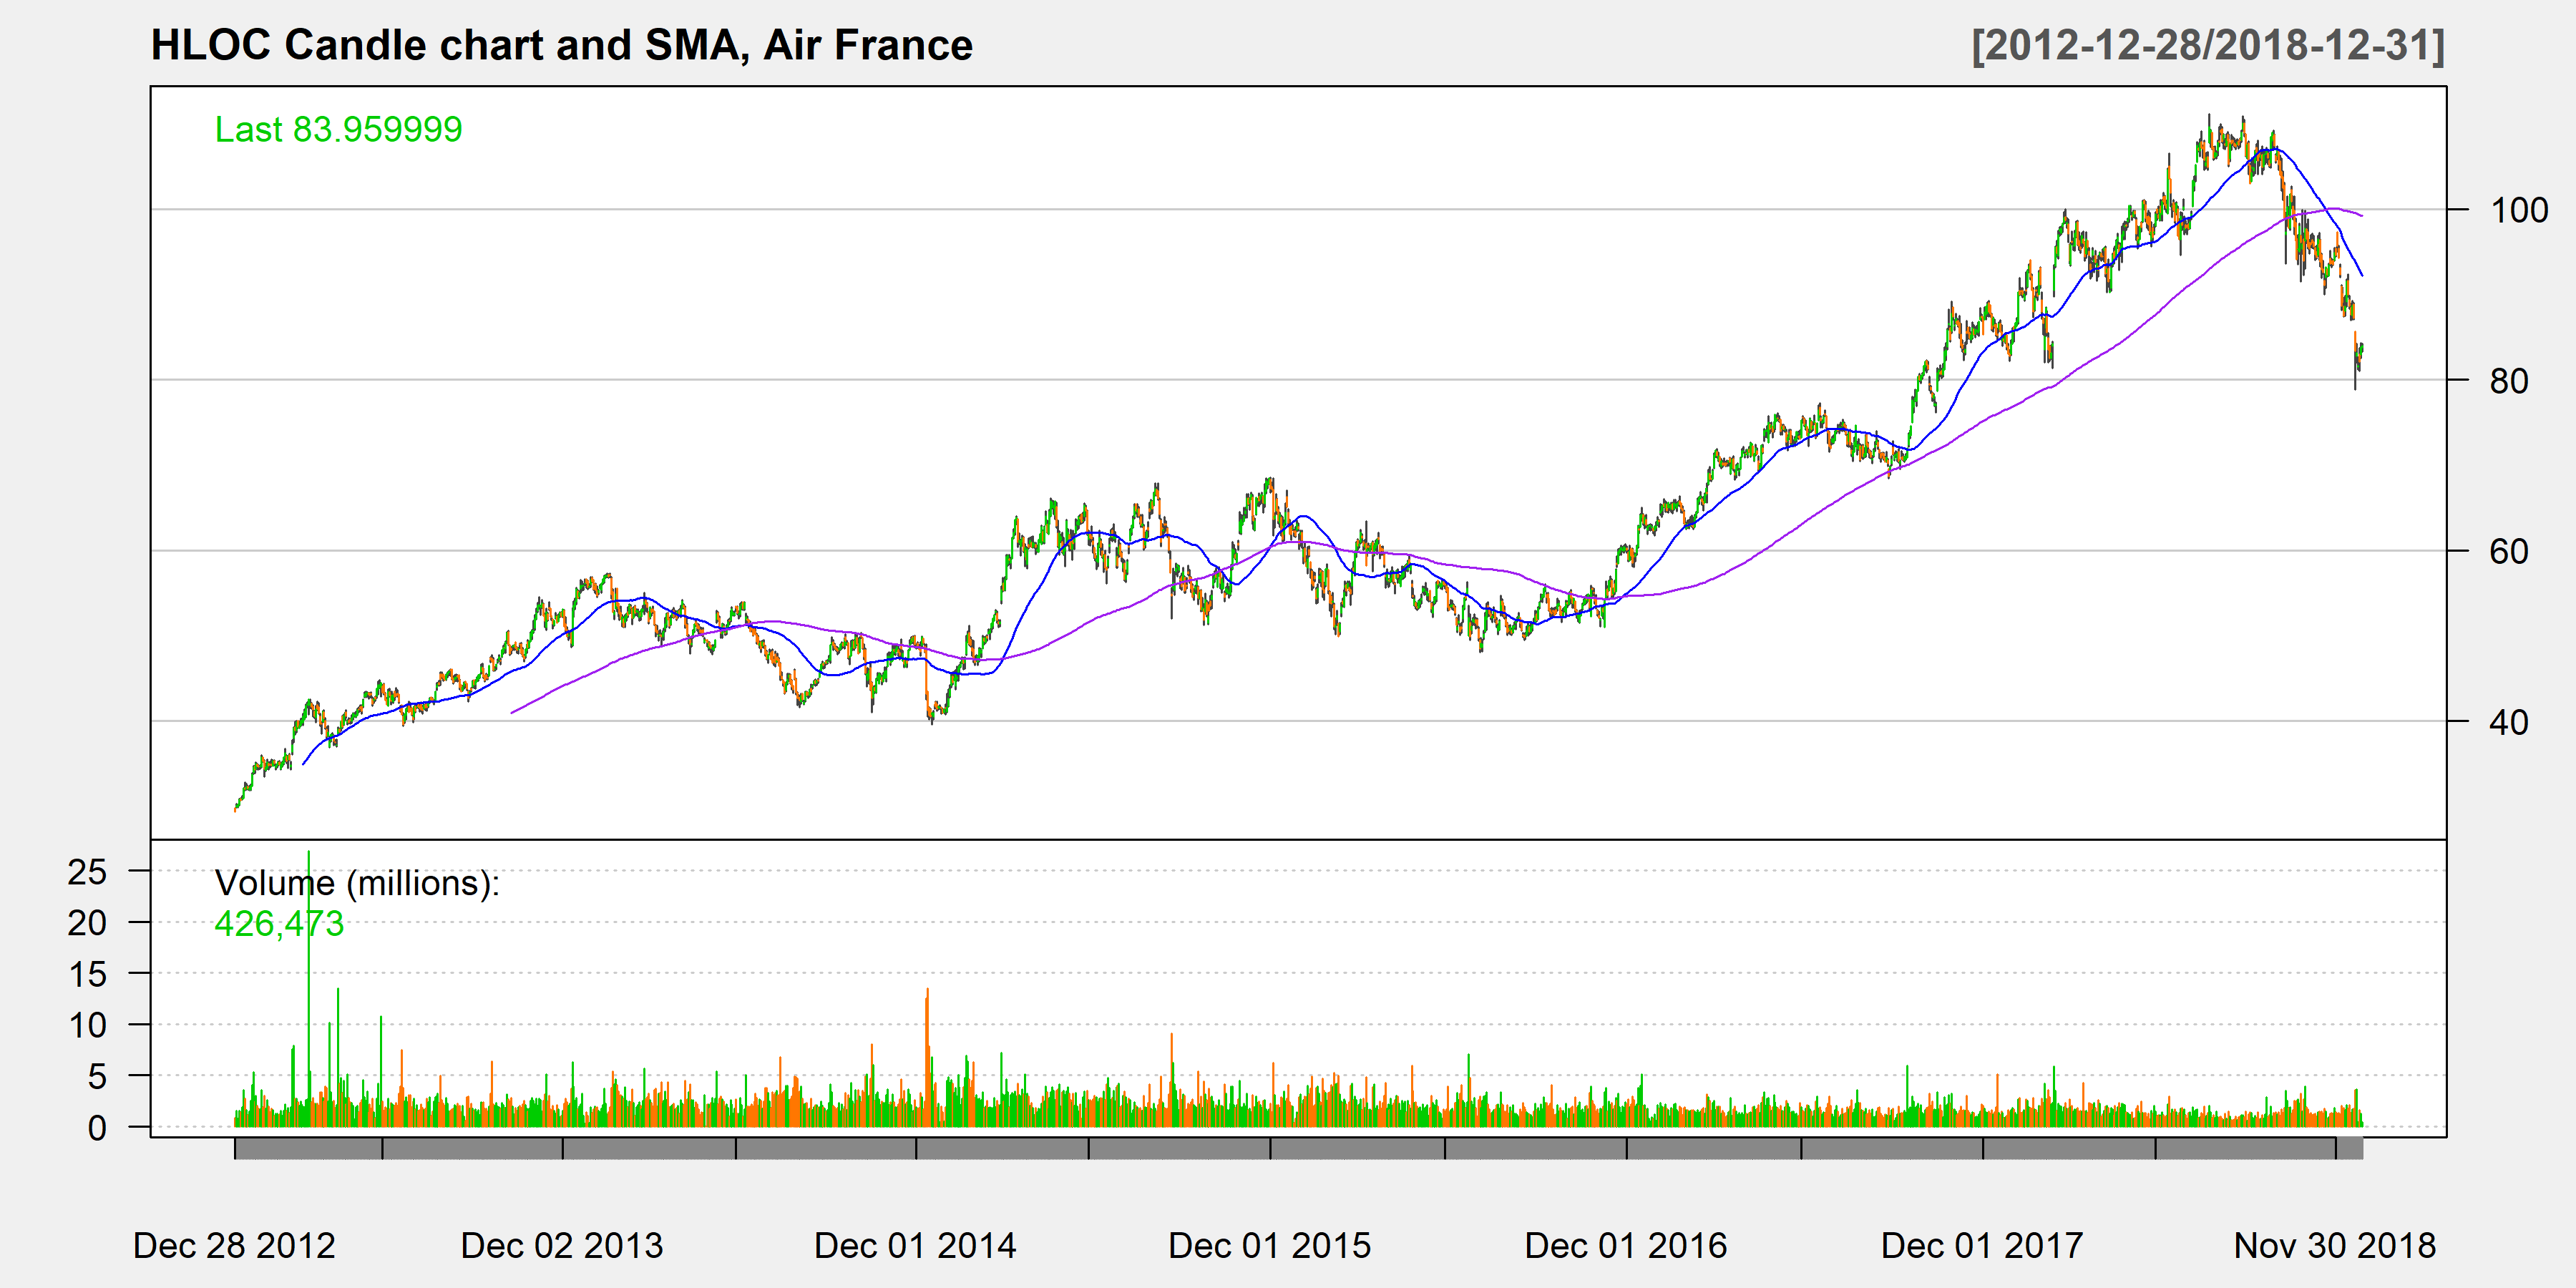
\includegraphics{"D:/2017-2018/data_analysis/technical_analysis/report/HLOC Candle chart and SMA, Air France.png"}
\caption{Daily HLOC Chart price, with SMA(50) in blu, and SMA(200) in
purple.}
\end{figure}

The SMA is used to smooth out the price trends from the short-term
fluctations. Usually, (at least) two SMA's of different time-lags are
used together to generate trading signals. The short-term average
crossing from below the long-term average is considered a buy signal,
whereas a crossing in the other direction is taken as an indication to
sell. One common choice for the lags are the 50- and the 200-days
averages. One could also consider shorter time windows, to retain the
short-term fluctations in the SMAs.

The second indicator is the \textbf{Relative Strength Index}, or RSI .
It is computed as\\
\begin{equation} 
RSI = 100 - \left( \frac{100}{(1 + \frac{\Delta_u}{\Delta_d} } \right) 
\end{equation} where \(\Delta_u =\) Average of Upward Price Change, and
\(\Delta_d =\) Average of Downward Price Change \footnote{\url{https://www.fidelity.com/learning-center/trading-investing/technical-analysis/technical-indicator-guide/RSI}}.
(See also \citet{Hsu2016} for an example of different parametrizations.)

The RSI is an oscillator, since its value is in the range {[}0,100{]}.
It gives indications on the \textbf{momentum}, that is, the ``the
magnitude of recent price changes to evaluate overbought or oversold
conditions in the price of a stock or other asset. \footnote{\url{https://www.investopedia.com/terms/r/rsi.asp}}''
Generally, \(RSI>70\) is taken as an indication for a security to be
overbought, whereas \(RSI < 30\) has the opposite meaning.

\begin{Shaded}
\begin{Highlighting}[]
\NormalTok{quantmod}\OperatorTok{::}\KeywordTok{addRSI}\NormalTok{(}\DataTypeTok{n=}\DecValTok{14}\NormalTok{, }\DataTypeTok{maType=} \StringTok{'SMA'}\NormalTok{) }
\CommentTok{# the RSI is shown, albeit not overimposed to the price pattern}
\end{Highlighting}
\end{Shaded}

\begin{figure}
\centering
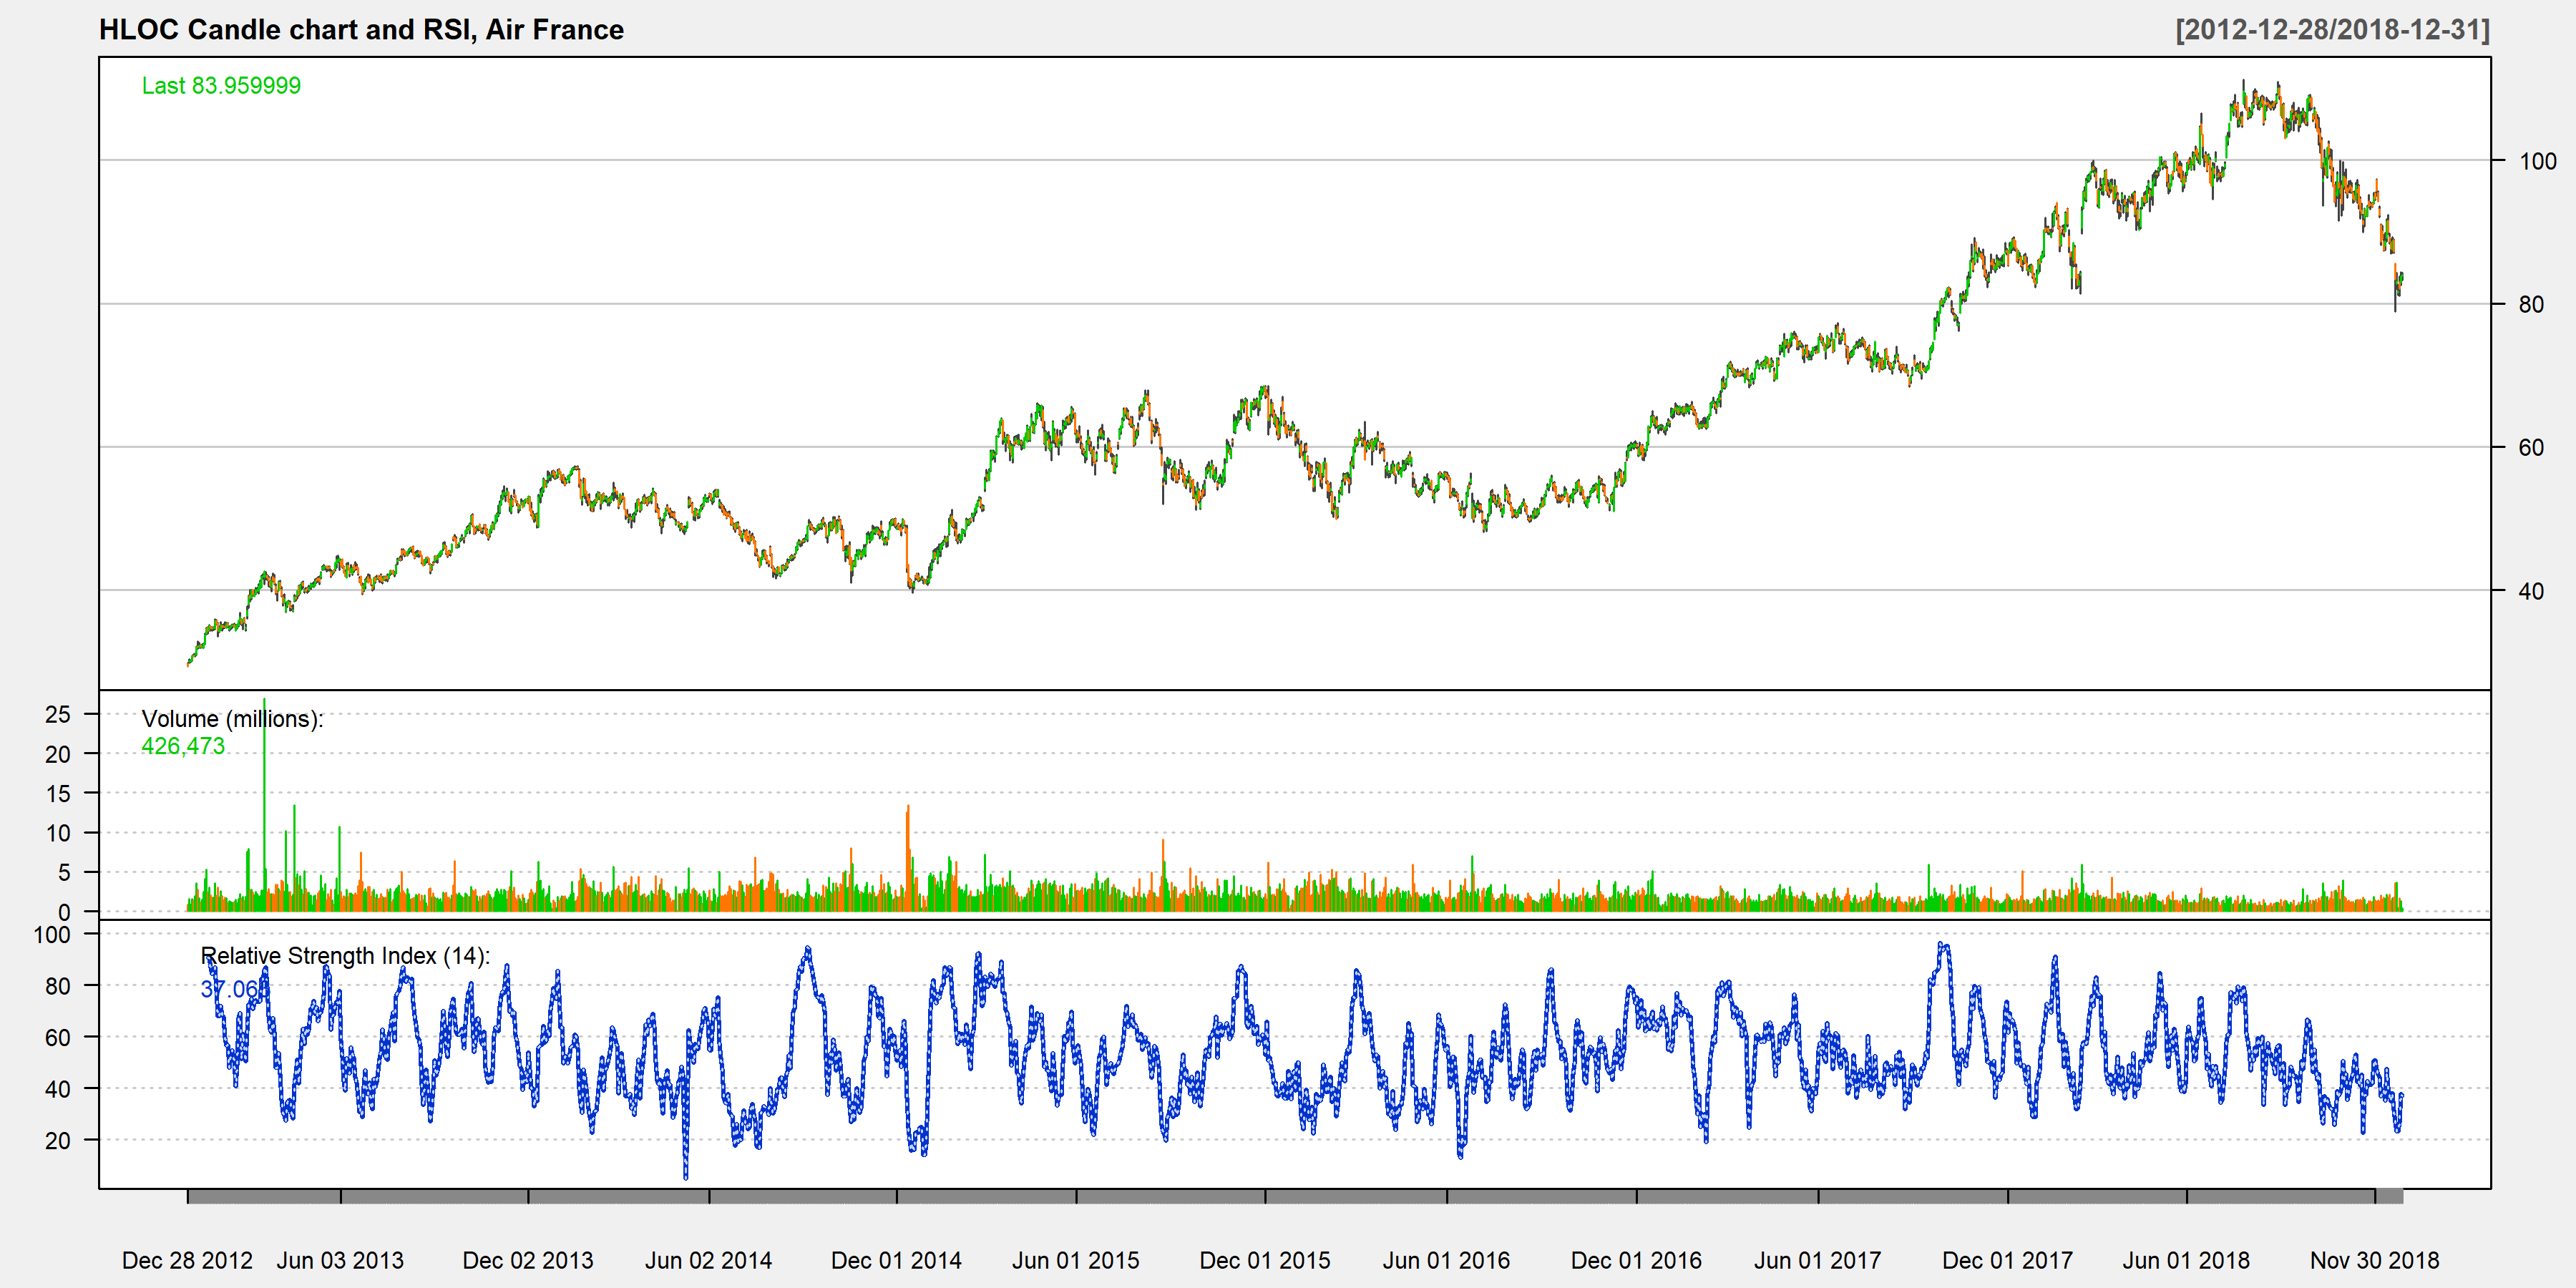
\includegraphics{"D:/2017-2018/data_analysis/technical_analysis/report/HLOC Candle chart and RSI, Air France.png"}
\caption{Daily HLOC Chart price with RSI(14)}
\end{figure}

The third indicator are the \textbf{Bollinger Bands} \footnote{\url{https://www.bollingerbands.com/}}.
These are defined by the plot of a simple moving average, as defined
below by the \(\mu\), along with its standard deviation around it,
defining the upper and lower bands. These are defined respectively as
\begin{equation}
B_u = MA(\mu, n) + m \cdot \sigma(\mu,n)
\end{equation} and \begin{equation}
B_d = MA(\mu, n) - m \cdot \sigma(\mu,n)
\end{equation}

with

\(HLC_t:=High_t +Low_t + Close_t\);

\(\mu= \frac{HLC_t}{3}\);

\(\sigma_n= \sqrt{\displaystyle \frac{\sum_{t=1}^{n} {(HLC_t-\mu)^2}}{n}}\)
the standard deviation of HLC over n days;

\(n \in \mathbb{N^*}\) the number of days over which the SMA is
computed;

\(m \in \mathbb{N^*}\) the number of standard deviations used to create
the width of the bands.

A common parametrization of this indicator is one with
two-standard-deviation-wide bands around a 20-day simple moving average
(i.e.~\(m=2\),\(n=20\)).

\begin{Shaded}
\begin{Highlighting}[]
\KeywordTok{addBBands}\NormalTok{(}\DataTypeTok{n=}\DecValTok{20}\NormalTok{, }\DataTypeTok{sd=}\DecValTok{2}\NormalTok{, }\DataTypeTok{maType=} \StringTok{"SMA"}\NormalTok{) }
\end{Highlighting}
\end{Shaded}

\begin{figure}
\centering
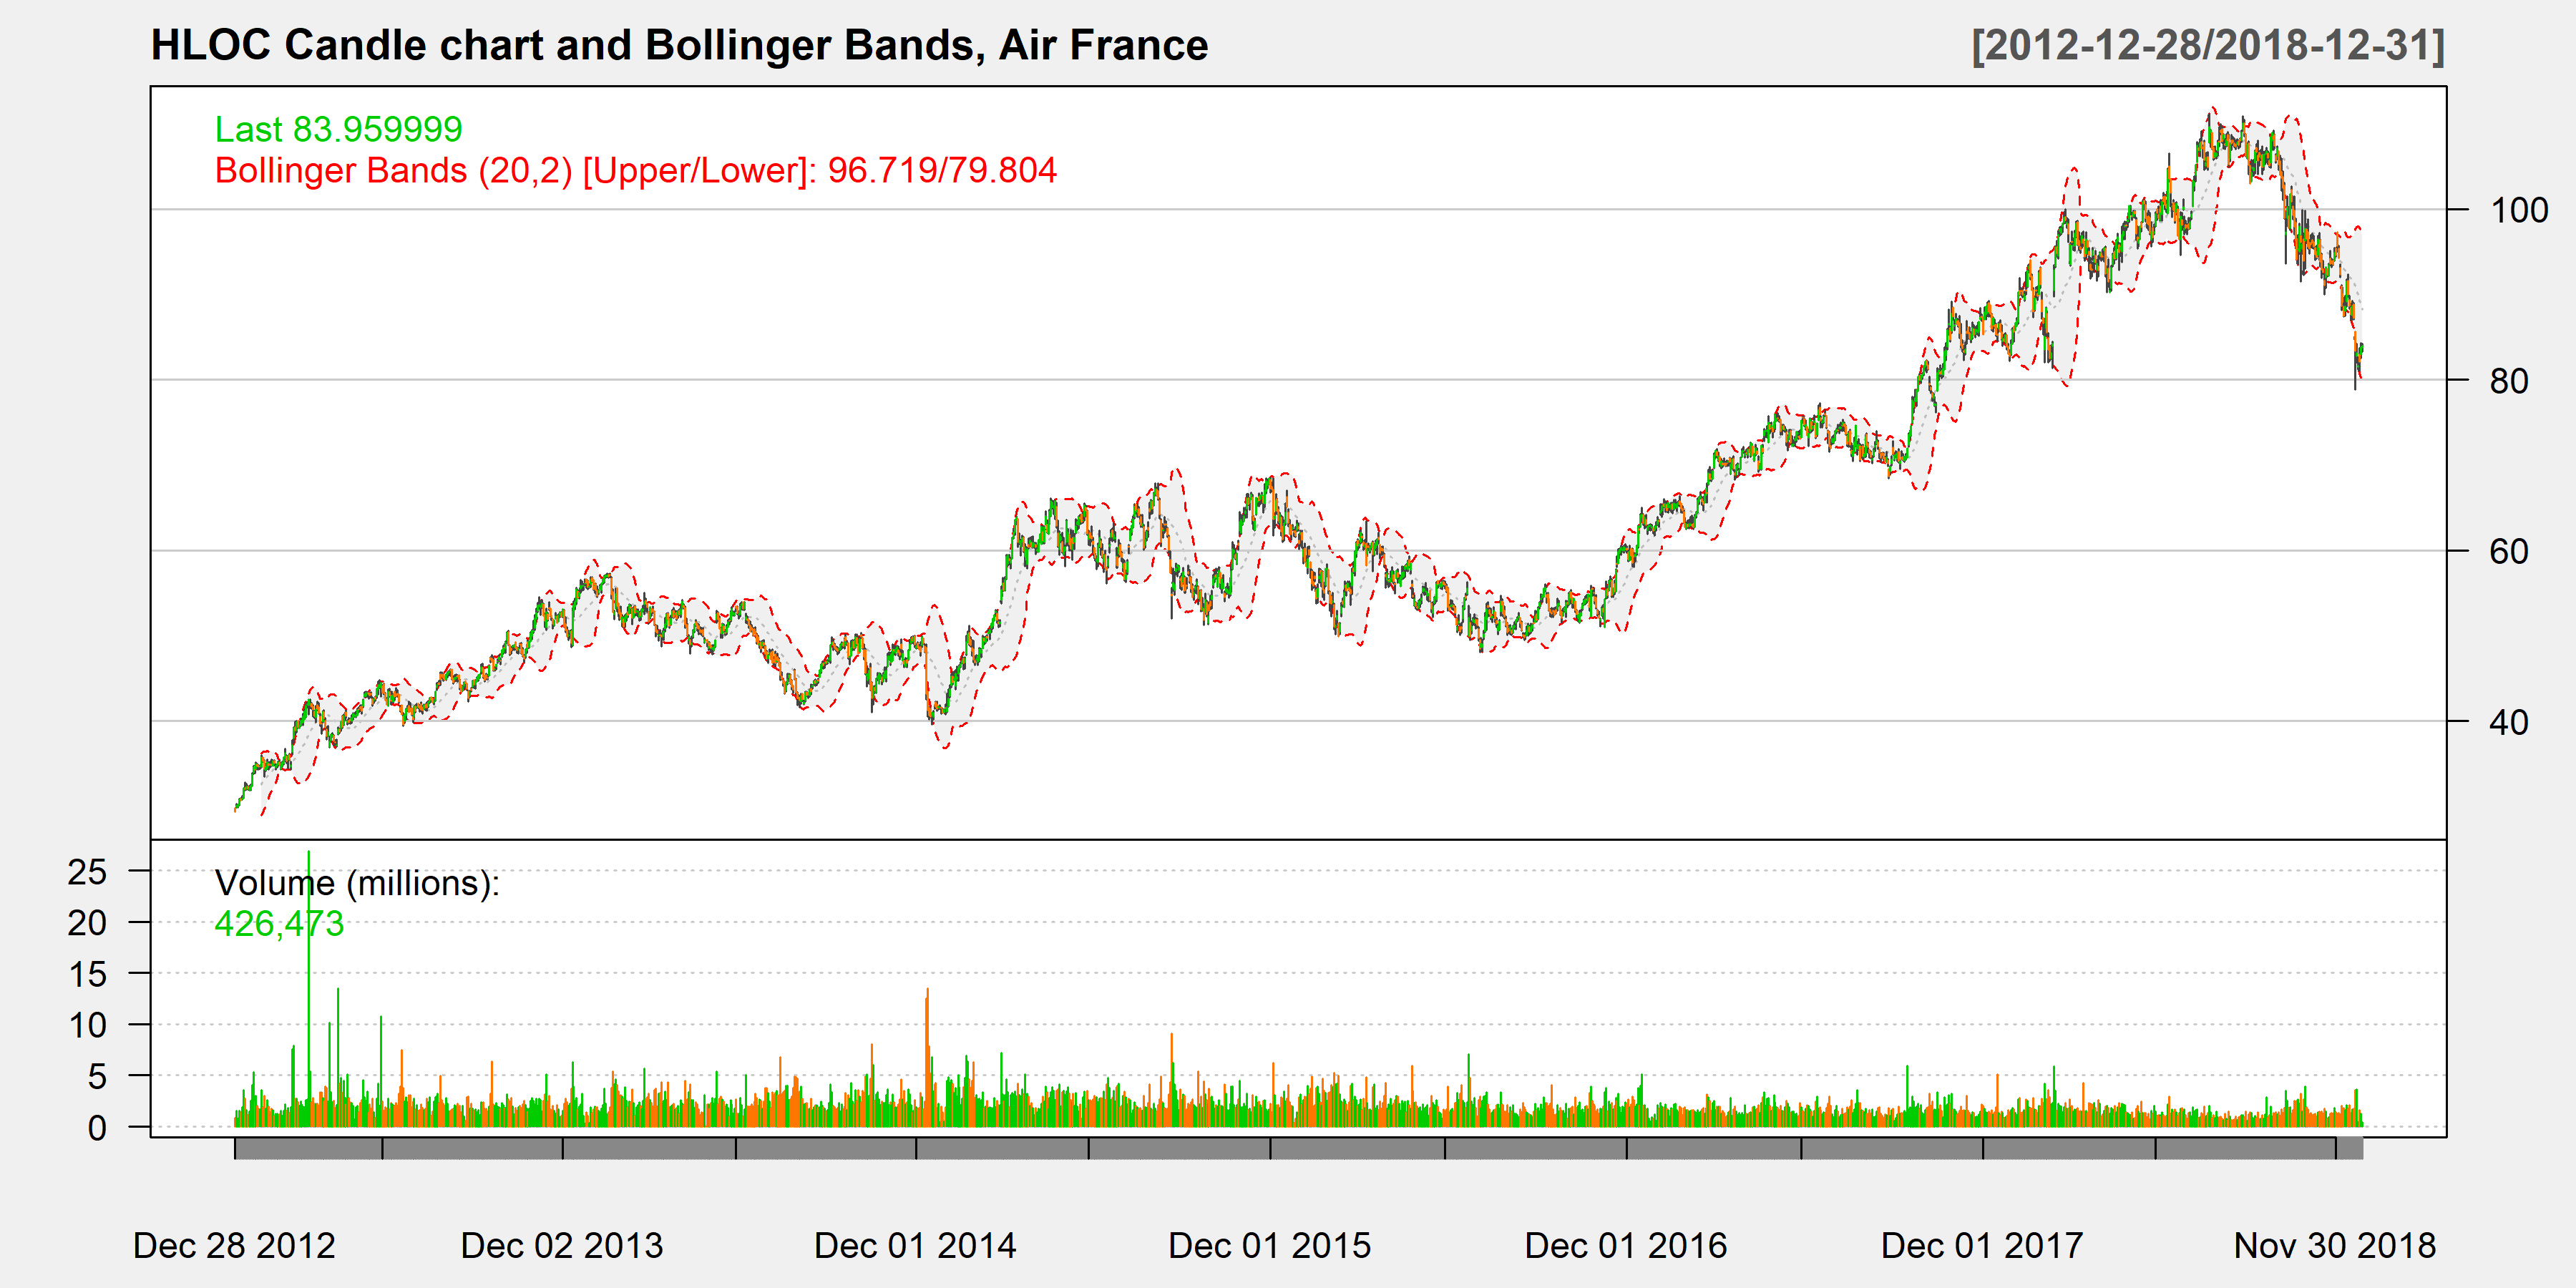
\includegraphics{"D:/2017-2018/data_analysis/technical_analysis/report/HLOC Candle chart and Bollinger Bands, Air France.png"}
\caption{Daily HLOC Chart price with Bollinger Bands (20,2)}
\end{figure}

\hypertarget{quantmod-blotter-and-quantstrat-packages}{%
\subsection{quantmod, blotter and quantstrat
packages}\label{quantmod-blotter-and-quantstrat-packages}}

One important building block towards the implementation of Technical
Analysis in R is the package quantmod \footnote{\url{https://github.com/joshuaulrich/quantmod}},
which allows the user to download stock prices data from Yahoo!, and to
visualize different types of price charts, which are of great support in
a first, rough analysis of the evolution of price trends over time. For
the sake of offering a visual understanding of TA indicators, these
functionalities were already exploited in the previuous paragraph, using
the functions \texttt{quantmod::getSymbols()} and
\texttt{quantmod::chartSeries}, along with \texttt{quantmod::addSMA},
\texttt{quantmod::addRSI}, and \texttt{quantmod::addBBands}.

Moreover, R supports a package named \texttt{quantstrat}, a
``transaction-oriented infrastructure for constructing trading systems
and simulation'' \footnote{\url{https://www.rdocumentation.org/packages/quantstrat/versions/0.16.6}}.
However, this package counts several dependencies, and therefore we'll
need our machine to be equipped with all these packages, as brilliantly
shown in \citet{Yu2019}.

\begin{Shaded}
\begin{Highlighting}[]
\KeywordTok{install.packages}\NormalTok{(}\StringTok{"quantmod"}\NormalTok{)}
\KeywordTok{install.packages}\NormalTok{(}\StringTok{"FinancialInstrument"}\NormalTok{)}
\KeywordTok{install.packages}\NormalTok{(}\StringTok{"PerformanceAnalytics"}\NormalTok{)}
\KeywordTok{install.packages}\NormalTok{(}\StringTok{"foreach"}\NormalTok{)}
\KeywordTok{install.packages}\NormalTok{(}\StringTok{"devtools"}\NormalTok{)}
\NormalTok{devtools}\OperatorTok{::}\KeywordTok{install_github}\NormalTok{(}\StringTok{"braverock/blotter"}\NormalTok{)}
\NormalTok{devtools}\OperatorTok{::}\KeywordTok{install_github}\NormalTok{(}\StringTok{"braverock/quanstrat"}\NormalTok{)}
\end{Highlighting}
\end{Shaded}

\hypertarget{portfolio-management-with-quantstrat}{%
\subsection{Portfolio management with
quantstrat}\label{portfolio-management-with-quantstrat}}

We build an actively managed portfolio made of the top five firms of the
French CAC40 using six years of price data, from 2012-12-28 to
2018-12-31, for a total of 1534 trading days. The choice of the stocks
fell simply on those we consider to be liquid enough, so that the chance
of observing large sudden jumps in prices is low. In fact, fluctuations
would negatively affect the TA predictive perfomance.

Starting with an initial capital of €100000, we will buy or sell 100
stocks of each equity, whenever some conditions on past prices are met.
These conditions are later referred to as \emph{signals}, and are linked
to the indicators whose mathematical essence is shown in the previuos
part. Our main purpose is to create a plausible setup that, upon further
improvements, can help an agent to infer some information on future
prices movements based on past prices analysis. We will deliberately
leave this model at a simplistic and unsophisticated stage, for the sake
of outlying its main basic features with clarity. Nevertheless, several
improvements would be needed before a proper real-life implementation.
We will mention them in the remaining of this chapter.

\hypertarget{preliminary-setup}{%
\subsubsection{Preliminary setup}\label{preliminary-setup}}

We first retrieve data from Yahoo! to the R global environment:

\begin{Shaded}
\begin{Highlighting}[]
\NormalTok{from =}\StringTok{"2012-12-28"}
\NormalTok{to =}\StringTok{"2018-12-31"}
\NormalTok{symbols =}\StringTok{ }\KeywordTok{c}\NormalTok{(}\StringTok{"MC.PA"}\NormalTok{,}\StringTok{"BN.PA"}\NormalTok{,}\StringTok{"AIR.PA"}\NormalTok{,}\StringTok{"BNP.PA"}\NormalTok{,}\StringTok{"DG.PA"}\NormalTok{ )}
\CommentTok{# the .PA label is needed to specify the Paris CAC40 stock exchange}
\NormalTok{quantmod}\OperatorTok{::}\KeywordTok{getSymbols}\NormalTok{(symbols,}
                     \DataTypeTok{from=}\NormalTok{from, }\DataTypeTok{to=}\NormalTok{to)}
\end{Highlighting}
\end{Shaded}

We then set up the strategy, the portfolio and the account objects:

\begin{Shaded}
\begin{Highlighting}[]
\NormalTok{initEq=}\DecValTok{100000} \CommentTok{# capital to invest}

\NormalTok{strategy.st <-}\StringTok{ "strat.full.limit"} \CommentTok{# name the objects}
\NormalTok{portfolio.st <-}\StringTok{ "portf.full.limit"}
\NormalTok{account.st <-}\StringTok{ "acct.full.limit"}

\NormalTok{blotter}\OperatorTok{::}\KeywordTok{initPortf}\NormalTok{(portfolio.st, symbols) }\CommentTok{#initialize portfolio}
\NormalTok{blotter}\OperatorTok{::}\KeywordTok{initAcct}\NormalTok{(account.st, }\CommentTok{# need specifing also linked portfolio }
         \DataTypeTok{portfolios=}\NormalTok{portfolio.st, }
         \DataTypeTok{initEq =}\NormalTok{ initEq) }\CommentTok{# capital level}
\NormalTok{quantstrat}\OperatorTok{::}\KeywordTok{initOrders}\NormalTok{(portfolio.st) }\CommentTok{# the orders 'container'}
\NormalTok{quantstrat}\OperatorTok{::}\KeywordTok{strategy}\NormalTok{(strategy.st, }\DataTypeTok{store=}\OtherTok{TRUE}\NormalTok{) }\CommentTok{# save our strategy in }
\CommentTok{# the global environement}
\end{Highlighting}
\end{Shaded}

\hypertarget{creating-indicators}{%
\subsubsection{Creating indicators}\label{creating-indicators}}

As illustrated earlier, we make use of three simple indicators: simple
moving average, relative strength index and Bollinger Bands. The
indicators will be linked to the startegy object previoulsy defined. The
input dataframe is called \emph{mktdata}, an object that will be created
automatically when we validate the strategy.

\begin{Shaded}
\begin{Highlighting}[]
\NormalTok{quantstrat}\OperatorTok{::}\KeywordTok{add.indicator}\NormalTok{(}
\NormalTok{  strategy.st, }\DataTypeTok{name=}\StringTok{"SMA"}\NormalTok{, }\CommentTok{# "name" must correspond to an R function}
  \DataTypeTok{arguments=} \KeywordTok{list}\NormalTok{(}\DataTypeTok{x=} \KeywordTok{quote}\NormalTok{(}\KeywordTok{Cl}\NormalTok{(mktdata)), }\DataTypeTok{n=}\DecValTok{50}\NormalTok{), }\CommentTok{# input data are closing prices}
  \CommentTok{# set input data (mktdata) and indicator parameters through function 'arguments'}
  \DataTypeTok{label=}\StringTok{"sma50"}\NormalTok{) }\CommentTok{## unique reference 'mktdata' column name}

\KeywordTok{add.indicator}\NormalTok{(}\DataTypeTok{strategy =}\NormalTok{ strategy.st,}
              \DataTypeTok{name =} \StringTok{'RSI'}\NormalTok{, }\CommentTok{# normally, we'll be using functions }
              \CommentTok{# from the TTR package }
              \DataTypeTok{arguments =} \KeywordTok{list}\NormalTok{(}\DataTypeTok{price =} \KeywordTok{quote}\NormalTok{(}\KeywordTok{Cl}\NormalTok{(mktdata)), }\DataTypeTok{n=}\DecValTok{14}\NormalTok{), }
              \CommentTok{# among the 'arguments', we need to set the }
              \CommentTok{# parameter (number of days of the SMA) for the RSI}
              \DataTypeTok{label =} \StringTok{'rsi.14'}\NormalTok{)}

\KeywordTok{add.indicator}\NormalTok{(}\DataTypeTok{strategy =}\NormalTok{ strategy.st,}
              \DataTypeTok{name=} \StringTok{"BBands"}\NormalTok{, }
              \DataTypeTok{arguments =} 
                \KeywordTok{list}\NormalTok{(}\DataTypeTok{HLC =} \KeywordTok{quote}\NormalTok{(}\KeywordTok{HLC}\NormalTok{(mktdata)),}\DataTypeTok{n=}\DecValTok{20}\NormalTok{, }\DataTypeTok{maType=} \StringTok{"SMA"}\NormalTok{, }\DataTypeTok{sd=}\DecValTok{2}\NormalTok{), }
              \CommentTok{# BBands need High,Low and Closing Prices as an Input}
              \DataTypeTok{label =} \StringTok{"bb.20.2"}\NormalTok{)}
\end{Highlighting}
\end{Shaded}

\hypertarget{combining-indicators-to-create-trading-signals}{%
\subsubsection{Combining indicators to create trading
signals}\label{combining-indicators-to-create-trading-signals}}

The third step, after setting up the blotter objects and creating the
indicators, is creating buy and sell signals out of an appropriate blend
of indicators. Below we offer a summary of the signals that will be used
here.

\begin{longtable}[]{@{}lll@{}}
\caption{Summary of signals and related trading
executions}\tabularnewline
\toprule
\begin{minipage}[b]{0.30\columnwidth}\raggedright
Type of Signal\strut
\end{minipage} & \begin{minipage}[b]{0.42\columnwidth}\raggedright
Signal\strut
\end{minipage} & \begin{minipage}[b]{0.15\columnwidth}\raggedright
Execution\strut
\end{minipage}\tabularnewline
\midrule
\endfirsthead
\toprule
\begin{minipage}[b]{0.30\columnwidth}\raggedright
Type of Signal\strut
\end{minipage} & \begin{minipage}[b]{0.42\columnwidth}\raggedright
Signal\strut
\end{minipage} & \begin{minipage}[b]{0.15\columnwidth}\raggedright
Execution\strut
\end{minipage}\tabularnewline
\midrule
\endhead
\begin{minipage}[t]{0.30\columnwidth}\raggedright
Crossover\strut
\end{minipage} & \begin{minipage}[t]{0.42\columnwidth}\raggedright
SMA(50)\textgreater SMA(200)\strut
\end{minipage} & \begin{minipage}[t]{0.15\columnwidth}\raggedright
NA\strut
\end{minipage}\tabularnewline
\begin{minipage}[t]{0.30\columnwidth}\raggedright
Crossover\strut
\end{minipage} & \begin{minipage}[t]{0.42\columnwidth}\raggedright
SMA(50)\textless SMA(200)\strut
\end{minipage} & \begin{minipage}[t]{0.15\columnwidth}\raggedright
NA\strut
\end{minipage}\tabularnewline
\begin{minipage}[t]{0.30\columnwidth}\raggedright
Threshold\strut
\end{minipage} & \begin{minipage}[t]{0.42\columnwidth}\raggedright
RSI\textless30\strut
\end{minipage} & \begin{minipage}[t]{0.15\columnwidth}\raggedright
NA\strut
\end{minipage}\tabularnewline
\begin{minipage}[t]{0.30\columnwidth}\raggedright
Threshold\strut
\end{minipage} & \begin{minipage}[t]{0.42\columnwidth}\raggedright
RSI\textgreater70\strut
\end{minipage} & \begin{minipage}[t]{0.15\columnwidth}\raggedright
NA\strut
\end{minipage}\tabularnewline
\begin{minipage}[t]{0.30\columnwidth}\raggedright
Crossover \& Threshold\strut
\end{minipage} & \begin{minipage}[t]{0.42\columnwidth}\raggedright
SMA(50)\textgreater SMA(200) \& RSI\textless30\strut
\end{minipage} & \begin{minipage}[t]{0.15\columnwidth}\raggedright
BUY\strut
\end{minipage}\tabularnewline
\begin{minipage}[t]{0.30\columnwidth}\raggedright
Crossover \& Threshold\strut
\end{minipage} & \begin{minipage}[t]{0.42\columnwidth}\raggedright
SMA(50)\textless SMA(200) \& RSI\textgreater70\strut
\end{minipage} & \begin{minipage}[t]{0.15\columnwidth}\raggedright
SELL\strut
\end{minipage}\tabularnewline
\begin{minipage}[t]{0.30\columnwidth}\raggedright
Crossover\strut
\end{minipage} & \begin{minipage}[t]{0.42\columnwidth}\raggedright
Closing \textgreater{} Upper BBand\strut
\end{minipage} & \begin{minipage}[t]{0.15\columnwidth}\raggedright
NA\strut
\end{minipage}\tabularnewline
\begin{minipage}[t]{0.30\columnwidth}\raggedright
Crossover\strut
\end{minipage} & \begin{minipage}[t]{0.42\columnwidth}\raggedright
Closing \textless{} Lower BBand\strut
\end{minipage} & \begin{minipage}[t]{0.15\columnwidth}\raggedright
NA\strut
\end{minipage}\tabularnewline
\begin{minipage}[t]{0.30\columnwidth}\raggedright
Crossover \& Threshold\strut
\end{minipage} & \begin{minipage}[t]{0.42\columnwidth}\raggedright
Closing \textless{} Lower BBand \& RSI\textless30\strut
\end{minipage} & \begin{minipage}[t]{0.15\columnwidth}\raggedright
BUY\strut
\end{minipage}\tabularnewline
\begin{minipage}[t]{0.30\columnwidth}\raggedright
Crossover \& Threshold\strut
\end{minipage} & \begin{minipage}[t]{0.42\columnwidth}\raggedright
Closing \textgreater{} Upper BBand \& RSI\textgreater70\strut
\end{minipage} & \begin{minipage}[t]{0.15\columnwidth}\raggedright
SELL\strut
\end{minipage}\tabularnewline
\bottomrule
\end{longtable}

Despite having defined ten signals, only four of these will trigger
actual execution orders. This is because it looks safer to rely on a
mixed signal - i.e.~one making use of more than one indicator - rather
than only on a simple one.

Here is some code showing how a mixed signal is created, based on the
evaluation of two simple ones, which in turn may have different level of
complexities, depending on the kind of indicators used to build them.
Notice that the function \texttt{sigFormula} can take more than two
arguments, evaluating therefore several conditions at once.

\begin{Shaded}
\begin{Highlighting}[]
\CommentTok{## 'Bull market' (i.e. market considered underpriced --> indication to buy) }
\CommentTok{# if SMA50>SMA200}
\NormalTok{quantstrat}\OperatorTok{::}\KeywordTok{add.signal}\NormalTok{(}
\NormalTok{  strategy.st, }\DataTypeTok{name=}\StringTok{"sigCrossover"}\NormalTok{, }\CommentTok{## "name" is a function taking on}
           \CommentTok{# specific arguments }
           \DataTypeTok{arguments=} \KeywordTok{list}\NormalTok{(}\DataTypeTok{columns=}\KeywordTok{c}\NormalTok{(}\StringTok{"sma50"}\NormalTok{,}\StringTok{"sma200"}\NormalTok{),}\DataTypeTok{relationship=}\StringTok{"gt"}\NormalTok{), }
            \CommentTok{# 'columns' refers to the indicators defined above}
           \DataTypeTok{label=}\StringTok{"smabuy"}\NormalTok{) }\CommentTok{# 'label' will be the reference for }
\CommentTok{# the execution phase hereafter.}

\CommentTok{## Specifies all instance when RSI is below 30 }
\CommentTok{## (indication of asset being oversold)}
\KeywordTok{add.signal}\NormalTok{(strategy.st, }\DataTypeTok{name =} \StringTok{"sigThreshold"}\NormalTok{,}
           \DataTypeTok{arguments =} 
             \KeywordTok{list}\NormalTok{(}\DataTypeTok{column =} \StringTok{"rsi.14"}\NormalTok{, }\DataTypeTok{threshold =} \DecValTok{30}\NormalTok{, }\DataTypeTok{relationship =} \StringTok{"lt"}\NormalTok{, }
                  \DataTypeTok{cross =} \OtherTok{TRUE}\NormalTok{), }\CommentTok{# signals }
           \DataTypeTok{label =} \StringTok{"rsi14buy"}\NormalTok{)}

\CommentTok{## sigFormula which indicates that both smabuy and rsi14buy must evaluate TRUE.}
\KeywordTok{add.signal}\NormalTok{(strategy.st, }\DataTypeTok{name =} \StringTok{"sigFormula"}\NormalTok{,}
           \DataTypeTok{arguments =} \KeywordTok{list}\NormalTok{(}\DataTypeTok{formula =} \StringTok{"smabuy & rsi14buy"}\NormalTok{,}\DataTypeTok{cross =} \OtherTok{TRUE}\NormalTok{),}
           \CommentTok{# notice that the formula is evaluating two booleans }
           \DataTypeTok{label =} \StringTok{"entry1"}\NormalTok{) }
\end{Highlighting}
\end{Shaded}

\hypertarget{executing-tradings}{%
\subsubsection{Executing tradings}\label{executing-tradings}}

The very last step of our strategy will be defining the trading
operations to execute, once the relevant signals are observed. As shown
in Table 4, only four signals trigger an order execution. We define
accordingly four trading execution rules.

\begin{Shaded}
\begin{Highlighting}[]
\CommentTok{## Enter the position when SMA(50)>SMA(200), and the RSI<30}
\NormalTok{quantstrat}\OperatorTok{::}\KeywordTok{add.rule}\NormalTok{(}
\NormalTok{  strategy.st, }\DataTypeTok{name =} \StringTok{"ruleSignal"}\NormalTok{,}
         \DataTypeTok{arguments =} \KeywordTok{list}\NormalTok{(}\DataTypeTok{sigcol =} \StringTok{"entry1"}\NormalTok{, }\DataTypeTok{sigval =} \OtherTok{TRUE}\NormalTok{,}
                          \DataTypeTok{orderqty =} \DecValTok{1000}\NormalTok{, }\DataTypeTok{ordertype =} \StringTok{"market"}\NormalTok{,}
                          \DataTypeTok{orderside =} \StringTok{"long"}\NormalTok{, }\DataTypeTok{replace =} \OtherTok{FALSE}\NormalTok{,}
                          \DataTypeTok{prefer =} \StringTok{"Open"}\NormalTok{, }
                          \DataTypeTok{tradeSize =}\NormalTok{ tradesize, }\DataTypeTok{maxSize =}\NormalTok{ tradesize),}
         \DataTypeTok{type =} \StringTok{"enter"}\NormalTok{)  }


\CommentTok{## Exit the position when SMA(50)<SMA(200), and the RSI>70}
\KeywordTok{add.rule}\NormalTok{(strategy.st, }\DataTypeTok{name =} \StringTok{"ruleSignal"}\NormalTok{,}
         \DataTypeTok{arguments =} \KeywordTok{list}\NormalTok{(}\DataTypeTok{sigcol =} \StringTok{"exit1"}\NormalTok{, }\DataTypeTok{sigval =} \OtherTok{TRUE}\NormalTok{,}
                          \DataTypeTok{orderqty =} \DecValTok{-1000}\NormalTok{ , }\DataTypeTok{ordertype =} \StringTok{"market"}\NormalTok{,}
                          \DataTypeTok{orderside =} \StringTok{"long"}\NormalTok{, }\DataTypeTok{replace =} \OtherTok{FALSE}\NormalTok{,}
                          \DataTypeTok{prefer =} \StringTok{"Open"}\NormalTok{, }
                          \DataTypeTok{tradeSize =}\NormalTok{ tradesize, }
                          \DataTypeTok{maxSize =}\NormalTok{ tradesize),}
         \DataTypeTok{type =} \StringTok{"exit"}\NormalTok{) }


\CommentTok{## Enter the position when (Closing price < Lower BBand) and RSI<30}
\KeywordTok{add.rule}\NormalTok{(}\DataTypeTok{strategy =}\NormalTok{ strategy.st, }\DataTypeTok{name=} \StringTok{'ruleSignal'}\NormalTok{,}
         \DataTypeTok{arguments =} \KeywordTok{list}\NormalTok{(}\DataTypeTok{sigcol =} \StringTok{"entry2"}\NormalTok{, }\DataTypeTok{sigval=} \OtherTok{TRUE}\NormalTok{,}
                          \DataTypeTok{orderqty =} \DecValTok{1000}\NormalTok{, }\DataTypeTok{ordertype=} \StringTok{'market'}\NormalTok{, }
                          \DataTypeTok{orderside=} \OtherTok{NULL}\NormalTok{,}\DataTypeTok{threshold=}\OtherTok{NULL}\NormalTok{ ), }
         \DataTypeTok{type=} \StringTok{"enter"}\NormalTok{)}


\CommentTok{## Exit the position when (Closing price > Upper BBand) and RSI>70  }
\KeywordTok{add.rule}\NormalTok{(}\DataTypeTok{strategy =}\NormalTok{ strategy.st, }\DataTypeTok{name=} \StringTok{'ruleSignal'}\NormalTok{,}
         \DataTypeTok{arguments =} \KeywordTok{list}\NormalTok{(}\DataTypeTok{sigcol =} \StringTok{"exit2"}\NormalTok{, }\DataTypeTok{sigval=} \OtherTok{TRUE}\NormalTok{,}
                          \DataTypeTok{orderqty =} \DecValTok{-1000}\NormalTok{, }\DataTypeTok{ordertype=} \StringTok{'market'}\NormalTok{, }\DataTypeTok{orderside=} \OtherTok{NULL}\NormalTok{,}
                          \DataTypeTok{threshold=}\OtherTok{NULL}\NormalTok{ ),  }
         \DataTypeTok{type=} \StringTok{"exit"}\NormalTok{)}
\end{Highlighting}
\end{Shaded}

\hypertarget{running-the-model}{%
\subsubsection{Running the model}\label{running-the-model}}

At this stage, we are ready to run our model. It is safer to check first
whether the code for the strategy we seek to implement is `bug-free'. To
do this, we run the \texttt{quantstrat::applyStrategy} command within
the \texttt{base::try} function, which allows to ``run an expression
that might fail and allow the user's code to handle error-recovery''
\footnote{\url{https://stat.ethz.ch/R-manual/R-devel/library/base/html/try.html}}.

\begin{Shaded}
\begin{Highlighting}[]
\NormalTok{testing_strat <-}\StringTok{ }\NormalTok{base}\OperatorTok{::}\KeywordTok{try}\NormalTok{( quantstrat}\OperatorTok{::}\KeywordTok{applyStrategy}\NormalTok{(strategy.st,}
                        \DataTypeTok{portfolios=}\NormalTok{portfolio.st ))}
\CommentTok{## try is a function in one of the basis R packages}

\CommentTok{## We test whether our entire startegy was coded correctly }
\end{Highlighting}
\end{Shaded}

\begin{verbatim}
## [1] "Set capital to 100,000 Euros "
## initalize portfolio: portf.fullinitalize account: acct.fullinitializie strategy: strat.full[1] "2013-02-20 00:00:00 AIR.PA -100 @ 36.25"
## [1] "2013-08-01 00:00:00 AIR.PA -100 @ 45.275002"
## [1] "2013-10-07 00:00:00 AIR.PA -100 @ 50.299999"
## [1] "2014-07-17 00:00:00 AIR.PA 100 @ 44.98"
## [1] "2014-09-05 00:00:00 AIR.PA -100 @ 49.189999"
## [1] "2015-01-26 00:00:00 AIR.PA -100 @ 50.139999"
## [1] "2015-02-19 00:00:00 AIR.PA -100 @ 51.990002"
## [1] "2015-03-02 00:00:00 AIR.PA -100 @ 56.09"
## [1] "2016-06-14 00:00:00 AIR.PA 100 @ 50.98"
## [1] "2016-06-17 00:00:00 AIR.PA 100 @ 50.830002"
## [1] "2016-12-14 00:00:00 AIR.PA -100 @ 62.400002"
## [1] "2016-12-16 00:00:00 AIR.PA -100 @ 64.18"
## [1] "2017-02-24 00:00:00 AIR.PA -100 @ 68.349998"
## [1] "2017-10-25 00:00:00 AIR.PA -100 @ 83.470001"
## [1] "2017-11-01 00:00:00 AIR.PA -100 @ 87.379997"
## [1] "2018-06-15 00:00:00 AIR.PA -100 @ 103.599998"
## [1] "2013-06-25 00:00:00 FP.PA 100 @ 36.294998"
## [1] "2013-08-26 00:00:00 FP.PA -100 @ 42"
## [1] "2013-08-29 00:00:00 FP.PA -100 @ 42.509998"
## [1] "2014-05-09 00:00:00 FP.PA -100 @ 52.259998"
## [1] "2014-10-16 00:00:00 FP.PA 100 @ 42.555"
## [1] "2017-07-10 00:00:00 FP.PA 100 @ 42.764999"
## [1] "2018-05-18 00:00:00 FP.PA -100 @ 54.48"
## [1] "2014-01-09 00:00:00 MC.PA 100 @ 122.949997"
## [1] "2014-04-11 00:00:00 MC.PA -100 @ 141.199997"
## [1] "2014-07-28 00:00:00 MC.PA 100 @ 131.550003"
## [1] "2014-11-24 00:00:00 MC.PA -100 @ 144.300003"
## [1] "2014-12-18 00:00:00 MC.PA 100 @ 130.25"
## [1] "2015-02-05 00:00:00 MC.PA -100 @ 153.5"
## [1] "2015-03-12 00:00:00 MC.PA -100 @ 170.600006"
## [1] "2016-07-28 00:00:00 MC.PA -100 @ 153.350006"
## [1] "2016-10-12 00:00:00 MC.PA -100 @ 164.350006"
## [1] "2016-10-17 00:00:00 MC.PA -100 @ 165.399994"
## [1] "2017-01-20 00:00:00 MC.PA -100 @ 190.949997"
## [1] "2017-03-20 00:00:00 MC.PA -100 @ 200"
## [1] "2017-04-03 00:00:00 MC.PA -100 @ 204.050003"
## [1] "2017-04-25 00:00:00 MC.PA -100 @ 223.149994"
## [1] "2017-10-27 00:00:00 MC.PA -100 @ 253.949997"
## [1] "2018-04-11 00:00:00 MC.PA -100 @ 278.25"
## [1] "2018-10-11 00:00:00 MC.PA 100 @ 261.950012"
## [1] "2013-01-30 00:00:00 OR.PA -100 @ 113.550003"
## [1] "2013-04-03 00:00:00 OR.PA -100 @ 127.300003"
## [1] "2018-02-09 00:00:00 OR.PA 100 @ 172.350006"
## [1] "2018-10-11 00:00:00 OR.PA 100 @ 187.600006"
## [1] "2013-04-03 00:00:00 SAN.PA -100 @ 80.050003"
## [1] "2013-11-07 00:00:00 SAN.PA -100 @ 78.660004"
## [1] "2014-10-16 00:00:00 SAN.PA 100 @ 78.800003"
## [1] "2014-10-29 00:00:00 SAN.PA 100 @ 71.150002"
## [1] "2015-02-16 00:00:00 SAN.PA -100 @ 85.720001"
## [1] "2015-02-20 00:00:00 SAN.PA -100 @ 87.389999"
## [1] "2015-02-24 00:00:00 SAN.PA -100 @ 88.75"
## [1] "2015-04-10 00:00:00 SAN.PA -100 @ 98.75"
## [1] "2016-06-15 00:00:00 SAN.PA 100 @ 68.110001"
## [1] "2016-11-10 00:00:00 SAN.PA -100 @ 76.980003"
## [1] "2017-04-05 00:00:00 SAN.PA -100 @ 85.43"
## [1] "2017-05-05 00:00:00 SAN.PA -100 @ 89.690002"
## [1] "2017-12-06 00:00:00 SAN.PA 100 @ 73.25"
## [1] "2018-07-05 00:00:00 SAN.PA -100 @ 72.440002"
## [1] "2018-08-01 00:00:00 SAN.PA -100 @ 75.599998"
\end{verbatim}

Since the strategy appears to run smoothly, we can update our portfolio
and account to register the transactions and variations in the level of
capital owned. We are now ready to extract the data on the performance,
in the form of summary statistics and charts. Unfortunately, it seems
that, due to an apparently still unfixed bug in the quantstrat package
\footnote{\url{https://github.com/braverock/quantstrat/issues/57}}, it
is not possible to export the strategy log. This is why we kept it
printed to screen, as a full output of the command that runs the
relevant strategy implementation script.

\hypertarget{performance-evaluation}{%
\subsubsection{Performance evaluation}\label{performance-evaluation}}

As summarized in the first line of Table 5, our strategy tested on a
five-year panel with five stocks seems `conservative', in that the
maximum number of tradings on a stock is 17 (for MC.PA), with an average
of roughly 12 across the five stocks. This may be due to the usage of
long-term SMAs, which incorporate a low level of volatility. As the
table below shows, for three out of five stocks, the strategy net
performance is negative. In particular, trading on LVHM register a loss
above €50000. On the other hand, the strategy yields a positive return
for Total and Sanofi. The lines ``Percent.Positive'' and
``Percent.Negative'', combined with ``Num.Trades'', gives an idea of how
many open positions were closed during the observed time frame, and if
the operation carried a positive or negative yield. By looking at the
transaction log, one can see that the strategy on both Air France was
particualry unsuccessful because several short positions were opened
(hence, with the `expectation' of a fall in the prices), and were
(forcibly) closed only `at the end of the world' i.e.~when we close the
account and the portfolio at the end of our observed period, after
prices had rather steadly surged. For LVHM we see a slightly different
story, in which the first three couples of operations are three
profitable buy and sell, after which the algorithms becomes inefficient
and determines the same pattern as AIR.PA to be observed. Sanofi looks
like the example of a successful implementation of our algorithm.

There are now some issues regarding our strategy that we would like to
highlight, and that would require further inspection and study:

\begin{itemize}
\item
  the first n days of observations (where n is the highest parameter
  value across all indicators making use of moving averages ) , should
  be left out. This is because during those n days only one out of two
  rules is implemented. This can clearly be source of biases. However,
  in this R framework , this option does not seem to be offered, since
  the input data is fed through the object \texttt{mktdata}, which is
  created automatically when applying the strategy;
\item
  no transaction fees are considered. Hence, any possible gain obtained
  by this strategy is in fact a gross profit;
\item
  the algorithm parameters were set by a `thumb-rule' type of choice,
  i.e.~no action was taken to determine whether any further restrictons
  were to be put in place to obtain a better strategy performance. For a
  better treatment on the code-related side of this matter, we refer the
  reader to \citet{Trice2016} for a reference to parameter optimization
  and backtesting ;
\item
  no in-depth study on the market conditions over the six years observed
  was made, neither on the specific stocks cases. Table 1 shows that the
  firms considered belong to four different industrial sectors - hence,
  some sector specificity may play a role in determining the evolution
  of prices;
\item
  there is clearly the need for some constraints that prevent opening an
  excessive number of short positions - especially when the algorithm
  returns signals contrasting with price trend.
\end{itemize}

One remark on Table 5: it is generated through
\texttt{blotter::tradeStats}, and its output cannot be truncated.
Moreover, the function developement seems unfinished, as one can notice
from the uncomplete description of the statistics \footnote{Full account
  of the statistics here:
  \url{https://rdrr.io/rforge/blotter/man/tradeStats.html}} .

\begin{longtable}[]{@{}cccccc@{}}
\caption{Startegy trading statistics}\tabularnewline
\toprule
\begin{minipage}[b]{0.24\columnwidth}\centering
Measure\strut
\end{minipage} & \begin{minipage}[b]{0.10\columnwidth}\centering
AIR.PA\strut
\end{minipage} & \begin{minipage}[b]{0.10\columnwidth}\centering
FP.PA\strut
\end{minipage} & \begin{minipage}[b]{0.12\columnwidth}\centering
MC.PA\strut
\end{minipage} & \begin{minipage}[b]{0.10\columnwidth}\centering
OR.PA\strut
\end{minipage} & \begin{minipage}[b]{0.10\columnwidth}\centering
SAN.PA\strut
\end{minipage}\tabularnewline
\midrule
\endfirsthead
\toprule
\begin{minipage}[b]{0.24\columnwidth}\centering
Measure\strut
\end{minipage} & \begin{minipage}[b]{0.10\columnwidth}\centering
AIR.PA\strut
\end{minipage} & \begin{minipage}[b]{0.10\columnwidth}\centering
FP.PA\strut
\end{minipage} & \begin{minipage}[b]{0.12\columnwidth}\centering
MC.PA\strut
\end{minipage} & \begin{minipage}[b]{0.10\columnwidth}\centering
OR.PA\strut
\end{minipage} & \begin{minipage}[b]{0.10\columnwidth}\centering
SAN.PA\strut
\end{minipage}\tabularnewline
\midrule
\endhead
\begin{minipage}[t]{0.24\columnwidth}\centering
Num.Txns\strut
\end{minipage} & \begin{minipage}[t]{0.10\columnwidth}\centering
16\strut
\end{minipage} & \begin{minipage}[t]{0.10\columnwidth}\centering
7\strut
\end{minipage} & \begin{minipage}[t]{0.12\columnwidth}\centering
17\strut
\end{minipage} & \begin{minipage}[t]{0.10\columnwidth}\centering
4\strut
\end{minipage} & \begin{minipage}[t]{0.10\columnwidth}\centering
15\strut
\end{minipage}\tabularnewline
\begin{minipage}[t]{0.24\columnwidth}\centering
Num.Trades\strut
\end{minipage} & \begin{minipage}[t]{0.10\columnwidth}\centering
1\strut
\end{minipage} & \begin{minipage}[t]{0.10\columnwidth}\centering
3\strut
\end{minipage} & \begin{minipage}[t]{0.12\columnwidth}\centering
4\strut
\end{minipage} & \begin{minipage}[t]{0.10\columnwidth}\centering
1\strut
\end{minipage} & \begin{minipage}[t]{0.10\columnwidth}\centering
2\strut
\end{minipage}\tabularnewline
\begin{minipage}[t]{0.24\columnwidth}\centering
Net.Trading.PL\strut
\end{minipage} & \begin{minipage}[t]{0.10\columnwidth}\centering
-17778\strut
\end{minipage} & \begin{minipage}[t]{0.10\columnwidth}\centering
2346\strut
\end{minipage} & \begin{minipage}[t]{0.12\columnwidth}\centering
-52745\strut
\end{minipage} & \begin{minipage}[t]{0.10\columnwidth}\centering
-11910\strut
\end{minipage} & \begin{minipage}[t]{0.10\columnwidth}\centering
9853\strut
\end{minipage}\tabularnewline
\begin{minipage}[t]{0.24\columnwidth}\centering
Avg.Trade.PL\strut
\end{minipage} & \begin{minipage}[t]{0.10\columnwidth}\centering
-17778\strut
\end{minipage} & \begin{minipage}[t]{0.10\columnwidth}\centering
781.8\strut
\end{minipage} & \begin{minipage}[t]{0.12\columnwidth}\centering
-13186\strut
\end{minipage} & \begin{minipage}[t]{0.10\columnwidth}\centering
-11910\strut
\end{minipage} & \begin{minipage}[t]{0.10\columnwidth}\centering
4926\strut
\end{minipage}\tabularnewline
\begin{minipage}[t]{0.24\columnwidth}\centering
Med.Trade.PL\strut
\end{minipage} & \begin{minipage}[t]{0.10\columnwidth}\centering
-17778\strut
\end{minipage} & \begin{minipage}[t]{0.10\columnwidth}\centering
830\strut
\end{minipage} & \begin{minipage}[t]{0.12\columnwidth}\centering
1550\strut
\end{minipage} & \begin{minipage}[t]{0.10\columnwidth}\centering
-11910\strut
\end{minipage} & \begin{minipage}[t]{0.10\columnwidth}\centering
4926\strut
\end{minipage}\tabularnewline
\begin{minipage}[t]{0.24\columnwidth}\centering
Largest.Winner\strut
\end{minipage} & \begin{minipage}[t]{0.10\columnwidth}\centering
0\strut
\end{minipage} & \begin{minipage}[t]{0.10\columnwidth}\centering
570.5\strut
\end{minipage} & \begin{minipage}[t]{0.12\columnwidth}\centering
2325\strut
\end{minipage} & \begin{minipage}[t]{0.10\columnwidth}\centering
0\strut
\end{minipage} & \begin{minipage}[t]{0.10\columnwidth}\centering
2204\strut
\end{minipage}\tabularnewline
\begin{minipage}[t]{0.24\columnwidth}\centering
Largest.Loser\strut
\end{minipage} & \begin{minipage}[t]{0.10\columnwidth}\centering
-176.4\strut
\end{minipage} & \begin{minipage}[t]{0.10\columnwidth}\centering
0\strut
\end{minipage} & \begin{minipage}[t]{0.12\columnwidth}\centering
-6154\strut
\end{minipage} & \begin{minipage}[t]{0.10\columnwidth}\centering
-6718\strut
\end{minipage} & \begin{minipage}[t]{0.10\columnwidth}\centering
0\strut
\end{minipage}\tabularnewline
\begin{minipage}[t]{0.24\columnwidth}\centering
Gross.Profits\strut
\end{minipage} & \begin{minipage}[t]{0.10\columnwidth}\centering
0\strut
\end{minipage} & \begin{minipage}[t]{0.10\columnwidth}\centering
2346\strut
\end{minipage} & \begin{minipage}[t]{0.12\columnwidth}\centering
5425\strut
\end{minipage} & \begin{minipage}[t]{0.10\columnwidth}\centering
0\strut
\end{minipage} & \begin{minipage}[t]{0.10\columnwidth}\centering
9853\strut
\end{minipage}\tabularnewline
\begin{minipage}[t]{0.24\columnwidth}\centering
Gross.Losses\strut
\end{minipage} & \begin{minipage}[t]{0.10\columnwidth}\centering
-17778\strut
\end{minipage} & \begin{minipage}[t]{0.10\columnwidth}\centering
0\strut
\end{minipage} & \begin{minipage}[t]{0.12\columnwidth}\centering
-58170\strut
\end{minipage} & \begin{minipage}[t]{0.10\columnwidth}\centering
-11910\strut
\end{minipage} & \begin{minipage}[t]{0.10\columnwidth}\centering
0\strut
\end{minipage}\tabularnewline
\begin{minipage}[t]{0.24\columnwidth}\centering
Std.Dev.Trade.PL\strut
\end{minipage} & \begin{minipage}[t]{0.10\columnwidth}\centering
NA\strut
\end{minipage} & \begin{minipage}[t]{0.10\columnwidth}\centering
191.8\strut
\end{minipage} & \begin{minipage}[t]{0.12\columnwidth}\centering
29992\strut
\end{minipage} & \begin{minipage}[t]{0.10\columnwidth}\centering
NA\strut
\end{minipage} & \begin{minipage}[t]{0.10\columnwidth}\centering
5728\strut
\end{minipage}\tabularnewline
\begin{minipage}[t]{0.24\columnwidth}\centering
Std.Err.Trade.PL\strut
\end{minipage} & \begin{minipage}[t]{0.10\columnwidth}\centering
NA\strut
\end{minipage} & \begin{minipage}[t]{0.10\columnwidth}\centering
110.8\strut
\end{minipage} & \begin{minipage}[t]{0.12\columnwidth}\centering
14996\strut
\end{minipage} & \begin{minipage}[t]{0.10\columnwidth}\centering
NA\strut
\end{minipage} & \begin{minipage}[t]{0.10\columnwidth}\centering
4050\strut
\end{minipage}\tabularnewline
\begin{minipage}[t]{0.24\columnwidth}\centering
Percent.Positive\strut
\end{minipage} & \begin{minipage}[t]{0.10\columnwidth}\centering
0\strut
\end{minipage} & \begin{minipage}[t]{0.10\columnwidth}\centering
100\strut
\end{minipage} & \begin{minipage}[t]{0.12\columnwidth}\centering
75\strut
\end{minipage} & \begin{minipage}[t]{0.10\columnwidth}\centering
0\strut
\end{minipage} & \begin{minipage}[t]{0.10\columnwidth}\centering
100\strut
\end{minipage}\tabularnewline
\begin{minipage}[t]{0.24\columnwidth}\centering
Percent.Negative\strut
\end{minipage} & \begin{minipage}[t]{0.10\columnwidth}\centering
100\strut
\end{minipage} & \begin{minipage}[t]{0.10\columnwidth}\centering
0\strut
\end{minipage} & \begin{minipage}[t]{0.12\columnwidth}\centering
25\strut
\end{minipage} & \begin{minipage}[t]{0.10\columnwidth}\centering
100\strut
\end{minipage} & \begin{minipage}[t]{0.10\columnwidth}\centering
0\strut
\end{minipage}\tabularnewline
\begin{minipage}[t]{0.24\columnwidth}\centering
Profit.Factor\strut
\end{minipage} & \begin{minipage}[t]{0.10\columnwidth}\centering
0\strut
\end{minipage} & \begin{minipage}[t]{0.10\columnwidth}\centering
NA\strut
\end{minipage} & \begin{minipage}[t]{0.12\columnwidth}\centering
0.09\strut
\end{minipage} & \begin{minipage}[t]{0.10\columnwidth}\centering
0\strut
\end{minipage} & \begin{minipage}[t]{0.10\columnwidth}\centering
NA\strut
\end{minipage}\tabularnewline
\begin{minipage}[t]{0.24\columnwidth}\centering
Avg.Win.Trade\strut
\end{minipage} & \begin{minipage}[t]{0.10\columnwidth}\centering
NA\strut
\end{minipage} & \begin{minipage}[t]{0.10\columnwidth}\centering
781.8\strut
\end{minipage} & \begin{minipage}[t]{0.12\columnwidth}\centering
1808\strut
\end{minipage} & \begin{minipage}[t]{0.10\columnwidth}\centering
NA\strut
\end{minipage} & \begin{minipage}[t]{0.10\columnwidth}\centering
4926\strut
\end{minipage}\tabularnewline
\begin{minipage}[t]{0.24\columnwidth}\centering
Med.Win.Trade\strut
\end{minipage} & \begin{minipage}[t]{0.10\columnwidth}\centering
NA\strut
\end{minipage} & \begin{minipage}[t]{0.10\columnwidth}\centering
830\strut
\end{minipage} & \begin{minipage}[t]{0.12\columnwidth}\centering
1825\strut
\end{minipage} & \begin{minipage}[t]{0.10\columnwidth}\centering
NA\strut
\end{minipage} & \begin{minipage}[t]{0.10\columnwidth}\centering
4926\strut
\end{minipage}\tabularnewline
\begin{minipage}[t]{0.24\columnwidth}\centering
Avg.Losing.Trade\strut
\end{minipage} & \begin{minipage}[t]{0.10\columnwidth}\centering
-17778\strut
\end{minipage} & \begin{minipage}[t]{0.10\columnwidth}\centering
NA\strut
\end{minipage} & \begin{minipage}[t]{0.12\columnwidth}\centering
-58170\strut
\end{minipage} & \begin{minipage}[t]{0.10\columnwidth}\centering
-11910\strut
\end{minipage} & \begin{minipage}[t]{0.10\columnwidth}\centering
NA\strut
\end{minipage}\tabularnewline
\begin{minipage}[t]{0.24\columnwidth}\centering
Med.Losing.Trade\strut
\end{minipage} & \begin{minipage}[t]{0.10\columnwidth}\centering
-17778\strut
\end{minipage} & \begin{minipage}[t]{0.10\columnwidth}\centering
NA\strut
\end{minipage} & \begin{minipage}[t]{0.12\columnwidth}\centering
-58170\strut
\end{minipage} & \begin{minipage}[t]{0.10\columnwidth}\centering
-11910\strut
\end{minipage} & \begin{minipage}[t]{0.10\columnwidth}\centering
NA\strut
\end{minipage}\tabularnewline
\begin{minipage}[t]{0.24\columnwidth}\centering
Avg.Daily.PL\strut
\end{minipage} & \begin{minipage}[t]{0.10\columnwidth}\centering
-147.2\strut
\end{minipage} & \begin{minipage}[t]{0.10\columnwidth}\centering
505.2\strut
\end{minipage} & \begin{minipage}[t]{0.12\columnwidth}\centering
-182.4\strut
\end{minipage} & \begin{minipage}[t]{0.10\columnwidth}\centering
-5955\strut
\end{minipage} & \begin{minipage}[t]{0.10\columnwidth}\centering
1116\strut
\end{minipage}\tabularnewline
\begin{minipage}[t]{0.24\columnwidth}\centering
Med.Daily.PL\strut
\end{minipage} & \begin{minipage}[t]{0.10\columnwidth}\centering
-161.4\strut
\end{minipage} & \begin{minipage}[t]{0.10\columnwidth}\centering
483\strut
\end{minipage} & \begin{minipage}[t]{0.12\columnwidth}\centering
1550\strut
\end{minipage} & \begin{minipage}[t]{0.10\columnwidth}\centering
-5955\strut
\end{minipage} & \begin{minipage}[t]{0.10\columnwidth}\centering
1102\strut
\end{minipage}\tabularnewline
\begin{minipage}[t]{0.24\columnwidth}\centering
Std.Dev.Daily.PL\strut
\end{minipage} & \begin{minipage}[t]{0.10\columnwidth}\centering
38.33\strut
\end{minipage} & \begin{minipage}[t]{0.10\columnwidth}\centering
57.55\strut
\end{minipage} & \begin{minipage}[t]{0.12\columnwidth}\centering
4004\strut
\end{minipage} & \begin{minipage}[t]{0.10\columnwidth}\centering
1078\strut
\end{minipage} & \begin{minipage}[t]{0.10\columnwidth}\centering
907.1\strut
\end{minipage}\tabularnewline
\begin{minipage}[t]{0.24\columnwidth}\centering
Std.Err.Daily.PL\strut
\end{minipage} & \begin{minipage}[t]{0.10\columnwidth}\centering
22.13\strut
\end{minipage} & \begin{minipage}[t]{0.10\columnwidth}\centering
33.22\strut
\end{minipage} & \begin{minipage}[t]{0.12\columnwidth}\centering
2002\strut
\end{minipage} & \begin{minipage}[t]{0.10\columnwidth}\centering
762.5\strut
\end{minipage} & \begin{minipage}[t]{0.10\columnwidth}\centering
453.5\strut
\end{minipage}\tabularnewline
\begin{minipage}[t]{0.24\columnwidth}\centering
Ann.Sharpe\strut
\end{minipage} & \begin{minipage}[t]{0.10\columnwidth}\centering
-60.98\strut
\end{minipage} & \begin{minipage}[t]{0.10\columnwidth}\centering
139.3\strut
\end{minipage} & \begin{minipage}[t]{0.12\columnwidth}\centering
-0.72\strut
\end{minipage} & \begin{minipage}[t]{0.10\columnwidth}\centering
-87.67\strut
\end{minipage} & \begin{minipage}[t]{0.10\columnwidth}\centering
19.53\strut
\end{minipage}\tabularnewline
\begin{minipage}[t]{0.24\columnwidth}\centering
Max.Drawdown\strut
\end{minipage} & \begin{minipage}[t]{0.10\columnwidth}\centering
-45318\strut
\end{minipage} & \begin{minipage}[t]{0.10\columnwidth}\centering
-1522\strut
\end{minipage} & \begin{minipage}[t]{0.12\columnwidth}\centering
-115215\strut
\end{minipage} & \begin{minipage}[t]{0.10\columnwidth}\centering
-16030\strut
\end{minipage} & \begin{minipage}[t]{0.10\columnwidth}\centering
-10475\strut
\end{minipage}\tabularnewline
\begin{minipage}[t]{0.24\columnwidth}\centering
Profit.To.Max.Draw\strut
\end{minipage} & \begin{minipage}[t]{0.10\columnwidth}\centering
-0.39\strut
\end{minipage} & \begin{minipage}[t]{0.10\columnwidth}\centering
1.54\strut
\end{minipage} & \begin{minipage}[t]{0.12\columnwidth}\centering
-0.46\strut
\end{minipage} & \begin{minipage}[t]{0.10\columnwidth}\centering
-0.74\strut
\end{minipage} & \begin{minipage}[t]{0.10\columnwidth}\centering
0.94\strut
\end{minipage}\tabularnewline
\begin{minipage}[t]{0.24\columnwidth}\centering
Avg.WinLoss.Ratio\strut
\end{minipage} & \begin{minipage}[t]{0.10\columnwidth}\centering
NA\strut
\end{minipage} & \begin{minipage}[t]{0.10\columnwidth}\centering
NA\strut
\end{minipage} & \begin{minipage}[t]{0.12\columnwidth}\centering
0.03\strut
\end{minipage} & \begin{minipage}[t]{0.10\columnwidth}\centering
NA\strut
\end{minipage} & \begin{minipage}[t]{0.10\columnwidth}\centering
NA\strut
\end{minipage}\tabularnewline
\begin{minipage}[t]{0.24\columnwidth}\centering
Med.WinLoss.Ratio\strut
\end{minipage} & \begin{minipage}[t]{0.10\columnwidth}\centering
NA\strut
\end{minipage} & \begin{minipage}[t]{0.10\columnwidth}\centering
NA\strut
\end{minipage} & \begin{minipage}[t]{0.12\columnwidth}\centering
0.03\strut
\end{minipage} & \begin{minipage}[t]{0.10\columnwidth}\centering
NA\strut
\end{minipage} & \begin{minipage}[t]{0.10\columnwidth}\centering
NA\strut
\end{minipage}\tabularnewline
\begin{minipage}[t]{0.24\columnwidth}\centering
Max.Equity\strut
\end{minipage} & \begin{minipage}[t]{0.10\columnwidth}\centering
1440\strut
\end{minipage} & \begin{minipage}[t]{0.10\columnwidth}\centering
2440\strut
\end{minipage} & \begin{minipage}[t]{0.12\columnwidth}\centering
9345\strut
\end{minipage} & \begin{minipage}[t]{0.10\columnwidth}\centering
1045\strut
\end{minipage} & \begin{minipage}[t]{0.10\columnwidth}\centering
16406\strut
\end{minipage}\tabularnewline
\begin{minipage}[t]{0.24\columnwidth}\centering
Min.Equity\strut
\end{minipage} & \begin{minipage}[t]{0.10\columnwidth}\centering
-43878\strut
\end{minipage} & \begin{minipage}[t]{0.10\columnwidth}\centering
-856.5\strut
\end{minipage} & \begin{minipage}[t]{0.12\columnwidth}\centering
-105870\strut
\end{minipage} & \begin{minipage}[t]{0.10\columnwidth}\centering
-14985\strut
\end{minipage} & \begin{minipage}[t]{0.10\columnwidth}\centering
-3323\strut
\end{minipage}\tabularnewline
\begin{minipage}[t]{0.24\columnwidth}\centering
End.Equity\strut
\end{minipage} & \begin{minipage}[t]{0.10\columnwidth}\centering
-17778\strut
\end{minipage} & \begin{minipage}[t]{0.10\columnwidth}\centering
2346\strut
\end{minipage} & \begin{minipage}[t]{0.12\columnwidth}\centering
-52745\strut
\end{minipage} & \begin{minipage}[t]{0.10\columnwidth}\centering
-11910\strut
\end{minipage} & \begin{minipage}[t]{0.10\columnwidth}\centering
9853\strut
\end{minipage}\tabularnewline
\bottomrule
\end{longtable}

As one could have speculated by looking at the strategy log, only FP.PA
and SAN.PA yield a positive return, under the active strategy we
implemented. On the other hand, the three other stocks yield a negative
return, with MC.PA being the worst among the three.

A quick glance at the risk measure indicator seems to suggest that a
high volatility may have an implication on the accuracy of our automated
trading strategy - indeed, AIR.PA and MC.PA were traded unprofitably,
and their standard deviation is the highest. One may guess that the
algorithm was thrown off by the frequent changes in prices. There is
clearly the need for a more thorough analysis of these statistics, which
however goes beyond the scope of our analysis.

\begin{longtable}[]{@{}cccccc@{}}
\caption{Active strategy returns' statistics}\tabularnewline
\toprule
\begin{minipage}[b]{0.18\columnwidth}\centering
Measure\strut
\end{minipage} & \begin{minipage}[b]{0.13\columnwidth}\centering
AIR.PA DailyEqPL\strut
\end{minipage} & \begin{minipage}[b]{0.13\columnwidth}\centering
FP.PA DailyEqPL\strut
\end{minipage} & \begin{minipage}[b]{0.13\columnwidth}\centering
MC.PA DailyEqPL\strut
\end{minipage} & \begin{minipage}[b]{0.13\columnwidth}\centering
OR.PA DailyEqPL\strut
\end{minipage} & \begin{minipage}[b]{0.13\columnwidth}\centering
SAN.PA DailyEqPL\strut
\end{minipage}\tabularnewline
\midrule
\endfirsthead
\toprule
\begin{minipage}[b]{0.18\columnwidth}\centering
Measure\strut
\end{minipage} & \begin{minipage}[b]{0.13\columnwidth}\centering
AIR.PA DailyEqPL\strut
\end{minipage} & \begin{minipage}[b]{0.13\columnwidth}\centering
FP.PA DailyEqPL\strut
\end{minipage} & \begin{minipage}[b]{0.13\columnwidth}\centering
MC.PA DailyEqPL\strut
\end{minipage} & \begin{minipage}[b]{0.13\columnwidth}\centering
OR.PA DailyEqPL\strut
\end{minipage} & \begin{minipage}[b]{0.13\columnwidth}\centering
SAN.PA DailyEqPL\strut
\end{minipage}\tabularnewline
\midrule
\endhead
\begin{minipage}[t]{0.18\columnwidth}\centering
Cumulative Return\strut
\end{minipage} & \begin{minipage}[t]{0.13\columnwidth}\centering
-0.202\strut
\end{minipage} & \begin{minipage}[t]{0.13\columnwidth}\centering
0.023\strut
\end{minipage} & \begin{minipage}[t]{0.13\columnwidth}\centering
-0.55\strut
\end{minipage} & \begin{minipage}[t]{0.13\columnwidth}\centering
-0.121\strut
\end{minipage} & \begin{minipage}[t]{0.13\columnwidth}\centering
0.09\strut
\end{minipage}\tabularnewline
\begin{minipage}[t]{0.18\columnwidth}\centering
Annualized Return\strut
\end{minipage} & \begin{minipage}[t]{0.13\columnwidth}\centering
-0.036\strut
\end{minipage} & \begin{minipage}[t]{0.13\columnwidth}\centering
0.004\strut
\end{minipage} & \begin{minipage}[t]{0.13\columnwidth}\centering
-0.123\strut
\end{minipage} & \begin{minipage}[t]{0.13\columnwidth}\centering
-0.021\strut
\end{minipage} & \begin{minipage}[t]{0.13\columnwidth}\centering
0.014\strut
\end{minipage}\tabularnewline
\begin{minipage}[t]{0.18\columnwidth}\centering
Annualized Sharpe Ratio\strut
\end{minipage} & \begin{minipage}[t]{0.13\columnwidth}\centering
-0.291\strut
\end{minipage} & \begin{minipage}[t]{0.13\columnwidth}\centering
0.35\strut
\end{minipage} & \begin{minipage}[t]{0.13\columnwidth}\centering
-0.411\strut
\end{minipage} & \begin{minipage}[t]{0.13\columnwidth}\centering
-0.372\strut
\end{minipage} & \begin{minipage}[t]{0.13\columnwidth}\centering
0.228\strut
\end{minipage}\tabularnewline
\begin{minipage}[t]{0.18\columnwidth}\centering
Annualized StdDev\strut
\end{minipage} & \begin{minipage}[t]{0.13\columnwidth}\centering
0.125\strut
\end{minipage} & \begin{minipage}[t]{0.13\columnwidth}\centering
0.011\strut
\end{minipage} & \begin{minipage}[t]{0.13\columnwidth}\centering
0.299\strut
\end{minipage} & \begin{minipage}[t]{0.13\columnwidth}\centering
0.056\strut
\end{minipage} & \begin{minipage}[t]{0.13\columnwidth}\centering
0.063\strut
\end{minipage}\tabularnewline
\bottomrule
\end{longtable}

Finally, we consider one very last measure of ``fitness'' of our
startegy, which is by far the simplest: the level of capital left in our
account, once all positions have been closed. We see from Figure 4 that
the initial capital of €100000 has decreased to below €50000 (or
\(5e+04\)). Moreover, there seems to be the need for a constraint on the
capital invested, since towards the end of the observed period, one
would actually get indebted. To our knowledge, one should hard-code an
appropriate function to prevent more short positions being taken once
the level of capital goes below zero.

\begin{figure}
\centering
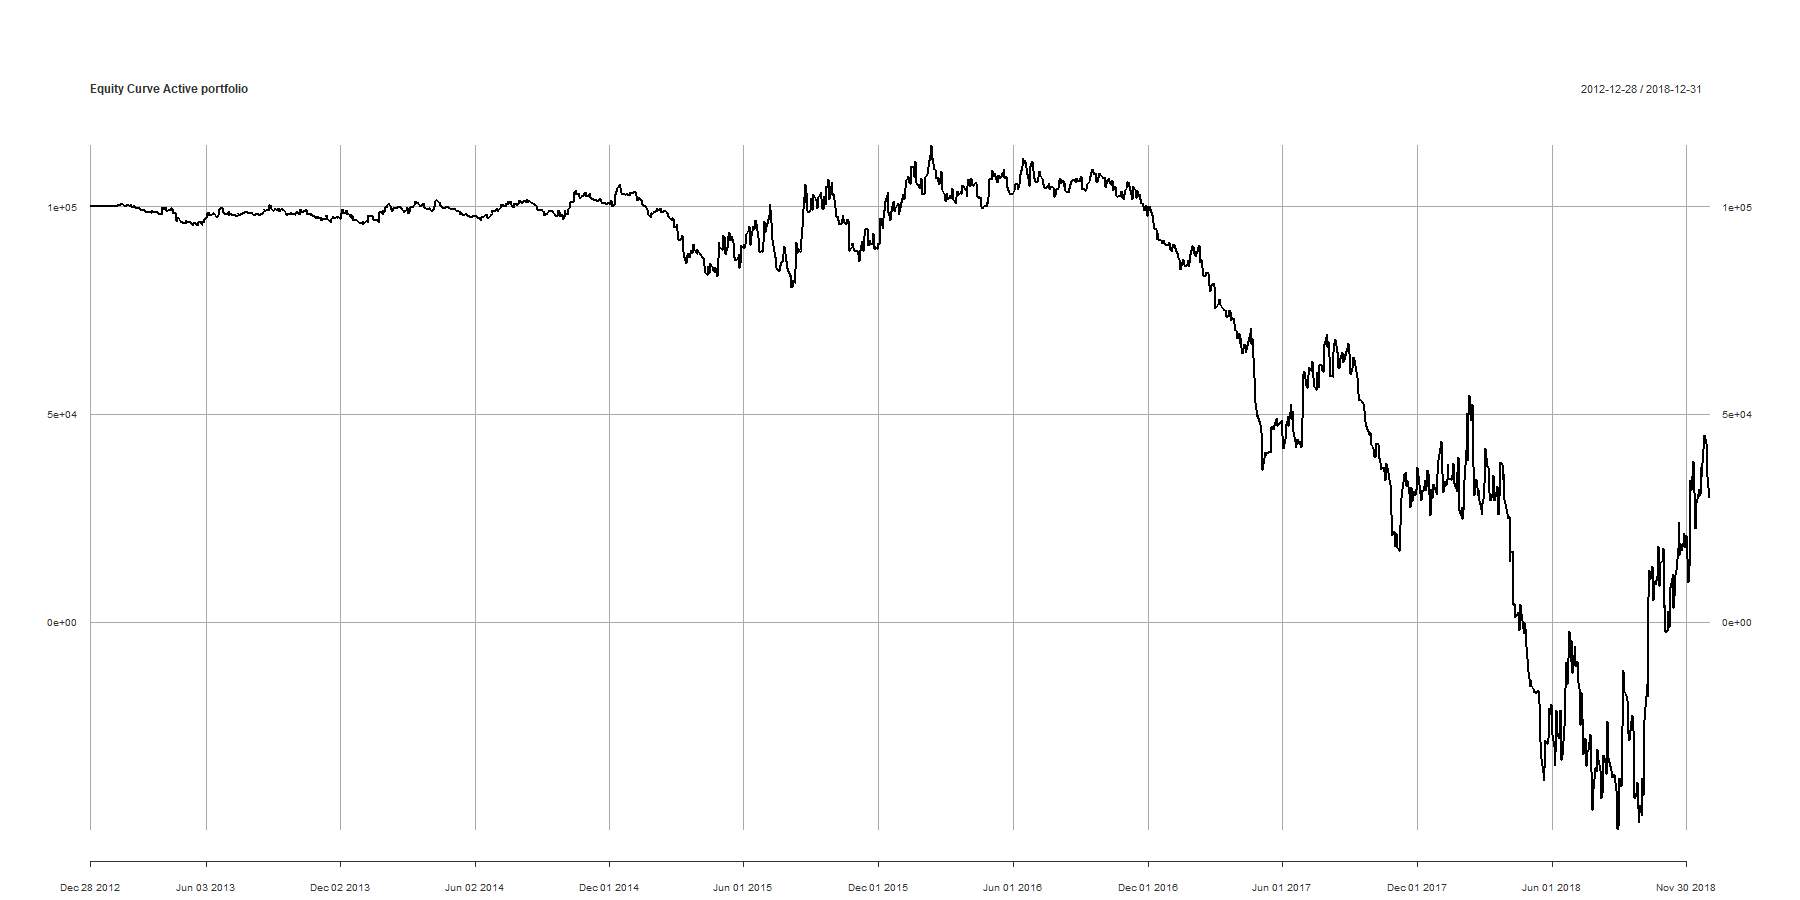
\includegraphics{"D:/2017-2018/data_analysis/technical_analysis/report/equity_active.png"}
\caption{Account Capital level evolution of active positions}
\end{figure}

\hypertarget{benchmarking-with-buy-and-hold-strategy}{%
\subsubsection{Benchmarking with buy-and-hold
strategy}\label{benchmarking-with-buy-and-hold-strategy}}

The negative performance of our active portfolio strategy prompts the
comparison with a passive strategy. We now implement a buy and hold
strategy, over the same timeframe as before, with the same stocks we
considered for our active strategy. Here we will allocate equal parts of
the initial capital to each of the five stocks, and execute a buy order
for each on the first day of observations. On the last day, we sell all
the stocks we had bought. Thus, the increase(reduction) in the stock
price will determine our gains(losses).

\begin{verbatim}
## [1] "Set capital to 100,000 Euros "
## [1] "2012-12-28 00:00:00 FP.PA 514 @ 38.91"
## [1] "2012-12-28 00:00:00 MC.PA 145 @ 137.800003"
## [1] "2012-12-28 00:00:00 SAN.PA 282 @ 70.730003"
## [1] "2012-12-28 00:00:00 AIR.PA 680 @ 29.395"
## [1] "2012-12-28 00:00:00 OR.PA 190 @ 104.800003"
## [1] "2018-12-31 00:00:00 FP.PA -514 @ 46.18"
## [1] "2018-12-31 00:00:00 MC.PA -145 @ 258.200012"
## [1] "2018-12-31 00:00:00 SAN.PA -282 @ 75.660004"
## [1] "2018-12-31 00:00:00 AIR.PA -680 @ 83.959999"
## [1] "2018-12-31 00:00:00 OR.PA -190 @ 201.199997"
\end{verbatim}

Since each stock price has risen during the five years examined, it can
be easily noted that this buy and hold strategy appears rather
profitable: our initial € 100.000 investment stake has increased by
about 80\%. At this stage, it is difficult to think that an active
strategy could have beaten the market. On the other hand, an in-depth
study is required to examine what factors determined such increases in
prices - whether it was that these five companies were particularly
successful, or perhaps the French economy was revamping after the
financial crisis. This in turn highlights the importance of an
appropriate market study that should accompany the creation of the
trading strategy. Clearly, investing is far from gambling, and coding or
mathemathical skills cannot make up for a poor understanding of the
markets and the economy.

\begin{figure}
\centering
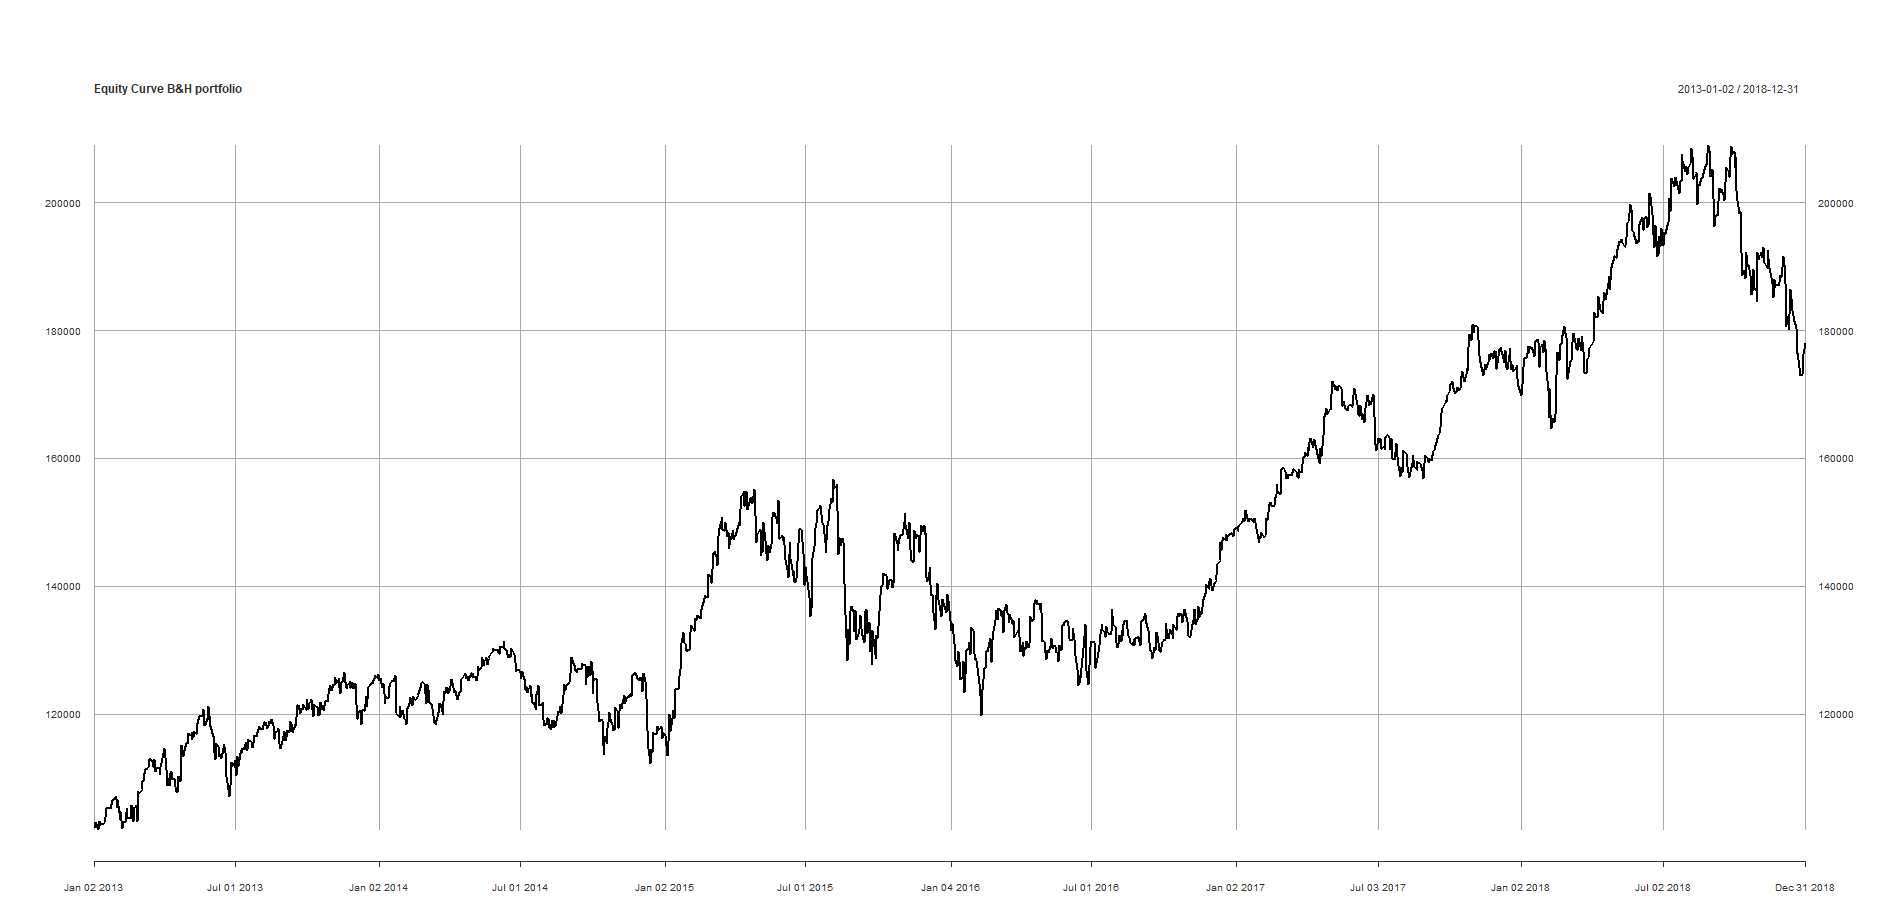
\includegraphics{"D:/2017-2018/data_analysis/technical_analysis/report/equity_BH.png"}
\caption{Account Capital level evolution of long positions in B\&H
strategy}
\end{figure}

\hypertarget{final-comments-and-future-steps}{%
\subsection{Final comments and future
steps}\label{final-comments-and-future-steps}}

It is clear that our strategy implementation lacks of several important
feautres, on which we already touched above. We left one important point
untackled - namely, the absence of a proper testing strategy. As Guy
Yollin illustrates \footnote{\url{http://www.r-programming.org/files}},
implementing a trading strategy would first require the so-called
\emph{walk-forward analysis}, which allows for a dynamic parametrization
of the model, with a lower impact of overfitting \footnote{\url{https://algotrading101.com/learn/what-is-walk-forward-optimization/}}.
Nevertheless, we would rather highlight the importance of having created
a realistic model, which can constitute a first, solid building block
towards a proper in-depth study of TA optimized applications to trading.

\newpage

\hypertarget{neural-networks}{%
\section{Neural networks}\label{neural-networks}}

Neural networks (NN) is a ``black box'' technique that finds non-linear
connections and recognize patterns between one or multiple inputs to
generate an output \footnote{\url{https://pathmind.com/wiki/neural-network}}
. We will test a 1-input NN \footnote{\url{http://rpubs.com/kapage/523169?fbclid=IwAR3RW_tVA_7SgCah7M0nmZL7anIL4gS_ZZ3dP_i_w8AOyQXoTMwXC_wQsoE}}
and a multiple-input NN \footnote{\url{https://www.analyticsvidhya.com/blog/2017/09/creating-visualizing-neural-network-in-r/?fbclid=IwAR0z9tD0-WFxG3zVs8YmFaLF7RGnszbizQrhyGdyZG1-GL-D5coqBOnTiZE}}
in the attempt to predict the next-day stock price of our 5 stocks, over
a period of 30 trading days, from the 16/11/2018 to the 31/12/2018.
Based on the predictions, we will develop an investing strategy where
everyday, for the above-mentioned 30 days, we will invest all our
capital (starting at 10,000 euro) into the stock that will have the
biggest predicted increase in price the next day, according to our
model. Consequently, the next day we will sell all our stocks bought the
previous day, and invest again all our capital with the same reasoning.
In this analysis, all commission and brokerage fees are ignored.

\hypertarget{benchmark}{%
\subsection{Benchmark}\label{benchmark}}

To evaluate the performance of the NN as an investment decision-maker,
instead of using a ROC Curve, we decided to compare it with a
diversified, long-term investment strategy, where the initial capital of
10.000 euro is invested equally in the 5 stocks (2.000 euro per stock)
at the beginning of the period (16/11/2018) and all stocks are then sold
at the end of the period (31/12/2018).

\begin{table}[H]

\caption{\label{tab:benchmark2}Benchmark strategy outcome}
\centering
\resizebox{\linewidth}{!}{
\begin{tabular}[t]{llllllll}
\toprule
Dates & AIR.PA & FP.PA & MC.PA & OR.PA & SAN.PA &   & Capital\\
\midrule
16/11/2018 & 95.86 & 92.88 & 45.19 & 65.09 & 77.09 & stock price(euro) & Total budget(euro)\\
 & 2000 & 2000 & 2000 & 2000 & 2000 & amount invested(euro) & 10000\\
 & 20.86 & 21.53 & 44.25 & 30.72 & 25.94 & N. of shares bought & \\
\hline
31/12/2018 & 98.59 & 83.95 & 39.47 & 61.5 & 72.01 & stock price(euro) & Total budget(euro)\\
 & 2056.89 & 1807.72 & 1746.87 & 1889.7 & 1868.22 & value in stocks(euro) & 9369.43\\
\bottomrule
\end{tabular}}
\end{table}

As can be seen, the benchmark strategy has a return of -6\%. Clearly,
the higher the return of the NN-based investments, the more successful
the NN algorithms will be. Moreover, in case of a return lower than -6\%
(lower than the ``naive'' strategy), the NN model will be considered as
not useful in predicting stock prices.

\hypertarget{input-nn}{%
\subsection{1-input NN}\label{input-nn}}

The first NN model is a single hidden layer neural network. In this
model there is one layer of input nodes that send weighted inputs to a
subsequent layer of receiving nodes. The \texttt{nnetar} function in the
forecast package fits a single hidden layer neural network model to a
timeseries. The function model approach is to use lagged values of the
time series as input data, reaching to a non-linear autoregressive
model. The model takes as input the stock prices starting from the
31/12/2016 to 31/12/2018. The goal is to predict the stock prices
between 16/11/2018 and 31/12/2018.

\begin{Shaded}
\begin{Highlighting}[]
\KeywordTok{library}\NormalTok{(prophet)}
\KeywordTok{library}\NormalTok{(quantmod)}
\KeywordTok{library}\NormalTok{(forecast)}
\KeywordTok{library}\NormalTok{(xlsx)}
\KeywordTok{library}\NormalTok{(tseries)}
\KeywordTok{library}\NormalTok{(timeSeries)}
\KeywordTok{library}\NormalTok{(dplyr)}
\KeywordTok{library}\NormalTok{(fGarch)}
\CommentTok{#Download the prices for the 5 stocks for the desired time frame}
\KeywordTok{getSymbols}\NormalTok{(}\StringTok{"AI.PA"}\NormalTok{, }\DataTypeTok{src=}\StringTok{"yahoo"}\NormalTok{, }\DataTypeTok{from=}\StringTok{"2016-12-31"}\NormalTok{, }\DataTypeTok{to=}\StringTok{"2018-12-31"}\NormalTok{)}
\KeywordTok{getSymbols}\NormalTok{(}\StringTok{"AIR.PA"}\NormalTok{, }\DataTypeTok{src=}\StringTok{"yahoo"}\NormalTok{, }\DataTypeTok{from=}\StringTok{"2016-12-31"}\NormalTok{, }\DataTypeTok{to=}\StringTok{"2018-12-31"}\NormalTok{)}
\KeywordTok{getSymbols}\NormalTok{(}\StringTok{"BN.PA"}\NormalTok{, }\DataTypeTok{src=}\StringTok{"yahoo"}\NormalTok{, }\DataTypeTok{from=}\StringTok{"2016-12-31"}\NormalTok{, }\DataTypeTok{to=}\StringTok{"2018-12-31"}\NormalTok{)}
\KeywordTok{getSymbols}\NormalTok{(}\StringTok{"BNP.PA"}\NormalTok{, }\DataTypeTok{src=}\StringTok{"yahoo"}\NormalTok{, }\DataTypeTok{from=}\StringTok{"2016-12-31"}\NormalTok{, }\DataTypeTok{to=}\StringTok{"2018-12-31"}\NormalTok{)}
\KeywordTok{getSymbols}\NormalTok{(}\StringTok{"DG.PA"}\NormalTok{, }\DataTypeTok{src=}\StringTok{"yahoo"}\NormalTok{, }\DataTypeTok{from=}\StringTok{"2016-12-31"}\NormalTok{, }\DataTypeTok{to=}\StringTok{"2018-12-31"}\NormalTok{)}

\NormalTok{alpha <-}\StringTok{ }\FloatTok{1.5}\OperatorTok{^}\NormalTok{(}\OperatorTok{-}\DecValTok{10}\NormalTok{)}
\end{Highlighting}
\end{Shaded}

We generate the predicted price of the 30 days for the 5 stocks with a
\texttt{for} loop, where the prices are predicted one at the time.
Although more computationally intense, in this way we are able to
predict the price of the day given all the ``information'' available
until the day before.

\begin{Shaded}
\begin{Highlighting}[]
\ControlFlowTok{for}\NormalTok{ (n }\ControlFlowTok{in} \DecValTok{1}\OperatorTok{:}\DecValTok{30}\NormalTok{)\{}
\NormalTok{  close_price <-}\StringTok{ }\KeywordTok{as.numeric}\NormalTok{(AIR.PA[}\DecValTok{1}\OperatorTok{:}\DecValTok{479}\OperatorTok{+}\NormalTok{n,}\StringTok{'AIR.PA.Close'}\NormalTok{])}
\CommentTok{#Hidden layers creation}
\NormalTok{  alpha <-}\StringTok{ }\FloatTok{1.5}\OperatorTok{^}\NormalTok{(}\OperatorTok{-}\DecValTok{10}\NormalTok{) }
\NormalTok{  hn <-}\StringTok{ }\KeywordTok{length}\NormalTok{(close_price)}\OperatorTok{/}\NormalTok{(alpha}\OperatorTok{*}\NormalTok{(}\KeywordTok{length}\NormalTok{(close_price)}\OperatorTok{+}\DecValTok{1}\NormalTok{))}
\CommentTok{#Fitting nnetar}
\NormalTok{  lambda <-}\StringTok{ }\KeywordTok{BoxCox.lambda}\NormalTok{(close_price)}
\NormalTok{  dnn_pred <-}\StringTok{ }\KeywordTok{nnetar}\NormalTok{(close_price, }\DataTypeTok{size=}\NormalTok{ hn, }\DataTypeTok{lambda =}\NormalTok{ lambda) }
\NormalTok{  dnn_forecast <-}\StringTok{ }\KeywordTok{forecast}\NormalTok{(dnn_pred, }\DataTypeTok{h=} \DecValTok{1}\NormalTok{, }\DataTypeTok{PI =} \OtherTok{TRUE}\NormalTok{)   }
\NormalTok{  AIR.PA.P[n] =}\StringTok{ }\NormalTok{dnn_forecast[[}\StringTok{"mean"}\NormalTok{]] }
\NormalTok{\}}

\ControlFlowTok{for}\NormalTok{ (n }\ControlFlowTok{in} \DecValTok{1}\OperatorTok{:}\DecValTok{30}\NormalTok{)\{}
\NormalTok{   close_price <-}\StringTok{ }\KeywordTok{as.numeric}\NormalTok{(BN.PA[}\DecValTok{1}\OperatorTok{:}\DecValTok{479}\OperatorTok{+}\NormalTok{n,}\StringTok{'BN.PA.Close'}\NormalTok{])}
\NormalTok{   hn <-}\StringTok{ }\KeywordTok{length}\NormalTok{(close_price)}\OperatorTok{/}\NormalTok{(alpha}\OperatorTok{*}\NormalTok{(}\KeywordTok{length}\NormalTok{(close_price)}\OperatorTok{+}\DecValTok{1}\NormalTok{))}
\NormalTok{   lambda <-}\StringTok{ }\KeywordTok{BoxCox.lambda}\NormalTok{(close_price)}
\NormalTok{   dnn_pred <-}\StringTok{ }\KeywordTok{nnetar}\NormalTok{(close_price, }\DataTypeTok{size=}\NormalTok{ hn, }\DataTypeTok{lambda =}\NormalTok{ lambda)}
\NormalTok{   dnn_forecast <-}\StringTok{ }\KeywordTok{forecast}\NormalTok{(dnn_pred, }\DataTypeTok{h=} \DecValTok{1}\NormalTok{, }\DataTypeTok{PI =} \OtherTok{TRUE}\NormalTok{)}
\NormalTok{   BN.PA.P[n] =}\StringTok{ }\NormalTok{dnn_forecast[[}\StringTok{"mean"}\NormalTok{]]}
\NormalTok{ \}}
 
 \CommentTok{#We run the same for loop above also for AI.PA, BNP.PA and DG.PA}
\end{Highlighting}
\end{Shaded}

We create a table with the predicted daily increase in price for every
stock during the 30 days. After that, we will identify the stock with
the highest predicted increase in price for every day. This will be the
stock where to invest all the capital for the day.

\begin{Shaded}
\begin{Highlighting}[]
\NormalTok{AIR.LOL <-}\StringTok{ }\NormalTok{AIR.PA.P }\OperatorTok{-}\StringTok{ }\KeywordTok{as.numeric}\NormalTok{(AIR.PA[}\DecValTok{480}\OperatorTok{:}\DecValTok{509}\NormalTok{,}\StringTok{'AIR.PA.Close'}\NormalTok{])}
\NormalTok{BN.LOL <-}\StringTok{ }\NormalTok{BN.PA.P }\OperatorTok{-}\StringTok{ }\KeywordTok{as.numeric}\NormalTok{(BN.PA[}\DecValTok{480}\OperatorTok{:}\DecValTok{509}\NormalTok{,}\StringTok{'BN.PA.Close'}\NormalTok{])}
\NormalTok{BNP.LOL <-}\StringTok{ }\NormalTok{BNP.PA.P }\OperatorTok{-}\StringTok{ }\KeywordTok{as.numeric}\NormalTok{(BNP.PA[}\DecValTok{480}\OperatorTok{:}\DecValTok{509}\NormalTok{,}\StringTok{'BNP.PA.Close'}\NormalTok{])}
\NormalTok{DG.LOL <-}\StringTok{ }\NormalTok{DG.PA.P }\OperatorTok{-}\StringTok{ }\KeywordTok{as.numeric}\NormalTok{(DG.PA[}\DecValTok{480}\OperatorTok{:}\DecValTok{509}\NormalTok{,}\StringTok{'DG.PA.Close'}\NormalTok{])}

\NormalTok{df =}\StringTok{ }\KeywordTok{data.frame}\NormalTok{(AI.LOL,AIR.LOL,BN.LOL,BNP.LOL,DG.LOL)}

\ControlFlowTok{for}\NormalTok{ (n }\ControlFlowTok{in} \DecValTok{1}\OperatorTok{:}\DecValTok{30}\NormalTok{)\{}
   \ControlFlowTok{if}\NormalTok{ (}\KeywordTok{max}\NormalTok{(df[n,]) }\OperatorTok{==}\StringTok{ }\NormalTok{df[n,}\StringTok{"AI.LOL"}\NormalTok{])\{}
\NormalTok{   AI.DIF[n] =}\StringTok{ "AI.PA"}
\NormalTok{   \} }\ControlFlowTok{else} \ControlFlowTok{if}\NormalTok{ (}\KeywordTok{max}\NormalTok{(df[n,]) }\OperatorTok{==}\StringTok{ }\NormalTok{df[n,}\StringTok{"AIR.LOL"}\NormalTok{])\{}
\NormalTok{   AI.DIF[n] =}\StringTok{ "AIR.PA"}
\NormalTok{   \} }\ControlFlowTok{else} \ControlFlowTok{if}\NormalTok{ (}\KeywordTok{max}\NormalTok{(df[n,]) }\OperatorTok{==}\StringTok{ }\NormalTok{df[n,}\StringTok{"BN.LOL"}\NormalTok{])\{}
\NormalTok{   AI.DIF[n] =}\StringTok{ "BN.PA"}
\NormalTok{   \} }\ControlFlowTok{else} \ControlFlowTok{if}\NormalTok{ (}\KeywordTok{max}\NormalTok{(df[n,]) }\OperatorTok{==}\StringTok{ }\NormalTok{df[n,}\StringTok{"BNP.LOL"}\NormalTok{])\{}
\NormalTok{   AI.DIF[n] =}\StringTok{ "BNP.PA"}
\NormalTok{   \} }\ControlFlowTok{else} \ControlFlowTok{if}\NormalTok{ (}\KeywordTok{max}\NormalTok{(df[n,]) }\OperatorTok{==}\StringTok{ }\NormalTok{df[n,}\StringTok{"DG.LOL"}\NormalTok{])\{}
\NormalTok{   AI.DIF[n] =}\StringTok{ "DG.PA"}
\NormalTok{   \}}
\NormalTok{\}}
\end{Highlighting}
\end{Shaded}

\begin{longtable}[]{@{}llllllllll@{}}
\caption{1-input NN strategy outcome}\tabularnewline
\toprule
\begin{minipage}[b]{0.05\columnwidth}\raggedright
Day\strut
\end{minipage} & \begin{minipage}[b]{0.07\columnwidth}\raggedright
Invest in\strut
\end{minipage} & \begin{minipage}[b]{0.11\columnwidth}\raggedright
date\strut
\end{minipage} & \begin{minipage}[b]{0.07\columnwidth}\raggedright
AI\strut
\end{minipage} & \begin{minipage}[b]{0.07\columnwidth}\raggedright
AIR\strut
\end{minipage} & \begin{minipage}[b]{0.07\columnwidth}\raggedright
BNP\strut
\end{minipage} & \begin{minipage}[b]{0.07\columnwidth}\raggedright
BN\strut
\end{minipage} & \begin{minipage}[b]{0.07\columnwidth}\raggedright
DG\strut
\end{minipage} & \begin{minipage}[b]{0.08\columnwidth}\raggedright
\#shares bought\strut
\end{minipage} & \begin{minipage}[b]{0.09\columnwidth}\raggedright
€ Value\strut
\end{minipage}\tabularnewline
\midrule
\endfirsthead
\toprule
\begin{minipage}[b]{0.05\columnwidth}\raggedright
Day\strut
\end{minipage} & \begin{minipage}[b]{0.07\columnwidth}\raggedright
Invest in\strut
\end{minipage} & \begin{minipage}[b]{0.11\columnwidth}\raggedright
date\strut
\end{minipage} & \begin{minipage}[b]{0.07\columnwidth}\raggedright
AI\strut
\end{minipage} & \begin{minipage}[b]{0.07\columnwidth}\raggedright
AIR\strut
\end{minipage} & \begin{minipage}[b]{0.07\columnwidth}\raggedright
BNP\strut
\end{minipage} & \begin{minipage}[b]{0.07\columnwidth}\raggedright
BN\strut
\end{minipage} & \begin{minipage}[b]{0.07\columnwidth}\raggedright
DG\strut
\end{minipage} & \begin{minipage}[b]{0.08\columnwidth}\raggedright
\#shares bought\strut
\end{minipage} & \begin{minipage}[b]{0.09\columnwidth}\raggedright
€ Value\strut
\end{minipage}\tabularnewline
\midrule
\endhead
\begin{minipage}[t]{0.05\columnwidth}\raggedright
1\strut
\end{minipage} & \begin{minipage}[t]{0.07\columnwidth}\raggedright
BNP\strut
\end{minipage} & \begin{minipage}[t]{0.11\columnwidth}\raggedright
16/11/2018\strut
\end{minipage} & \begin{minipage}[t]{0.07\columnwidth}\raggedright
95.86\strut
\end{minipage} & \begin{minipage}[t]{0.07\columnwidth}\raggedright
92.88\strut
\end{minipage} & \begin{minipage}[t]{0.07\columnwidth}\raggedright
45.19\strut
\end{minipage} & \begin{minipage}[t]{0.07\columnwidth}\raggedright
65.09\strut
\end{minipage} & \begin{minipage}[t]{0.07\columnwidth}\raggedright
77.09\strut
\end{minipage} & \begin{minipage}[t]{0.08\columnwidth}\raggedright
221.26\strut
\end{minipage} & \begin{minipage}[t]{0.09\columnwidth}\raggedright
10000\strut
\end{minipage}\tabularnewline
\begin{minipage}[t]{0.05\columnwidth}\raggedright
2\strut
\end{minipage} & \begin{minipage}[t]{0.07\columnwidth}\raggedright
BNP\strut
\end{minipage} & \begin{minipage}[t]{0.11\columnwidth}\raggedright
19/11/2018\strut
\end{minipage} & \begin{minipage}[t]{0.07\columnwidth}\raggedright
95.40\strut
\end{minipage} & \begin{minipage}[t]{0.07\columnwidth}\raggedright
92.57\strut
\end{minipage} & \begin{minipage}[t]{0.07\columnwidth}\raggedright
45.28\strut
\end{minipage} & \begin{minipage}[t]{0.07\columnwidth}\raggedright
64.70\strut
\end{minipage} & \begin{minipage}[t]{0.07\columnwidth}\raggedright
76.80\strut
\end{minipage} & \begin{minipage}[t]{0.08\columnwidth}\raggedright
221.26\strut
\end{minipage} & \begin{minipage}[t]{0.09\columnwidth}\raggedright
10019.91\strut
\end{minipage}\tabularnewline
\begin{minipage}[t]{0.05\columnwidth}\raggedright
3\strut
\end{minipage} & \begin{minipage}[t]{0.07\columnwidth}\raggedright
BNP\strut
\end{minipage} & \begin{minipage}[t]{0.11\columnwidth}\raggedright
20/11/2018\strut
\end{minipage} & \begin{minipage}[t]{0.07\columnwidth}\raggedright
93.5\strut
\end{minipage} & \begin{minipage}[t]{0.07\columnwidth}\raggedright
91.07\strut
\end{minipage} & \begin{minipage}[t]{0.07\columnwidth}\raggedright
44.30\strut
\end{minipage} & \begin{minipage}[t]{0.07\columnwidth}\raggedright
64.98\strut
\end{minipage} & \begin{minipage}[t]{0.07\columnwidth}\raggedright
76.37\strut
\end{minipage} & \begin{minipage}[t]{0.08\columnwidth}\raggedright
221.26\strut
\end{minipage} & \begin{minipage}[t]{0.09\columnwidth}\raggedright
9803.07\strut
\end{minipage}\tabularnewline
\begin{minipage}[t]{0.05\columnwidth}\raggedright
4\strut
\end{minipage} & \begin{minipage}[t]{0.07\columnwidth}\raggedright
AI\strut
\end{minipage} & \begin{minipage}[t]{0.11\columnwidth}\raggedright
21/11/2018\strut
\end{minipage} & \begin{minipage}[t]{0.07\columnwidth}\raggedright
94.22\strut
\end{minipage} & \begin{minipage}[t]{0.07\columnwidth}\raggedright
93.16\strut
\end{minipage} & \begin{minipage}[t]{0.07\columnwidth}\raggedright
44.79\strut
\end{minipage} & \begin{minipage}[t]{0.07\columnwidth}\raggedright
65.41\strut
\end{minipage} & \begin{minipage}[t]{0.07\columnwidth}\raggedright
77.01\strut
\end{minipage} & \begin{minipage}[t]{0.08\columnwidth}\raggedright
105.17\strut
\end{minipage} & \begin{minipage}[t]{0.09\columnwidth}\raggedright
9910.38\strut
\end{minipage}\tabularnewline
\begin{minipage}[t]{0.05\columnwidth}\raggedright
5\strut
\end{minipage} & \begin{minipage}[t]{0.07\columnwidth}\raggedright
AIR\strut
\end{minipage} & \begin{minipage}[t]{0.11\columnwidth}\raggedright
22/11/2018\strut
\end{minipage} & \begin{minipage}[t]{0.07\columnwidth}\raggedright
93.31\strut
\end{minipage} & \begin{minipage}[t]{0.07\columnwidth}\raggedright
92.33\strut
\end{minipage} & \begin{minipage}[t]{0.07\columnwidth}\raggedright
44.28\strut
\end{minipage} & \begin{minipage}[t]{0.07\columnwidth}\raggedright
65.27\strut
\end{minipage} & \begin{minipage}[t]{0.07\columnwidth}\raggedright
76.62\strut
\end{minipage} & \begin{minipage}[t]{0.08\columnwidth}\raggedright
106.30\strut
\end{minipage} & \begin{minipage}[t]{0.09\columnwidth}\raggedright
9814.77\strut
\end{minipage}\tabularnewline
\begin{minipage}[t]{0.05\columnwidth}\raggedright
6\strut
\end{minipage} & \begin{minipage}[t]{0.07\columnwidth}\raggedright
AI\strut
\end{minipage} & \begin{minipage}[t]{0.11\columnwidth}\raggedright
23/11/2018\strut
\end{minipage} & \begin{minipage}[t]{0.07\columnwidth}\raggedright
93.86\strut
\end{minipage} & \begin{minipage}[t]{0.07\columnwidth}\raggedright
93.41\strut
\end{minipage} & \begin{minipage}[t]{0.07\columnwidth}\raggedright
44.36\strut
\end{minipage} & \begin{minipage}[t]{0.07\columnwidth}\raggedright
65.87\strut
\end{minipage} & \begin{minipage}[t]{0.07\columnwidth}\raggedright
76.86\strut
\end{minipage} & \begin{minipage}[t]{0.08\columnwidth}\raggedright
105.78\strut
\end{minipage} & \begin{minipage}[t]{0.09\columnwidth}\raggedright
9929.57\strut
\end{minipage}\tabularnewline
\begin{minipage}[t]{0.05\columnwidth}\raggedright
7\strut
\end{minipage} & \begin{minipage}[t]{0.07\columnwidth}\raggedright
AI\strut
\end{minipage} & \begin{minipage}[t]{0.11\columnwidth}\raggedright
26/11/2018\strut
\end{minipage} & \begin{minipage}[t]{0.07\columnwidth}\raggedright
95.86\strut
\end{minipage} & \begin{minipage}[t]{0.07\columnwidth}\raggedright
93.58\strut
\end{minipage} & \begin{minipage}[t]{0.07\columnwidth}\raggedright
45.34\strut
\end{minipage} & \begin{minipage}[t]{0.07\columnwidth}\raggedright
65.82\strut
\end{minipage} & \begin{minipage}[t]{0.07\columnwidth}\raggedright
78.54\strut
\end{minipage} & \begin{minipage}[t]{0.08\columnwidth}\raggedright
105.78\strut
\end{minipage} & \begin{minipage}[t]{0.09\columnwidth}\raggedright
10141.15\strut
\end{minipage}\tabularnewline
\begin{minipage}[t]{0.05\columnwidth}\raggedright
8\strut
\end{minipage} & \begin{minipage}[t]{0.07\columnwidth}\raggedright
AIR\strut
\end{minipage} & \begin{minipage}[t]{0.11\columnwidth}\raggedright
27/11/2018\strut
\end{minipage} & \begin{minipage}[t]{0.07\columnwidth}\raggedright
94.86\strut
\end{minipage} & \begin{minipage}[t]{0.07\columnwidth}\raggedright
93.69\strut
\end{minipage} & \begin{minipage}[t]{0.07\columnwidth}\raggedright
45.08\strut
\end{minipage} & \begin{minipage}[t]{0.07\columnwidth}\raggedright
66.41\strut
\end{minipage} & \begin{minipage}[t]{0.07\columnwidth}\raggedright
78.16\strut
\end{minipage} & \begin{minipage}[t]{0.08\columnwidth}\raggedright
107.10\strut
\end{minipage} & \begin{minipage}[t]{0.09\columnwidth}\raggedright
10035.36\strut
\end{minipage}\tabularnewline
\begin{minipage}[t]{0.05\columnwidth}\raggedright
9\strut
\end{minipage} & \begin{minipage}[t]{0.07\columnwidth}\raggedright
BNP\strut
\end{minipage} & \begin{minipage}[t]{0.11\columnwidth}\raggedright
28/11/2018\strut
\end{minipage} & \begin{minipage}[t]{0.07\columnwidth}\raggedright
94.36\strut
\end{minipage} & \begin{minipage}[t]{0.07\columnwidth}\raggedright
93.5\strut
\end{minipage} & \begin{minipage}[t]{0.07\columnwidth}\raggedright
44.75\strut
\end{minipage} & \begin{minipage}[t]{0.07\columnwidth}\raggedright
65.41\strut
\end{minipage} & \begin{minipage}[t]{0.07\columnwidth}\raggedright
77.95\strut
\end{minipage} & \begin{minipage}[t]{0.08\columnwidth}\raggedright
223.75\strut
\end{minipage} & \begin{minipage}[t]{0.09\columnwidth}\raggedright
10013.94\strut
\end{minipage}\tabularnewline
\begin{minipage}[t]{0.05\columnwidth}\raggedright
10\strut
\end{minipage} & \begin{minipage}[t]{0.07\columnwidth}\raggedright
AI\strut
\end{minipage} & \begin{minipage}[t]{0.11\columnwidth}\raggedright
29/11/2018\strut
\end{minipage} & \begin{minipage}[t]{0.07\columnwidth}\raggedright
94.68\strut
\end{minipage} & \begin{minipage}[t]{0.07\columnwidth}\raggedright
94.86\strut
\end{minipage} & \begin{minipage}[t]{0.07\columnwidth}\raggedright
44.77\strut
\end{minipage} & \begin{minipage}[t]{0.07\columnwidth}\raggedright
65.54\strut
\end{minipage} & \begin{minipage}[t]{0.07\columnwidth}\raggedright
77.58\strut
\end{minipage} & \begin{minipage}[t]{0.08\columnwidth}\raggedright
105.81\strut
\end{minipage} & \begin{minipage}[t]{0.09\columnwidth}\raggedright
10018.42\strut
\end{minipage}\tabularnewline
\begin{minipage}[t]{0.05\columnwidth}\raggedright
11\strut
\end{minipage} & \begin{minipage}[t]{0.07\columnwidth}\raggedright
AI\strut
\end{minipage} & \begin{minipage}[t]{0.11\columnwidth}\raggedright
30/11/2018\strut
\end{minipage} & \begin{minipage}[t]{0.07\columnwidth}\raggedright
97.04\strut
\end{minipage} & \begin{minipage}[t]{0.07\columnwidth}\raggedright
94.62\strut
\end{minipage} & \begin{minipage}[t]{0.07\columnwidth}\raggedright
44.37\strut
\end{minipage} & \begin{minipage}[t]{0.07\columnwidth}\raggedright
66.05\strut
\end{minipage} & \begin{minipage}[t]{0.07\columnwidth}\raggedright
77.09\strut
\end{minipage} & \begin{minipage}[t]{0.08\columnwidth}\raggedright
105.81\strut
\end{minipage} & \begin{minipage}[t]{0.09\columnwidth}\raggedright
10268.51\strut
\end{minipage}\tabularnewline
\begin{minipage}[t]{0.05\columnwidth}\raggedright
12\strut
\end{minipage} & \begin{minipage}[t]{0.07\columnwidth}\raggedright
AI\strut
\end{minipage} & \begin{minipage}[t]{0.11\columnwidth}\raggedright
03/12/2018\strut
\end{minipage} & \begin{minipage}[t]{0.07\columnwidth}\raggedright
97.27\strut
\end{minipage} & \begin{minipage}[t]{0.07\columnwidth}\raggedright
95.69\strut
\end{minipage} & \begin{minipage}[t]{0.07\columnwidth}\raggedright
44.84\strut
\end{minipage} & \begin{minipage}[t]{0.07\columnwidth}\raggedright
65.41\strut
\end{minipage} & \begin{minipage}[t]{0.07\columnwidth}\raggedright
75.40\strut
\end{minipage} & \begin{minipage}[t]{0.08\columnwidth}\raggedright
105.81\strut
\end{minipage} & \begin{minipage}[t]{0.09\columnwidth}\raggedright
10292.56\strut
\end{minipage}\tabularnewline
\begin{minipage}[t]{0.05\columnwidth}\raggedright
13\strut
\end{minipage} & \begin{minipage}[t]{0.07\columnwidth}\raggedright
AI\strut
\end{minipage} & \begin{minipage}[t]{0.11\columnwidth}\raggedright
04/12/2018\strut
\end{minipage} & \begin{minipage}[t]{0.07\columnwidth}\raggedright
97.45\strut
\end{minipage} & \begin{minipage}[t]{0.07\columnwidth}\raggedright
94.26\strut
\end{minipage} & \begin{minipage}[t]{0.07\columnwidth}\raggedright
43.86\strut
\end{minipage} & \begin{minipage}[t]{0.07\columnwidth}\raggedright
65.52\strut
\end{minipage} & \begin{minipage}[t]{0.07\columnwidth}\raggedright
76.66\strut
\end{minipage} & \begin{minipage}[t]{0.08\columnwidth}\raggedright
105.81\strut
\end{minipage} & \begin{minipage}[t]{0.09\columnwidth}\raggedright
10311.81\strut
\end{minipage}\tabularnewline
\begin{minipage}[t]{0.05\columnwidth}\raggedright
14\strut
\end{minipage} & \begin{minipage}[t]{0.07\columnwidth}\raggedright
BNP\strut
\end{minipage} & \begin{minipage}[t]{0.11\columnwidth}\raggedright
05/12/2018\strut
\end{minipage} & \begin{minipage}[t]{0.07\columnwidth}\raggedright
96.45\strut
\end{minipage} & \begin{minipage}[t]{0.07\columnwidth}\raggedright
92.30\strut
\end{minipage} & \begin{minipage}[t]{0.07\columnwidth}\raggedright
43.41\strut
\end{minipage} & \begin{minipage}[t]{0.07\columnwidth}\raggedright
64.58\strut
\end{minipage} & \begin{minipage}[t]{0.07\columnwidth}\raggedright
74.66\strut
\end{minipage} & \begin{minipage}[t]{0.08\columnwidth}\raggedright
235.05\strut
\end{minipage} & \begin{minipage}[t]{0.09\columnwidth}\raggedright
10206.00\strut
\end{minipage}\tabularnewline
\begin{minipage}[t]{0.05\columnwidth}\raggedright
15\strut
\end{minipage} & \begin{minipage}[t]{0.07\columnwidth}\raggedright
DG\strut
\end{minipage} & \begin{minipage}[t]{0.11\columnwidth}\raggedright
06/12/2018\strut
\end{minipage} & \begin{minipage}[t]{0.07\columnwidth}\raggedright
94.63\strut
\end{minipage} & \begin{minipage}[t]{0.07\columnwidth}\raggedright
88.63\strut
\end{minipage} & \begin{minipage}[t]{0.07\columnwidth}\raggedright
41.78\strut
\end{minipage} & \begin{minipage}[t]{0.07\columnwidth}\raggedright
63.43\strut
\end{minipage} & \begin{minipage}[t]{0.07\columnwidth}\raggedright
70.98\strut
\end{minipage} & \begin{minipage}[t]{0.08\columnwidth}\raggedright
138.37\strut
\end{minipage} & \begin{minipage}[t]{0.09\columnwidth}\raggedright
9821.69\strut
\end{minipage}\tabularnewline
\begin{minipage}[t]{0.05\columnwidth}\raggedright
16\strut
\end{minipage} & \begin{minipage}[t]{0.07\columnwidth}\raggedright
AI\strut
\end{minipage} & \begin{minipage}[t]{0.11\columnwidth}\raggedright
07/12/2018\strut
\end{minipage} & \begin{minipage}[t]{0.07\columnwidth}\raggedright
95.86\strut
\end{minipage} & \begin{minipage}[t]{0.07\columnwidth}\raggedright
89.07\strut
\end{minipage} & \begin{minipage}[t]{0.07\columnwidth}\raggedright
41.59\strut
\end{minipage} & \begin{minipage}[t]{0.07\columnwidth}\raggedright
63.79\strut
\end{minipage} & \begin{minipage}[t]{0.07\columnwidth}\raggedright
72.68\strut
\end{minipage} & \begin{minipage}[t]{0.08\columnwidth}\raggedright
104.90\strut
\end{minipage} & \begin{minipage}[t]{0.09\columnwidth}\raggedright
10056.92\strut
\end{minipage}\tabularnewline
\begin{minipage}[t]{0.05\columnwidth}\raggedright
17\strut
\end{minipage} & \begin{minipage}[t]{0.07\columnwidth}\raggedright
DG\strut
\end{minipage} & \begin{minipage}[t]{0.11\columnwidth}\raggedright
10/12/2018\strut
\end{minipage} & \begin{minipage}[t]{0.07\columnwidth}\raggedright
95.77\strut
\end{minipage} & \begin{minipage}[t]{0.07\columnwidth}\raggedright
87.48\strut
\end{minipage} & \begin{minipage}[t]{0.07\columnwidth}\raggedright
40.40\strut
\end{minipage} & \begin{minipage}[t]{0.07\columnwidth}\raggedright
62.97\strut
\end{minipage} & \begin{minipage}[t]{0.07\columnwidth}\raggedright
71.66\strut
\end{minipage} & \begin{minipage}[t]{0.08\columnwidth}\raggedright
140.20\strut
\end{minipage} & \begin{minipage}[t]{0.09\columnwidth}\raggedright
10047.38\strut
\end{minipage}\tabularnewline
\begin{minipage}[t]{0.05\columnwidth}\raggedright
18\strut
\end{minipage} & \begin{minipage}[t]{0.07\columnwidth}\raggedright
DG\strut
\end{minipage} & \begin{minipage}[t]{0.11\columnwidth}\raggedright
11/12/2018\strut
\end{minipage} & \begin{minipage}[t]{0.07\columnwidth}\raggedright
96.45\strut
\end{minipage} & \begin{minipage}[t]{0.07\columnwidth}\raggedright
88.59\strut
\end{minipage} & \begin{minipage}[t]{0.07\columnwidth}\raggedright
40.68\strut
\end{minipage} & \begin{minipage}[t]{0.07\columnwidth}\raggedright
62.81\strut
\end{minipage} & \begin{minipage}[t]{0.07\columnwidth}\raggedright
73.69\strut
\end{minipage} & \begin{minipage}[t]{0.08\columnwidth}\raggedright
140.20\strut
\end{minipage} & \begin{minipage}[t]{0.09\columnwidth}\raggedright
10333.41\strut
\end{minipage}\tabularnewline
\begin{minipage}[t]{0.05\columnwidth}\raggedright
19\strut
\end{minipage} & \begin{minipage}[t]{0.07\columnwidth}\raggedright
AI\strut
\end{minipage} & \begin{minipage}[t]{0.11\columnwidth}\raggedright
12/12/2018\strut
\end{minipage} & \begin{minipage}[t]{0.07\columnwidth}\raggedright
97.54\strut
\end{minipage} & \begin{minipage}[t]{0.07\columnwidth}\raggedright
91.48\strut
\end{minipage} & \begin{minipage}[t]{0.07\columnwidth}\raggedright
41.90\strut
\end{minipage} & \begin{minipage}[t]{0.07\columnwidth}\raggedright
64.12\strut
\end{minipage} & \begin{minipage}[t]{0.07\columnwidth}\raggedright
74.77\strut
\end{minipage} & \begin{minipage}[t]{0.08\columnwidth}\raggedright
107.48\strut
\end{minipage} & \begin{minipage}[t]{0.09\columnwidth}\raggedright
10484.84\strut
\end{minipage}\tabularnewline
\begin{minipage}[t]{0.05\columnwidth}\raggedright
20\strut
\end{minipage} & \begin{minipage}[t]{0.07\columnwidth}\raggedright
BN\strut
\end{minipage} & \begin{minipage}[t]{0.11\columnwidth}\raggedright
13/12/2018\strut
\end{minipage} & \begin{minipage}[t]{0.07\columnwidth}\raggedright
97.63\strut
\end{minipage} & \begin{minipage}[t]{0.07\columnwidth}\raggedright
89.97\strut
\end{minipage} & \begin{minipage}[t]{0.07\columnwidth}\raggedright
42.18\strut
\end{minipage} & \begin{minipage}[t]{0.07\columnwidth}\raggedright
64.32\strut
\end{minipage} & \begin{minipage}[t]{0.07\columnwidth}\raggedright
74.5\strut
\end{minipage} & \begin{minipage}[t]{0.08\columnwidth}\raggedright
163.16\strut
\end{minipage} & \begin{minipage}[t]{0.09\columnwidth}\raggedright
10494.62\strut
\end{minipage}\tabularnewline
\begin{minipage}[t]{0.05\columnwidth}\raggedright
21\strut
\end{minipage} & \begin{minipage}[t]{0.07\columnwidth}\raggedright
BNP\strut
\end{minipage} & \begin{minipage}[t]{0.11\columnwidth}\raggedright
14/12/2018\strut
\end{minipage} & \begin{minipage}[t]{0.07\columnwidth}\raggedright
97.45\strut
\end{minipage} & \begin{minipage}[t]{0.07\columnwidth}\raggedright
88.66\strut
\end{minipage} & \begin{minipage}[t]{0.07\columnwidth}\raggedright
41.59\strut
\end{minipage} & \begin{minipage}[t]{0.07\columnwidth}\raggedright
64.08\strut
\end{minipage} & \begin{minipage}[t]{0.07\columnwidth}\raggedright
73.51\strut
\end{minipage} & \begin{minipage}[t]{0.08\columnwidth}\raggedright
251.36\strut
\end{minipage} & \begin{minipage}[t]{0.09\columnwidth}\raggedright
10455.46\strut
\end{minipage}\tabularnewline
\begin{minipage}[t]{0.05\columnwidth}\raggedright
22\strut
\end{minipage} & \begin{minipage}[t]{0.07\columnwidth}\raggedright
DG\strut
\end{minipage} & \begin{minipage}[t]{0.11\columnwidth}\raggedright
17/12/2018\strut
\end{minipage} & \begin{minipage}[t]{0.07\columnwidth}\raggedright
96.68\strut
\end{minipage} & \begin{minipage}[t]{0.07\columnwidth}\raggedright
87.65\strut
\end{minipage} & \begin{minipage}[t]{0.07\columnwidth}\raggedright
40.58\strut
\end{minipage} & \begin{minipage}[t]{0.07\columnwidth}\raggedright
63.23\strut
\end{minipage} & \begin{minipage}[t]{0.07\columnwidth}\raggedright
72.36\strut
\end{minipage} & \begin{minipage}[t]{0.08\columnwidth}\raggedright
140.96\strut
\end{minipage} & \begin{minipage}[t]{0.09\columnwidth}\raggedright
10200.32\strut
\end{minipage}\tabularnewline
\begin{minipage}[t]{0.05\columnwidth}\raggedright
23\strut
\end{minipage} & \begin{minipage}[t]{0.07\columnwidth}\raggedright
DG\strut
\end{minipage} & \begin{minipage}[t]{0.11\columnwidth}\raggedright
18/12/2018\strut
\end{minipage} & \begin{minipage}[t]{0.07\columnwidth}\raggedright
95.68\strut
\end{minipage} & \begin{minipage}[t]{0.07\columnwidth}\raggedright
88.65\strut
\end{minipage} & \begin{minipage}[t]{0.07\columnwidth}\raggedright
40.55\strut
\end{minipage} & \begin{minipage}[t]{0.07\columnwidth}\raggedright
62.68\strut
\end{minipage} & \begin{minipage}[t]{0.07\columnwidth}\raggedright
71.33\strut
\end{minipage} & \begin{minipage}[t]{0.08\columnwidth}\raggedright
140.96\strut
\end{minipage} & \begin{minipage}[t]{0.09\columnwidth}\raggedright
10056.54\strut
\end{minipage}\tabularnewline
\begin{minipage}[t]{0.05\columnwidth}\raggedright
24\strut
\end{minipage} & \begin{minipage}[t]{0.07\columnwidth}\raggedright
AI\strut
\end{minipage} & \begin{minipage}[t]{0.11\columnwidth}\raggedright
19/12/2018\strut
\end{minipage} & \begin{minipage}[t]{0.07\columnwidth}\raggedright
97.86\strut
\end{minipage} & \begin{minipage}[t]{0.07\columnwidth}\raggedright
87.19\strut
\end{minipage} & \begin{minipage}[t]{0.07\columnwidth}\raggedright
40.88\strut
\end{minipage} & \begin{minipage}[t]{0.07\columnwidth}\raggedright
62.82\strut
\end{minipage} & \begin{minipage}[t]{0.07\columnwidth}\raggedright
71.59\strut
\end{minipage} & \begin{minipage}[t]{0.08\columnwidth}\raggedright
103.13\strut
\end{minipage} & \begin{minipage}[t]{0.09\columnwidth}\raggedright
10093.19\strut
\end{minipage}\tabularnewline
\begin{minipage}[t]{0.05\columnwidth}\raggedright
25\strut
\end{minipage} & \begin{minipage}[t]{0.07\columnwidth}\raggedright
DG\strut
\end{minipage} & \begin{minipage}[t]{0.11\columnwidth}\raggedright
20/12/2018\strut
\end{minipage} & \begin{minipage}[t]{0.07\columnwidth}\raggedright
97.09\strut
\end{minipage} & \begin{minipage}[t]{0.07\columnwidth}\raggedright
83.33\strut
\end{minipage} & \begin{minipage}[t]{0.07\columnwidth}\raggedright
39.40\strut
\end{minipage} & \begin{minipage}[t]{0.07\columnwidth}\raggedright
62.25\strut
\end{minipage} & \begin{minipage}[t]{0.07\columnwidth}\raggedright
71.41\strut
\end{minipage} & \begin{minipage}[t]{0.08\columnwidth}\raggedright
140.20\strut
\end{minipage} & \begin{minipage}[t]{0.09\columnwidth}\raggedright
10013.50\strut
\end{minipage}\tabularnewline
\begin{minipage}[t]{0.05\columnwidth}\raggedright
26\strut
\end{minipage} & \begin{minipage}[t]{0.07\columnwidth}\raggedright
AI\strut
\end{minipage} & \begin{minipage}[t]{0.11\columnwidth}\raggedright
21/12/2018\strut
\end{minipage} & \begin{minipage}[t]{0.07\columnwidth}\raggedright
97.81\strut
\end{minipage} & \begin{minipage}[t]{0.07\columnwidth}\raggedright
83.09\strut
\end{minipage} & \begin{minipage}[t]{0.07\columnwidth}\raggedright
39.5\strut
\end{minipage} & \begin{minipage}[t]{0.07\columnwidth}\raggedright
62.23\strut
\end{minipage} & \begin{minipage}[t]{0.07\columnwidth}\raggedright
71.41\strut
\end{minipage} & \begin{minipage}[t]{0.08\columnwidth}\raggedright
102.36\strut
\end{minipage} & \begin{minipage}[t]{0.09\columnwidth}\raggedright
10013.50\strut
\end{minipage}\tabularnewline
\begin{minipage}[t]{0.05\columnwidth}\raggedright
27\strut
\end{minipage} & \begin{minipage}[t]{0.07\columnwidth}\raggedright
AIR\strut
\end{minipage} & \begin{minipage}[t]{0.11\columnwidth}\raggedright
24/12/2018\strut
\end{minipage} & \begin{minipage}[t]{0.07\columnwidth}\raggedright
97.09\strut
\end{minipage} & \begin{minipage}[t]{0.07\columnwidth}\raggedright
81.62\strut
\end{minipage} & \begin{minipage}[t]{0.07\columnwidth}\raggedright
38.79\strut
\end{minipage} & \begin{minipage}[t]{0.07\columnwidth}\raggedright
61.61\strut
\end{minipage} & \begin{minipage}[t]{0.07\columnwidth}\raggedright
70.5\strut
\end{minipage} & \begin{minipage}[t]{0.08\columnwidth}\raggedright
121.75\strut
\end{minipage} & \begin{minipage}[t]{0.09\columnwidth}\raggedright
9939.04\strut
\end{minipage}\tabularnewline
\begin{minipage}[t]{0.05\columnwidth}\raggedright
28\strut
\end{minipage} & \begin{minipage}[t]{0.07\columnwidth}\raggedright
AIR\strut
\end{minipage} & \begin{minipage}[t]{0.11\columnwidth}\raggedright
27/12/2018\strut
\end{minipage} & \begin{minipage}[t]{0.07\columnwidth}\raggedright
95.31\strut
\end{minipage} & \begin{minipage}[t]{0.07\columnwidth}\raggedright
82.09\strut
\end{minipage} & \begin{minipage}[t]{0.07\columnwidth}\raggedright
38.54\strut
\end{minipage} & \begin{minipage}[t]{0.07\columnwidth}\raggedright
60.27\strut
\end{minipage} & \begin{minipage}[t]{0.07\columnwidth}\raggedright
70.63\strut
\end{minipage} & \begin{minipage}[t]{0.08\columnwidth}\raggedright
121.75\strut
\end{minipage} & \begin{minipage}[t]{0.09\columnwidth}\raggedright
9996.27\strut
\end{minipage}\tabularnewline
\begin{minipage}[t]{0.05\columnwidth}\raggedright
29\strut
\end{minipage} & \begin{minipage}[t]{0.07\columnwidth}\raggedright
AI\strut
\end{minipage} & \begin{minipage}[t]{0.11\columnwidth}\raggedright
28/12/2018\strut
\end{minipage} & \begin{minipage}[t]{0.07\columnwidth}\raggedright
96.59\strut
\end{minipage} & \begin{minipage}[t]{0.07\columnwidth}\raggedright
83.76\strut
\end{minipage} & \begin{minipage}[t]{0.07\columnwidth}\raggedright
39.37\strut
\end{minipage} & \begin{minipage}[t]{0.07\columnwidth}\raggedright
60.66\strut
\end{minipage} & \begin{minipage}[t]{0.07\columnwidth}\raggedright
71.95\strut
\end{minipage} & \begin{minipage}[t]{0.08\columnwidth}\raggedright
105.58\strut
\end{minipage} & \begin{minipage}[t]{0.09\columnwidth}\raggedright
10198.39\strut
\end{minipage}\tabularnewline
\begin{minipage}[t]{0.05\columnwidth}\raggedright
30\strut
\end{minipage} & \begin{minipage}[t]{0.07\columnwidth}\raggedright
AI\strut
\end{minipage} & \begin{minipage}[t]{0.11\columnwidth}\raggedright
31/12/2018\strut
\end{minipage} & \begin{minipage}[t]{0.07\columnwidth}\raggedright
98.59\strut
\end{minipage} & \begin{minipage}[t]{0.07\columnwidth}\raggedright
83.95\strut
\end{minipage} & \begin{minipage}[t]{0.07\columnwidth}\raggedright
39.47\strut
\end{minipage} & \begin{minipage}[t]{0.07\columnwidth}\raggedright
61.50\strut
\end{minipage} & \begin{minipage}[t]{0.07\columnwidth}\raggedright
72.01\strut
\end{minipage} & \begin{minipage}[t]{0.08\columnwidth}\raggedright
\strut
\end{minipage} & \begin{minipage}[t]{0.09\columnwidth}\raggedright
10409.55\strut
\end{minipage}\tabularnewline
\bottomrule
\end{longtable}

\hypertarget{evaluation-of-1-input-nn}{%
\subsubsection{Evaluation of 1-input
NN}\label{evaluation-of-1-input-nn}}

As can be seen, the investment strategy based on the 1-input NN has a
return of +4\%, which is an extremely good result considering the
benchmark strategy return of -6\%. This implies that, even though all
the 5 stocks had negative performances during the time frame, the NN
successfully identified the right stock at the right time, leading to a
positive return.

\hypertarget{multiple-input-nn}{%
\subsection{Multiple-input NN}\label{multiple-input-nn}}

The second NN model uses the \texttt{neuralnet} library for the
analysis. It has 3 neurons in its hidden layer and the weights are
calculated using a back propagation algorithm. The model takes several
inputs that for simpliticy have been coded according to the following
table:

\begin{longtable}[]{@{}llllll@{}}
\caption{Variables coding}\tabularnewline
\toprule
\begin{minipage}[b]{0.16\columnwidth}\raggedright
Variable\strut
\end{minipage} & \begin{minipage}[b]{0.09\columnwidth}\raggedright
Identifier\strut
\end{minipage} & \begin{minipage}[b]{0.19\columnwidth}\raggedright
Variable\strut
\end{minipage} & \begin{minipage}[b]{0.09\columnwidth}\raggedright
Identifier\strut
\end{minipage} & \begin{minipage}[b]{0.21\columnwidth}\raggedright
Variable\strut
\end{minipage} & \begin{minipage}[b]{0.09\columnwidth}\raggedright
Identifier\strut
\end{minipage}\tabularnewline
\midrule
\endfirsthead
\toprule
\begin{minipage}[b]{0.16\columnwidth}\raggedright
Variable\strut
\end{minipage} & \begin{minipage}[b]{0.09\columnwidth}\raggedright
Identifier\strut
\end{minipage} & \begin{minipage}[b]{0.19\columnwidth}\raggedright
Variable\strut
\end{minipage} & \begin{minipage}[b]{0.09\columnwidth}\raggedright
Identifier\strut
\end{minipage} & \begin{minipage}[b]{0.21\columnwidth}\raggedright
Variable\strut
\end{minipage} & \begin{minipage}[b]{0.09\columnwidth}\raggedright
Identifier\strut
\end{minipage}\tabularnewline
\midrule
\endhead
\begin{minipage}[t]{0.16\columnwidth}\raggedright
Close price\strut
\end{minipage} & \begin{minipage}[t]{0.09\columnwidth}\raggedright
A1\strut
\end{minipage} & \begin{minipage}[t]{0.19\columnwidth}\raggedright
CPI monthly inflation\strut
\end{minipage} & \begin{minipage}[t]{0.09\columnwidth}\raggedright
A10\strut
\end{minipage} & \begin{minipage}[t]{0.21\columnwidth}\raggedright
PPE\strut
\end{minipage} & \begin{minipage}[t]{0.09\columnwidth}\raggedright
A18\strut
\end{minipage}\tabularnewline
\begin{minipage}[t]{0.16\columnwidth}\raggedright
Open price\strut
\end{minipage} & \begin{minipage}[t]{0.09\columnwidth}\raggedright
A2\strut
\end{minipage} & \begin{minipage}[t]{0.19\columnwidth}\raggedright
Dividend\strut
\end{minipage} & \begin{minipage}[t]{0.09\columnwidth}\raggedright
A11\strut
\end{minipage} & \begin{minipage}[t]{0.21\columnwidth}\raggedright
Cash\strut
\end{minipage} & \begin{minipage}[t]{0.09\columnwidth}\raggedright
A19\strut
\end{minipage}\tabularnewline
\begin{minipage}[t]{0.16\columnwidth}\raggedright
High price\strut
\end{minipage} & \begin{minipage}[t]{0.09\columnwidth}\raggedright
A3\strut
\end{minipage} & \begin{minipage}[t]{0.19\columnwidth}\raggedright
Revenue\strut
\end{minipage} & \begin{minipage}[t]{0.09\columnwidth}\raggedright
A12\strut
\end{minipage} & \begin{minipage}[t]{0.21\columnwidth}\raggedright
Total equity\strut
\end{minipage} & \begin{minipage}[t]{0.09\columnwidth}\raggedright
A20\strut
\end{minipage}\tabularnewline
\begin{minipage}[t]{0.16\columnwidth}\raggedright
Low price\strut
\end{minipage} & \begin{minipage}[t]{0.09\columnwidth}\raggedright
A4\strut
\end{minipage} & \begin{minipage}[t]{0.19\columnwidth}\raggedright
Net Income\strut
\end{minipage} & \begin{minipage}[t]{0.09\columnwidth}\raggedright
A13\strut
\end{minipage} & \begin{minipage}[t]{0.21\columnwidth}\raggedright
Non current liability\strut
\end{minipage} & \begin{minipage}[t]{0.09\columnwidth}\raggedright
A21\strut
\end{minipage}\tabularnewline
\begin{minipage}[t]{0.16\columnwidth}\raggedright
Volume\strut
\end{minipage} & \begin{minipage}[t]{0.09\columnwidth}\raggedright
A5\strut
\end{minipage} & \begin{minipage}[t]{0.19\columnwidth}\raggedright
Basic earnings per share\strut
\end{minipage} & \begin{minipage}[t]{0.09\columnwidth}\raggedright
A14\strut
\end{minipage} & \begin{minipage}[t]{0.21\columnwidth}\raggedright
Cash flows (used in)/from operating activities\strut
\end{minipage} & \begin{minipage}[t]{0.09\columnwidth}\raggedright
A22\strut
\end{minipage}\tabularnewline
\begin{minipage}[t]{0.16\columnwidth}\raggedright
Adjusted price\strut
\end{minipage} & \begin{minipage}[t]{0.09\columnwidth}\raggedright
A6\strut
\end{minipage} & \begin{minipage}[t]{0.19\columnwidth}\raggedright
Diluted earnings per share\strut
\end{minipage} & \begin{minipage}[t]{0.09\columnwidth}\raggedright
A15\strut
\end{minipage} & \begin{minipage}[t]{0.21\columnwidth}\raggedright
Net cash flows (used in)/from investing activities\strut
\end{minipage} & \begin{minipage}[t]{0.09\columnwidth}\raggedright
A23\strut
\end{minipage}\tabularnewline
\begin{minipage}[t]{0.16\columnwidth}\raggedright
Interest rate\strut
\end{minipage} & \begin{minipage}[t]{0.09\columnwidth}\raggedright
A7\strut
\end{minipage} & \begin{minipage}[t]{0.19\columnwidth}\raggedright
Total assets\strut
\end{minipage} & \begin{minipage}[t]{0.09\columnwidth}\raggedright
A16\strut
\end{minipage} & \begin{minipage}[t]{0.21\columnwidth}\raggedright
Net cash flows (used in)/from financing activities\strut
\end{minipage} & \begin{minipage}[t]{0.09\columnwidth}\raggedright
A24\strut
\end{minipage}\tabularnewline
\begin{minipage}[t]{0.16\columnwidth}\raggedright
Exchange rate (1 USD)\strut
\end{minipage} & \begin{minipage}[t]{0.09\columnwidth}\raggedright
A8\strut
\end{minipage} & \begin{minipage}[t]{0.19\columnwidth}\raggedright
Intangible assets\strut
\end{minipage} & \begin{minipage}[t]{0.09\columnwidth}\raggedright
A17\strut
\end{minipage} & \begin{minipage}[t]{0.21\columnwidth}\raggedright
Net cash and cash equivalents at end of period\strut
\end{minipage} & \begin{minipage}[t]{0.09\columnwidth}\raggedright
A25\strut
\end{minipage}\tabularnewline
\begin{minipage}[t]{0.16\columnwidth}\raggedright
Political stability\strut
\end{minipage} & \begin{minipage}[t]{0.09\columnwidth}\raggedright
A9\strut
\end{minipage} & \begin{minipage}[t]{0.19\columnwidth}\raggedright
\strut
\end{minipage} & \begin{minipage}[t]{0.09\columnwidth}\raggedright
\strut
\end{minipage} & \begin{minipage}[t]{0.21\columnwidth}\raggedright
\strut
\end{minipage} & \begin{minipage}[t]{0.09\columnwidth}\raggedright
\strut
\end{minipage}\tabularnewline
\bottomrule
\end{longtable}

The goal is always to predict stock prices of the 30 days, hoping that
the inclusion of additional variables like high price, low price,
inflation and financial statements data will provide more accurate
predictions.

\begin{Shaded}
\begin{Highlighting}[]
\CommentTok{#Download "AI1.csv" "AIR1.csv" "BN1.csv" "BNP1.csv" }
\CommentTok{#Download "DG1.csv" "PREDICTION SIMPLE.xlsx"}
\KeywordTok{library}\NormalTok{(readr)}
\NormalTok{AI1 <-}\StringTok{ }\KeywordTok{read_csv2}\NormalTok{(}\StringTok{"D:/2017-2018/data_analysis/technical_analysis/report/AI1.csv"}\NormalTok{)}
\NormalTok{data <-}\StringTok{ }\NormalTok{AI1[, }\KeywordTok{c}\NormalTok{(}\DecValTok{2}\OperatorTok{:}\DecValTok{26}\NormalTok{)]}
\CommentTok{#we take all the data frame as training data to predict the next-day stock price}
\NormalTok{datatrain =}\StringTok{ }\NormalTok{data[ }\DecValTok{1}\OperatorTok{:}\DecValTok{1531}\NormalTok{, ]}
\NormalTok{datatest =}\StringTok{ }\NormalTok{data[ }\DecValTok{1532}\NormalTok{, ]}
\CommentTok{#we normalize the values to avoid results based only on the disporportionate}
\CommentTok{#size of certain inputs}
\NormalTok{max =}\StringTok{ }\KeywordTok{apply}\NormalTok{(data , }\DecValTok{2}\NormalTok{ , max)}
\NormalTok{min =}\StringTok{ }\KeywordTok{apply}\NormalTok{(data, }\DecValTok{2}\NormalTok{ , min)}
\NormalTok{scaled =}\StringTok{ }\KeywordTok{as.data.frame}\NormalTok{(}\KeywordTok{scale}\NormalTok{(data, }\DataTypeTok{center =}\NormalTok{ min, }\DataTypeTok{scale =}\NormalTok{ max }\OperatorTok{-}\StringTok{ }\NormalTok{min))}
\CommentTok{# install library}
\KeywordTok{install.packages}\NormalTok{(}\StringTok{"neuralnet "}\NormalTok{)}
\CommentTok{#load library}
\KeywordTok{library}\NormalTok{(neuralnet)}
\CommentTok{# creating training and test set}
\CommentTok{# the test set will be the closing price of a single day}
\CommentTok{# the training set will be all the data of the days before the day of the test set}
\NormalTok{trainNN =}\StringTok{ }\NormalTok{scaled[}\DecValTok{1}\OperatorTok{:}\DecValTok{1531}\NormalTok{ , ]}
\NormalTok{testNN =}\StringTok{ }\NormalTok{scaled[}\DecValTok{1532}\NormalTok{ , ] }
\end{Highlighting}
\end{Shaded}

We want to predict every next day price for the 5 stocks. But first, we
want to check weather the the model gives more accurate results with or
without the financial statement data as inputs.

\begin{Shaded}
\begin{Highlighting}[]
\CommentTok{# fit neural network}
\KeywordTok{set.seed}\NormalTok{(}\DecValTok{2}\NormalTok{)}
\CommentTok{# Develop a NN model with tomorrow closing price as output and}
\CommentTok{# all the other variables (taken today) as input}
\NormalTok{NN =}\StringTok{ }\KeywordTok{neuralnet}\NormalTok{( A1 }\OperatorTok{~}\StringTok{ }\NormalTok{A2 }\OperatorTok{+}\StringTok{ }\NormalTok{A3 }\OperatorTok{+}\StringTok{ }\NormalTok{A4 }\OperatorTok{+}\StringTok{ }\NormalTok{A5 }\OperatorTok{+}\StringTok{ }\NormalTok{A6 }\OperatorTok{+}\StringTok{ }\NormalTok{A7 }\OperatorTok{+}\StringTok{ }\NormalTok{A8 }\OperatorTok{+}\StringTok{ }\NormalTok{A9 }\OperatorTok{+}\StringTok{ }\NormalTok{A10}
\OperatorTok{+}\StringTok{ }\NormalTok{A11 }\OperatorTok{+}\StringTok{ }\NormalTok{A12 }\OperatorTok{+}\StringTok{ }\NormalTok{A13 }\OperatorTok{+}\StringTok{ }\NormalTok{A14 }\OperatorTok{+}\StringTok{ }\NormalTok{A15 }\OperatorTok{+}\StringTok{ }\NormalTok{A16 }\OperatorTok{+}\StringTok{ }\NormalTok{A17 }\OperatorTok{+}\StringTok{ }\NormalTok{A18 }\OperatorTok{+}\StringTok{ }\NormalTok{A19 }\OperatorTok{+}\StringTok{ }\NormalTok{A20 }\OperatorTok{+}\StringTok{ }\NormalTok{A21}
\OperatorTok{+}\StringTok{ }\NormalTok{A22 }\OperatorTok{+}\StringTok{ }\NormalTok{A23 }\OperatorTok{+}\StringTok{ }\NormalTok{A24 }\OperatorTok{+}\StringTok{ }\NormalTok{A25, trainNN, }\DataTypeTok{hidden =} \DecValTok{3}\NormalTok{ , }\DataTypeTok{linear.output =}\NormalTok{ T ) }
\CommentTok{# plot neural network}
\KeywordTok{plot}\NormalTok{(NN)}
\end{Highlighting}
\end{Shaded}

In the image below we can see a graphical representation of the neuronal
net: It has 3 neurons in its hidden layer. The black lines show the
connections with weights. The weights are calculated using a back
propagation algorithm. The blue line displays the bias term.

\begin{figure}
\centering
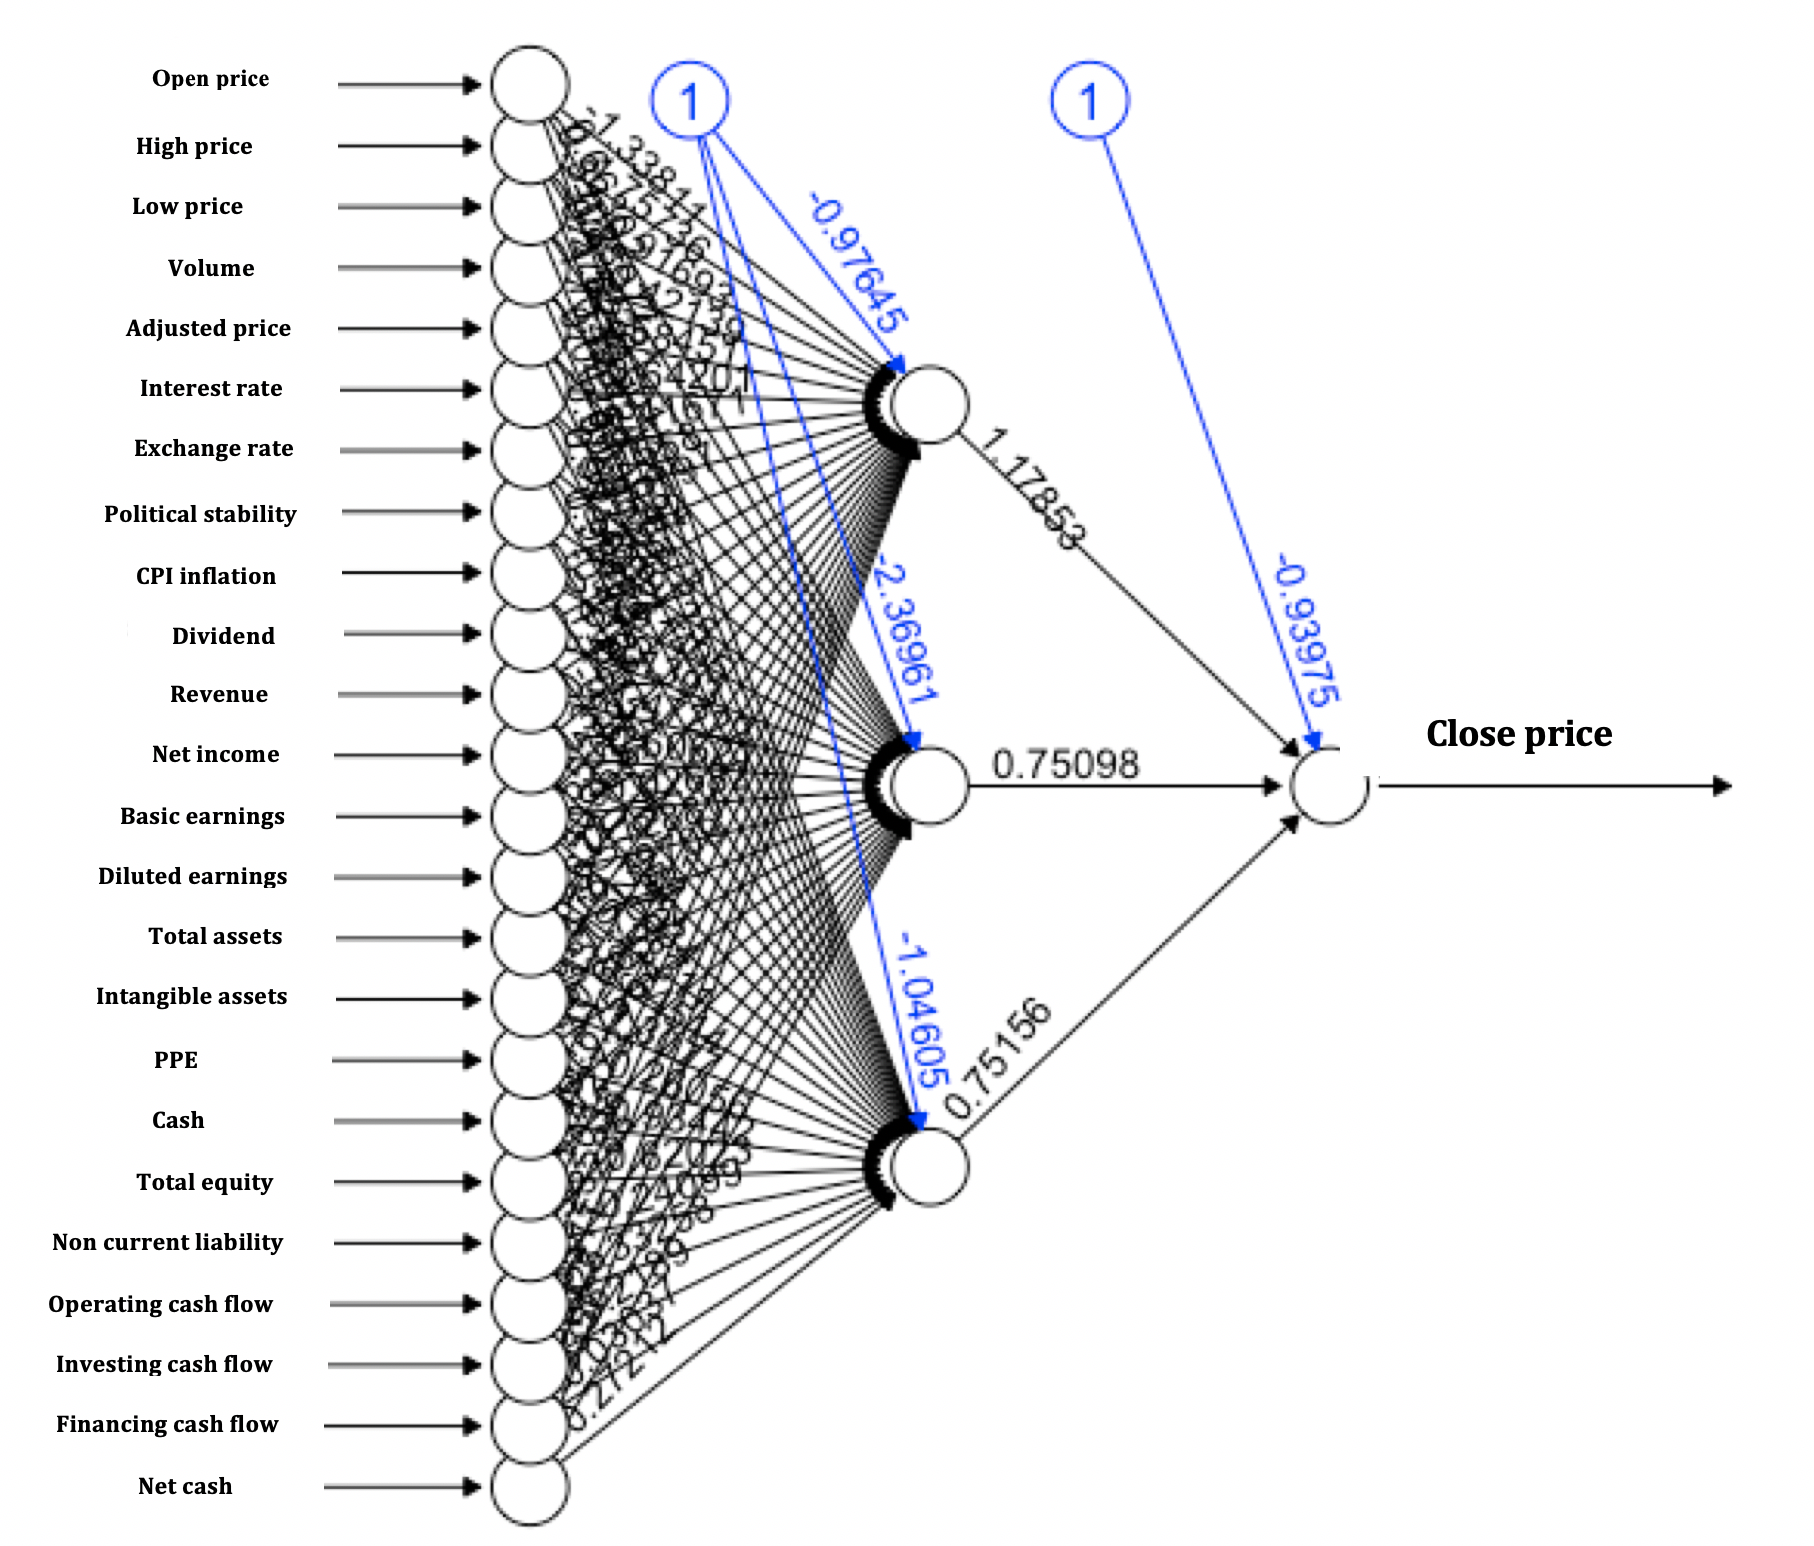
\includegraphics{D:/2017-2018/data_analysis/technical_analysis/report/NNrep.png}
\caption{Neuronal net representation}
\end{figure}

\begin{Shaded}
\begin{Highlighting}[]
\NormalTok{predict_testNN =}\StringTok{ }\KeywordTok{compute}\NormalTok{(NN, testNN[,}\KeywordTok{c}\NormalTok{(}\DecValTok{2}\OperatorTok{:}\DecValTok{25}\NormalTok{)])}
\CommentTok{# We descale the output to obtain the results in the real scale}
\NormalTok{predict_testNN =}\StringTok{ }\NormalTok{(predict_testNN}\OperatorTok{$}\NormalTok{net.result }\OperatorTok{*}\StringTok{ }\NormalTok{(}\KeywordTok{max}\NormalTok{(data}\OperatorTok{$}\NormalTok{A1) }\OperatorTok{-}\StringTok{ }\KeywordTok{min}\NormalTok{(data}\OperatorTok{$}\NormalTok{A1)))}
\OperatorTok{+}\StringTok{ }\KeywordTok{min}\NormalTok{(data}\OperatorTok{$}\NormalTok{A1)}
\CommentTok{# We create an array where to store the results per day for each stck}
\NormalTok{AI.P <-}\StringTok{ }\KeywordTok{c}\NormalTok{()}
\CommentTok{# We run the model for every single day per stock, to predict the prices }
\CommentTok{# one by one}
\KeywordTok{View}\NormalTok{(predict_testNN)}
\ControlFlowTok{for}\NormalTok{ (n }\ControlFlowTok{in} \DecValTok{1}\OperatorTok{:}\DecValTok{30}\NormalTok{)\{}
\NormalTok{  datatrain =}\StringTok{ }\NormalTok{data[ }\DecValTok{1}\OperatorTok{:}\DecValTok{1501}\OperatorTok{+}\NormalTok{n, ]}
\NormalTok{  datatest =}\StringTok{ }\NormalTok{data[ }\DecValTok{1502}\OperatorTok{+}\NormalTok{n, ]}
\NormalTok{  max =}\StringTok{ }\KeywordTok{apply}\NormalTok{(data , }\DecValTok{2}\NormalTok{ , max)}
\NormalTok{  min =}\StringTok{ }\KeywordTok{apply}\NormalTok{(data, }\DecValTok{2}\NormalTok{ , min)}
\NormalTok{  scaled =}\StringTok{ }\KeywordTok{as.data.frame}\NormalTok{(}\KeywordTok{scale}\NormalTok{(data, }\DataTypeTok{center =}\NormalTok{ min, }\DataTypeTok{scale =}\NormalTok{ max }\OperatorTok{-}\StringTok{ }\NormalTok{min))}
\NormalTok{  trainNN =}\StringTok{ }\NormalTok{scaled[}\DecValTok{1}\OperatorTok{:}\DecValTok{1501}\OperatorTok{+}\NormalTok{n , ]}
\NormalTok{  testNN =}\StringTok{ }\NormalTok{scaled[}\DecValTok{1502}\OperatorTok{+}\NormalTok{n , ]}
\CommentTok{# model with financial statements data}
\NormalTok{  NN =}\StringTok{ }\KeywordTok{neuralnet}\NormalTok{(A1 }\OperatorTok{~}\StringTok{ }\NormalTok{A2 }\OperatorTok{+}\StringTok{ }\NormalTok{A3 }\OperatorTok{+}\StringTok{ }\NormalTok{A4 }\OperatorTok{+}\StringTok{ }\NormalTok{A5 }\OperatorTok{+}\StringTok{ }\NormalTok{A6 }\OperatorTok{+}\StringTok{ }\NormalTok{A7 }\OperatorTok{+}\StringTok{ }\NormalTok{A8 }\OperatorTok{+}\StringTok{ }\NormalTok{A9 }\OperatorTok{+}\StringTok{ }\NormalTok{A10}
  \OperatorTok{+}\StringTok{ }\NormalTok{A11 }\OperatorTok{+}\StringTok{ }\NormalTok{A12 }\OperatorTok{+}\StringTok{ }\NormalTok{A13 }\OperatorTok{+}\StringTok{ }\NormalTok{A14 }\OperatorTok{+}\StringTok{ }\NormalTok{A15 }\OperatorTok{+}\StringTok{ }\NormalTok{A16 }\OperatorTok{+}\StringTok{ }\NormalTok{A17 }\OperatorTok{+}\StringTok{ }\NormalTok{A18 }\OperatorTok{+}\StringTok{ }\NormalTok{A19 }\OperatorTok{+}\StringTok{ }\NormalTok{A20 }\OperatorTok{+}\StringTok{ }\NormalTok{A21}
  \OperatorTok{+}\StringTok{ }\NormalTok{A22 }\OperatorTok{+}\StringTok{ }\NormalTok{A23 }\OperatorTok{+}\StringTok{ }\NormalTok{A24 }\OperatorTok{+}\StringTok{ }\NormalTok{A25, trainNN, }\DataTypeTok{hidden =} \DecValTok{3}\NormalTok{ , }\DataTypeTok{linear.output =}\NormalTok{ T )}
\NormalTok{  predict_testNN =}\StringTok{ }\KeywordTok{compute}\NormalTok{(NN, testNN[,}\KeywordTok{c}\NormalTok{(}\DecValTok{2}\OperatorTok{:}\DecValTok{25}\NormalTok{)])}
\NormalTok{  predict_testNN =}\StringTok{ }\NormalTok{(predict_testNN}\OperatorTok{$}\NormalTok{net.result }\OperatorTok{*}\StringTok{ }\NormalTok{(}\KeywordTok{max}\NormalTok{(data}\OperatorTok{$}\NormalTok{A1) }\OperatorTok{-}\StringTok{ }\KeywordTok{min}\NormalTok{(data}\OperatorTok{$}\NormalTok{A1)))}
  \OperatorTok{+}\StringTok{ }\KeywordTok{min}\NormalTok{(data}\OperatorTok{$}\NormalTok{A1)}
\NormalTok{  AI.P[n] <-}\StringTok{ }\NormalTok{predict_testNN}
\NormalTok{\}}
\NormalTok{AI.P2 <-}\StringTok{ }\KeywordTok{c}\NormalTok{()}
\ControlFlowTok{for}\NormalTok{ (n }\ControlFlowTok{in} \DecValTok{1}\OperatorTok{:}\DecValTok{30}\NormalTok{)\{}
\NormalTok{  datatrain =}\StringTok{ }\NormalTok{data[ }\DecValTok{1}\OperatorTok{:}\DecValTok{1501}\OperatorTok{+}\NormalTok{n, ]}
\NormalTok{  datatest =}\StringTok{ }\NormalTok{data[ }\DecValTok{1502}\OperatorTok{+}\NormalTok{n, ]}
\NormalTok{  max =}\StringTok{ }\KeywordTok{apply}\NormalTok{(data , }\DecValTok{2}\NormalTok{ , max)}
\NormalTok{  min =}\StringTok{ }\KeywordTok{apply}\NormalTok{(data, }\DecValTok{2}\NormalTok{ , min)}
\NormalTok{  scaled =}\StringTok{ }\KeywordTok{as.data.frame}\NormalTok{(}\KeywordTok{scale}\NormalTok{(data, }\DataTypeTok{center =}\NormalTok{ min, }\DataTypeTok{scale =}\NormalTok{ max }\OperatorTok{-}\StringTok{ }\NormalTok{min))}
\NormalTok{  trainNN =}\StringTok{ }\NormalTok{scaled[}\DecValTok{1}\OperatorTok{:}\DecValTok{1501}\OperatorTok{+}\NormalTok{n , ]}
\NormalTok{  testNN =}\StringTok{ }\NormalTok{scaled[}\DecValTok{1502}\OperatorTok{+}\NormalTok{n , ]}
\CommentTok{# model without financial statements data}
\NormalTok{  NN =}\StringTok{ }\KeywordTok{neuralnet}\NormalTok{(A1 }\OperatorTok{~}\StringTok{ }\NormalTok{A2 }\OperatorTok{+}\StringTok{ }\NormalTok{A3 }\OperatorTok{+}\StringTok{ }\NormalTok{A4 }\OperatorTok{+}\StringTok{ }\NormalTok{A5 }\OperatorTok{+}\StringTok{ }\NormalTok{A6 }\OperatorTok{+}\StringTok{ }\NormalTok{A7 }\OperatorTok{+}\StringTok{ }\NormalTok{A8 }\OperatorTok{+}\StringTok{ }\NormalTok{A9 }\OperatorTok{+}\StringTok{ }\NormalTok{A10,}
\NormalTok{  trainNN, }\DataTypeTok{hidden =} \DecValTok{3}\NormalTok{ , }\DataTypeTok{linear.output =}\NormalTok{ T )}
\NormalTok{  predict_testNN =}\StringTok{ }\KeywordTok{compute}\NormalTok{(NN, testNN[,}\KeywordTok{c}\NormalTok{(}\DecValTok{2}\OperatorTok{:}\DecValTok{10}\NormalTok{)])}
\NormalTok{  predict_testNN =}\StringTok{ }\NormalTok{(predict_testNN}\OperatorTok{$}\NormalTok{net.result }\OperatorTok{*}\StringTok{ }\NormalTok{(}\KeywordTok{max}\NormalTok{(data}\OperatorTok{$}\NormalTok{A1) }\OperatorTok{-}\StringTok{ }\KeywordTok{min}\NormalTok{(data}\OperatorTok{$}\NormalTok{A1)))}
  \OperatorTok{+}\StringTok{ }\KeywordTok{min}\NormalTok{(data}\OperatorTok{$}\NormalTok{A1)}
\NormalTok{  AI.P2[n] <-}\StringTok{ }\NormalTok{predict_testNN}
\NormalTok{\}}
\CommentTok{# Calculate Root Mean Square Error (RMSE)}
\NormalTok{Reals <-}\StringTok{ }\NormalTok{data[}\DecValTok{1503}\OperatorTok{:}\DecValTok{1532}\NormalTok{,}\DecValTok{1}\NormalTok{]}
\NormalTok{RMSE <-}\StringTok{ }\KeywordTok{sqrt}\NormalTok{(}\KeywordTok{sum}\NormalTok{((Reals}\OperatorTok{-}\NormalTok{AI.P)}\OperatorTok{^}\DecValTok{2}\NormalTok{)) }\CommentTok{# RMSE = 6.072}
\NormalTok{RMSE2 <-}\StringTok{ }\KeywordTok{sqrt}\NormalTok{(}\KeywordTok{sum}\NormalTok{((Reals}\OperatorTok{-}\NormalTok{AI.P2)}\OperatorTok{^}\DecValTok{2}\NormalTok{)) }\CommentTok{# RMSE2 = 6.064}
\end{Highlighting}
\end{Shaded}

As can be seen, the model without the financial statement variables
(RMSE = 6.072) is more accurate than the model with them (RMSE2 = 6.064)
according to the RMSE value. Hence, we will continue without taking into
account the financial statement variables.

\begin{Shaded}
\begin{Highlighting}[]
\CommentTok{#We predict the prices of the other 4 stocks one by one,}
\CommentTok{#without the financial statement variables as input}
\KeywordTok{library}\NormalTok{(readr)}
\NormalTok{AIR1 <-}\StringTok{ }\KeywordTok{read_csv2}\NormalTok{(}\StringTok{"D:/2017-2018/data_analysis/technical_analysis/data/AIR1.csv"}\NormalTok{)}
\NormalTok{data <-}\StringTok{ }\NormalTok{AIR1}
\NormalTok{AIR.P2 <-}\StringTok{ }\KeywordTok{c}\NormalTok{()}
\ControlFlowTok{for}\NormalTok{ (n }\ControlFlowTok{in} \DecValTok{1}\OperatorTok{:}\DecValTok{30}\NormalTok{)\{}
\NormalTok{  datatrain =}\StringTok{ }\NormalTok{data[ }\DecValTok{1}\OperatorTok{:}\DecValTok{1501}\OperatorTok{+}\NormalTok{n, ]}
\NormalTok{  datatest =}\StringTok{ }\NormalTok{data[ }\DecValTok{1502}\OperatorTok{+}\NormalTok{n, ]}
\NormalTok{  max =}\StringTok{ }\KeywordTok{apply}\NormalTok{(data , }\DecValTok{2}\NormalTok{ , max)}
\NormalTok{  min =}\StringTok{ }\KeywordTok{apply}\NormalTok{(data, }\DecValTok{2}\NormalTok{ , min)}
\NormalTok{  scaled =}\StringTok{ }\KeywordTok{as.data.frame}\NormalTok{(}\KeywordTok{scale}\NormalTok{(data, }\DataTypeTok{center =}\NormalTok{ min, }\DataTypeTok{scale =}\NormalTok{ max }\OperatorTok{-}\StringTok{ }\NormalTok{min))}
\NormalTok{  trainNN =}\StringTok{ }\NormalTok{scaled[}\DecValTok{1}\OperatorTok{:}\DecValTok{1501}\OperatorTok{+}\NormalTok{n , ]}
\NormalTok{  testNN =}\StringTok{ }\NormalTok{scaled[}\DecValTok{1502}\OperatorTok{+}\NormalTok{n , ]}
\NormalTok{  NN =}\StringTok{ }\KeywordTok{neuralnet}\NormalTok{(A1 }\OperatorTok{~}\StringTok{ }\NormalTok{A2 }\OperatorTok{+}\StringTok{ }\NormalTok{A3 }\OperatorTok{+}\StringTok{ }\NormalTok{A4 }\OperatorTok{+}\StringTok{ }\NormalTok{A5 }\OperatorTok{+}\StringTok{ }\NormalTok{A6 }\OperatorTok{+}\StringTok{ }\NormalTok{A7 }\OperatorTok{+}\StringTok{ }\NormalTok{A8 }\OperatorTok{+}\StringTok{ }\NormalTok{A9 }\OperatorTok{+}\StringTok{ }\NormalTok{A10,}
\NormalTok{  trainNN, }\DataTypeTok{hidden =} \DecValTok{3}\NormalTok{ , }\DataTypeTok{linear.output =}\NormalTok{ T )}
\NormalTok{  predict_testNN =}\StringTok{ }\KeywordTok{compute}\NormalTok{(NN, testNN[,}\KeywordTok{c}\NormalTok{(}\DecValTok{2}\OperatorTok{:}\DecValTok{10}\NormalTok{)])}
\NormalTok{  predict_testNN =}\StringTok{ }\NormalTok{(predict_testNN}\OperatorTok{$}\NormalTok{net.result }\OperatorTok{*}\StringTok{ }\NormalTok{(}\KeywordTok{max}\NormalTok{(data}\OperatorTok{$}\NormalTok{A1) }\OperatorTok{-}\StringTok{ }\KeywordTok{min}\NormalTok{(data}\OperatorTok{$}\NormalTok{A1)))}
  \OperatorTok{+}\StringTok{ }\KeywordTok{min}\NormalTok{(data}\OperatorTok{$}\NormalTok{A1)}
\NormalTok{  AIR.P2[n] <-}\StringTok{ }\NormalTok{predict_testNN}
\NormalTok{\}}
\CommentTok{#We run the same for loop above also for BN.PA, BNP.PA and DG.PA}
\end{Highlighting}
\end{Shaded}

We want to create a table with the predicted daily increase in price for
every stock during the 30 days. After that, we will identify the stock
with the highest predicted increase in price for every day. This will be
the stock where to invest all the capital for the day.

\begin{Shaded}
\begin{Highlighting}[]
\NormalTok{AI.R <-}\StringTok{ }\NormalTok{AI1[}\DecValTok{1502}\OperatorTok{:}\DecValTok{1531}\NormalTok{, }\KeywordTok{c}\NormalTok{(}\DecValTok{2}\NormalTok{)]}
\NormalTok{AIR.R <-}\StringTok{ }\NormalTok{AIR1[}\DecValTok{1502}\OperatorTok{:}\DecValTok{1531}\NormalTok{, }\KeywordTok{c}\NormalTok{(}\DecValTok{1}\NormalTok{)]}
\NormalTok{BN.R <-}\StringTok{ }\NormalTok{BN1[}\DecValTok{1502}\OperatorTok{:}\DecValTok{1531}\NormalTok{, }\KeywordTok{c}\NormalTok{(}\DecValTok{1}\NormalTok{)]}
\NormalTok{BNP.R <-}\StringTok{ }\NormalTok{BNP1[}\DecValTok{1502}\OperatorTok{:}\DecValTok{1531}\NormalTok{, }\KeywordTok{c}\NormalTok{(}\DecValTok{1}\NormalTok{)]}
\NormalTok{DG.R <-}\StringTok{ }\NormalTok{DG1[}\DecValTok{1502}\OperatorTok{:}\DecValTok{1531}\NormalTok{, }\KeywordTok{c}\NormalTok{(}\DecValTok{1}\NormalTok{)]}
\NormalTok{AI.DIF <-}\StringTok{ }\NormalTok{AI.P2 }\OperatorTok{-}\StringTok{ }\NormalTok{AI.R}
\NormalTok{AIR.DIF <-}\StringTok{ }\NormalTok{AIR.P2 }\OperatorTok{-}\StringTok{ }\NormalTok{AIR.R}
\NormalTok{BN.DIF <-}\StringTok{ }\NormalTok{BN.P2 }\OperatorTok{-}\StringTok{ }\NormalTok{BN.R}
\NormalTok{BNP.DIF <-}\StringTok{ }\NormalTok{BNP.P2 }\OperatorTok{-}\StringTok{ }\NormalTok{BNP.R}
\NormalTok{DG.DIF <-}\StringTok{ }\NormalTok{DG.P2 }\OperatorTok{-}\StringTok{ }\NormalTok{DG.R}
\NormalTok{df =}\StringTok{ }\KeywordTok{data.frame}\NormalTok{(AI.DIF,AIR.DIF,BN.DIF,BNP.DIF,DG.DIF)}
\CommentTok{#identify the stock with the highest predicted increase in price for every day}
\NormalTok{X <-}\StringTok{ }\KeywordTok{c}\NormalTok{()}
\ControlFlowTok{for}\NormalTok{ (n }\ControlFlowTok{in} \DecValTok{1}\OperatorTok{:}\DecValTok{30}\NormalTok{)\{}
  \ControlFlowTok{if}\NormalTok{ (}\KeywordTok{max}\NormalTok{(df[n,]) }\OperatorTok{==}\StringTok{ }\NormalTok{df[n,}\StringTok{"A1"}\NormalTok{])\{}
\NormalTok{    X[n] =}\StringTok{ "AI.PA"}
\NormalTok{  \} }\ControlFlowTok{else} \ControlFlowTok{if}\NormalTok{ (}\KeywordTok{max}\NormalTok{(df[n,]) }\OperatorTok{==}\StringTok{ }\NormalTok{df[n,}\StringTok{"A1.1"}\NormalTok{])\{}
\NormalTok{    X[n] =}\StringTok{ "AIR.PA"}
\NormalTok{  \} }\ControlFlowTok{else} \ControlFlowTok{if}\NormalTok{ (}\KeywordTok{max}\NormalTok{(df[n,]) }\OperatorTok{==}\StringTok{ }\NormalTok{df[n,}\StringTok{"A1.2"}\NormalTok{])\{}
\NormalTok{    X[n] =}\StringTok{ "BN.PA"}
\NormalTok{  \} }\ControlFlowTok{else} \ControlFlowTok{if}\NormalTok{ (}\KeywordTok{max}\NormalTok{(df[n,]) }\OperatorTok{==}\StringTok{ }\NormalTok{df[n,}\StringTok{"A1.3"}\NormalTok{])\{}
\NormalTok{    X[n] =}\StringTok{ "BNP.PA"}
\NormalTok{  \} }\ControlFlowTok{else} \ControlFlowTok{if}\NormalTok{ (}\KeywordTok{max}\NormalTok{(df[n,]) }\OperatorTok{==}\StringTok{ }\NormalTok{df[n,}\StringTok{"A1.4"}\NormalTok{])\{}
\NormalTok{    X[n] =}\StringTok{ "DG.PA"}
\NormalTok{  \}}
\NormalTok{\}}
\end{Highlighting}
\end{Shaded}

\begin{longtable}[]{@{}llllllllll@{}}
\caption{Multiple-input NN strategy outcome}\tabularnewline
\toprule
\begin{minipage}[b]{0.04\columnwidth}\raggedright
Day\strut
\end{minipage} & \begin{minipage}[b]{0.09\columnwidth}\raggedright
Invest in\strut
\end{minipage} & \begin{minipage}[b]{0.10\columnwidth}\raggedright
date\strut
\end{minipage} & \begin{minipage}[b]{0.06\columnwidth}\raggedright
AI\strut
\end{minipage} & \begin{minipage}[b]{0.06\columnwidth}\raggedright
AIR\strut
\end{minipage} & \begin{minipage}[b]{0.06\columnwidth}\raggedright
BNP\strut
\end{minipage} & \begin{minipage}[b]{0.06\columnwidth}\raggedright
BN\strut
\end{minipage} & \begin{minipage}[b]{0.06\columnwidth}\raggedright
DG\strut
\end{minipage} & \begin{minipage}[b]{0.13\columnwidth}\raggedright
\#shares bought\strut
\end{minipage} & \begin{minipage}[b]{0.08\columnwidth}\raggedright
€ Value\strut
\end{minipage}\tabularnewline
\midrule
\endfirsthead
\toprule
\begin{minipage}[b]{0.04\columnwidth}\raggedright
Day\strut
\end{minipage} & \begin{minipage}[b]{0.09\columnwidth}\raggedright
Invest in\strut
\end{minipage} & \begin{minipage}[b]{0.10\columnwidth}\raggedright
date\strut
\end{minipage} & \begin{minipage}[b]{0.06\columnwidth}\raggedright
AI\strut
\end{minipage} & \begin{minipage}[b]{0.06\columnwidth}\raggedright
AIR\strut
\end{minipage} & \begin{minipage}[b]{0.06\columnwidth}\raggedright
BNP\strut
\end{minipage} & \begin{minipage}[b]{0.06\columnwidth}\raggedright
BN\strut
\end{minipage} & \begin{minipage}[b]{0.06\columnwidth}\raggedright
DG\strut
\end{minipage} & \begin{minipage}[b]{0.13\columnwidth}\raggedright
\#shares bought\strut
\end{minipage} & \begin{minipage}[b]{0.08\columnwidth}\raggedright
€ Value\strut
\end{minipage}\tabularnewline
\midrule
\endhead
\begin{minipage}[t]{0.04\columnwidth}\raggedright
1\strut
\end{minipage} & \begin{minipage}[t]{0.09\columnwidth}\raggedright
DG\strut
\end{minipage} & \begin{minipage}[t]{0.10\columnwidth}\raggedright
16/11/2018\strut
\end{minipage} & \begin{minipage}[t]{0.06\columnwidth}\raggedright
95.86\strut
\end{minipage} & \begin{minipage}[t]{0.06\columnwidth}\raggedright
92.88\strut
\end{minipage} & \begin{minipage}[t]{0.06\columnwidth}\raggedright
65.09\strut
\end{minipage} & \begin{minipage}[t]{0.06\columnwidth}\raggedright
45.19\strut
\end{minipage} & \begin{minipage}[t]{0.06\columnwidth}\raggedright
77.09\strut
\end{minipage} & \begin{minipage}[t]{0.13\columnwidth}\raggedright
129.70\strut
\end{minipage} & \begin{minipage}[t]{0.08\columnwidth}\raggedright
10000\strut
\end{minipage}\tabularnewline
\begin{minipage}[t]{0.04\columnwidth}\raggedright
2\strut
\end{minipage} & \begin{minipage}[t]{0.09\columnwidth}\raggedright
DG\strut
\end{minipage} & \begin{minipage}[t]{0.10\columnwidth}\raggedright
19/11/2018\strut
\end{minipage} & \begin{minipage}[t]{0.06\columnwidth}\raggedright
95.40\strut
\end{minipage} & \begin{minipage}[t]{0.06\columnwidth}\raggedright
92.57\strut
\end{minipage} & \begin{minipage}[t]{0.06\columnwidth}\raggedright
64.70\strut
\end{minipage} & \begin{minipage}[t]{0.06\columnwidth}\raggedright
45.28\strut
\end{minipage} & \begin{minipage}[t]{0.06\columnwidth}\raggedright
76.80\strut
\end{minipage} & \begin{minipage}[t]{0.13\columnwidth}\raggedright
129.70\strut
\end{minipage} & \begin{minipage}[t]{0.08\columnwidth}\raggedright
9961.09\strut
\end{minipage}\tabularnewline
\begin{minipage}[t]{0.04\columnwidth}\raggedright
3\strut
\end{minipage} & \begin{minipage}[t]{0.09\columnwidth}\raggedright
DG\strut
\end{minipage} & \begin{minipage}[t]{0.10\columnwidth}\raggedright
20/11/2018\strut
\end{minipage} & \begin{minipage}[t]{0.06\columnwidth}\raggedright
93.5\strut
\end{minipage} & \begin{minipage}[t]{0.06\columnwidth}\raggedright
91.07\strut
\end{minipage} & \begin{minipage}[t]{0.06\columnwidth}\raggedright
64.98\strut
\end{minipage} & \begin{minipage}[t]{0.06\columnwidth}\raggedright
44.30\strut
\end{minipage} & \begin{minipage}[t]{0.06\columnwidth}\raggedright
76.37\strut
\end{minipage} & \begin{minipage}[t]{0.13\columnwidth}\raggedright
129.70\strut
\end{minipage} & \begin{minipage}[t]{0.08\columnwidth}\raggedright
9906.61\strut
\end{minipage}\tabularnewline
\begin{minipage}[t]{0.04\columnwidth}\raggedright
4\strut
\end{minipage} & \begin{minipage}[t]{0.09\columnwidth}\raggedright
AIR\strut
\end{minipage} & \begin{minipage}[t]{0.10\columnwidth}\raggedright
21/11/2018\strut
\end{minipage} & \begin{minipage}[t]{0.06\columnwidth}\raggedright
94.22\strut
\end{minipage} & \begin{minipage}[t]{0.06\columnwidth}\raggedright
93.16\strut
\end{minipage} & \begin{minipage}[t]{0.06\columnwidth}\raggedright
65.41\strut
\end{minipage} & \begin{minipage}[t]{0.06\columnwidth}\raggedright
44.79\strut
\end{minipage} & \begin{minipage}[t]{0.06\columnwidth}\raggedright
77.01\strut
\end{minipage} & \begin{minipage}[t]{0.13\columnwidth}\raggedright
107.21\strut
\end{minipage} & \begin{minipage}[t]{0.08\columnwidth}\raggedright
9989.62\strut
\end{minipage}\tabularnewline
\begin{minipage}[t]{0.04\columnwidth}\raggedright
5\strut
\end{minipage} & \begin{minipage}[t]{0.09\columnwidth}\raggedright
AIR\strut
\end{minipage} & \begin{minipage}[t]{0.10\columnwidth}\raggedright
22/11/2018\strut
\end{minipage} & \begin{minipage}[t]{0.06\columnwidth}\raggedright
93.31\strut
\end{minipage} & \begin{minipage}[t]{0.06\columnwidth}\raggedright
92.33\strut
\end{minipage} & \begin{minipage}[t]{0.06\columnwidth}\raggedright
65.27\strut
\end{minipage} & \begin{minipage}[t]{0.06\columnwidth}\raggedright
44.28\strut
\end{minipage} & \begin{minipage}[t]{0.06\columnwidth}\raggedright
76.62\strut
\end{minipage} & \begin{minipage}[t]{0.13\columnwidth}\raggedright
107.21\strut
\end{minipage} & \begin{minipage}[t]{0.08\columnwidth}\raggedright
9899.55\strut
\end{minipage}\tabularnewline
\begin{minipage}[t]{0.04\columnwidth}\raggedright
6\strut
\end{minipage} & \begin{minipage}[t]{0.09\columnwidth}\raggedright
DG\strut
\end{minipage} & \begin{minipage}[t]{0.10\columnwidth}\raggedright
23/11/2018\strut
\end{minipage} & \begin{minipage}[t]{0.06\columnwidth}\raggedright
93.86\strut
\end{minipage} & \begin{minipage}[t]{0.06\columnwidth}\raggedright
93.41\strut
\end{minipage} & \begin{minipage}[t]{0.06\columnwidth}\raggedright
65.87\strut
\end{minipage} & \begin{minipage}[t]{0.06\columnwidth}\raggedright
44.36\strut
\end{minipage} & \begin{minipage}[t]{0.06\columnwidth}\raggedright
76.86\strut
\end{minipage} & \begin{minipage}[t]{0.13\columnwidth}\raggedright
130.30\strut
\end{minipage} & \begin{minipage}[t]{0.08\columnwidth}\raggedright
10015.35\strut
\end{minipage}\tabularnewline
\begin{minipage}[t]{0.04\columnwidth}\raggedright
7\strut
\end{minipage} & \begin{minipage}[t]{0.09\columnwidth}\raggedright
DG\strut
\end{minipage} & \begin{minipage}[t]{0.10\columnwidth}\raggedright
26/11/2018\strut
\end{minipage} & \begin{minipage}[t]{0.06\columnwidth}\raggedright
95.86\strut
\end{minipage} & \begin{minipage}[t]{0.06\columnwidth}\raggedright
93.58\strut
\end{minipage} & \begin{minipage}[t]{0.06\columnwidth}\raggedright
65.82\strut
\end{minipage} & \begin{minipage}[t]{0.06\columnwidth}\raggedright
45.34\strut
\end{minipage} & \begin{minipage}[t]{0.06\columnwidth}\raggedright
78.54\strut
\end{minipage} & \begin{minipage}[t]{0.13\columnwidth}\raggedright
130.30\strut
\end{minipage} & \begin{minipage}[t]{0.08\columnwidth}\raggedright
10234.27\strut
\end{minipage}\tabularnewline
\begin{minipage}[t]{0.04\columnwidth}\raggedright
8\strut
\end{minipage} & \begin{minipage}[t]{0.09\columnwidth}\raggedright
AIR\strut
\end{minipage} & \begin{minipage}[t]{0.10\columnwidth}\raggedright
27/11/2018\strut
\end{minipage} & \begin{minipage}[t]{0.06\columnwidth}\raggedright
94.86\strut
\end{minipage} & \begin{minipage}[t]{0.06\columnwidth}\raggedright
93.69\strut
\end{minipage} & \begin{minipage}[t]{0.06\columnwidth}\raggedright
66.41\strut
\end{minipage} & \begin{minipage}[t]{0.06\columnwidth}\raggedright
45.08\strut
\end{minipage} & \begin{minipage}[t]{0.06\columnwidth}\raggedright
78.16\strut
\end{minipage} & \begin{minipage}[t]{0.13\columnwidth}\raggedright
108.69\strut
\end{minipage} & \begin{minipage}[t]{0.08\columnwidth}\raggedright
10184.75\strut
\end{minipage}\tabularnewline
\begin{minipage}[t]{0.04\columnwidth}\raggedright
9\strut
\end{minipage} & \begin{minipage}[t]{0.09\columnwidth}\raggedright
DG\strut
\end{minipage} & \begin{minipage}[t]{0.10\columnwidth}\raggedright
28/11/2018\strut
\end{minipage} & \begin{minipage}[t]{0.06\columnwidth}\raggedright
94.36\strut
\end{minipage} & \begin{minipage}[t]{0.06\columnwidth}\raggedright
93.5\strut
\end{minipage} & \begin{minipage}[t]{0.06\columnwidth}\raggedright
65.41\strut
\end{minipage} & \begin{minipage}[t]{0.06\columnwidth}\raggedright
44.75\strut
\end{minipage} & \begin{minipage}[t]{0.06\columnwidth}\raggedright
77.95\strut
\end{minipage} & \begin{minipage}[t]{0.13\columnwidth}\raggedright
130.36\strut
\end{minipage} & \begin{minipage}[t]{0.08\columnwidth}\raggedright
10163.01\strut
\end{minipage}\tabularnewline
\begin{minipage}[t]{0.04\columnwidth}\raggedright
10\strut
\end{minipage} & \begin{minipage}[t]{0.09\columnwidth}\raggedright
DG\strut
\end{minipage} & \begin{minipage}[t]{0.10\columnwidth}\raggedright
29/11/2018\strut
\end{minipage} & \begin{minipage}[t]{0.06\columnwidth}\raggedright
94.68\strut
\end{minipage} & \begin{minipage}[t]{0.06\columnwidth}\raggedright
94.86\strut
\end{minipage} & \begin{minipage}[t]{0.06\columnwidth}\raggedright
65.54\strut
\end{minipage} & \begin{minipage}[t]{0.06\columnwidth}\raggedright
44.77\strut
\end{minipage} & \begin{minipage}[t]{0.06\columnwidth}\raggedright
77.58\strut
\end{minipage} & \begin{minipage}[t]{0.13\columnwidth}\raggedright
130.36\strut
\end{minipage} & \begin{minipage}[t]{0.08\columnwidth}\raggedright
10113.47\strut
\end{minipage}\tabularnewline
\begin{minipage}[t]{0.04\columnwidth}\raggedright
11\strut
\end{minipage} & \begin{minipage}[t]{0.09\columnwidth}\raggedright
DG\strut
\end{minipage} & \begin{minipage}[t]{0.10\columnwidth}\raggedright
30/11/2018\strut
\end{minipage} & \begin{minipage}[t]{0.06\columnwidth}\raggedright
97.04\strut
\end{minipage} & \begin{minipage}[t]{0.06\columnwidth}\raggedright
94.62\strut
\end{minipage} & \begin{minipage}[t]{0.06\columnwidth}\raggedright
66.05\strut
\end{minipage} & \begin{minipage}[t]{0.06\columnwidth}\raggedright
44.37\strut
\end{minipage} & \begin{minipage}[t]{0.06\columnwidth}\raggedright
77.09\strut
\end{minipage} & \begin{minipage}[t]{0.13\columnwidth}\raggedright
130.36\strut
\end{minipage} & \begin{minipage}[t]{0.08\columnwidth}\raggedright
10050.90\strut
\end{minipage}\tabularnewline
\begin{minipage}[t]{0.04\columnwidth}\raggedright
12\strut
\end{minipage} & \begin{minipage}[t]{0.09\columnwidth}\raggedright
DG\strut
\end{minipage} & \begin{minipage}[t]{0.10\columnwidth}\raggedright
03/12/2018\strut
\end{minipage} & \begin{minipage}[t]{0.06\columnwidth}\raggedright
97.27\strut
\end{minipage} & \begin{minipage}[t]{0.06\columnwidth}\raggedright
95.69\strut
\end{minipage} & \begin{minipage}[t]{0.06\columnwidth}\raggedright
65.41\strut
\end{minipage} & \begin{minipage}[t]{0.06\columnwidth}\raggedright
44.84\strut
\end{minipage} & \begin{minipage}[t]{0.06\columnwidth}\raggedright
75.40\strut
\end{minipage} & \begin{minipage}[t]{0.13\columnwidth}\raggedright
130.36\strut
\end{minipage} & \begin{minipage}[t]{0.08\columnwidth}\raggedright
9829.29\strut
\end{minipage}\tabularnewline
\begin{minipage}[t]{0.04\columnwidth}\raggedright
13\strut
\end{minipage} & \begin{minipage}[t]{0.09\columnwidth}\raggedright
DG\strut
\end{minipage} & \begin{minipage}[t]{0.10\columnwidth}\raggedright
04/12/2018\strut
\end{minipage} & \begin{minipage}[t]{0.06\columnwidth}\raggedright
97.45\strut
\end{minipage} & \begin{minipage}[t]{0.06\columnwidth}\raggedright
94.26\strut
\end{minipage} & \begin{minipage}[t]{0.06\columnwidth}\raggedright
65.52\strut
\end{minipage} & \begin{minipage}[t]{0.06\columnwidth}\raggedright
43.86\strut
\end{minipage} & \begin{minipage}[t]{0.06\columnwidth}\raggedright
76.66\strut
\end{minipage} & \begin{minipage}[t]{0.13\columnwidth}\raggedright
130.36\strut
\end{minipage} & \begin{minipage}[t]{0.08\columnwidth}\raggedright
9993.54\strut
\end{minipage}\tabularnewline
\begin{minipage}[t]{0.04\columnwidth}\raggedright
14\strut
\end{minipage} & \begin{minipage}[t]{0.09\columnwidth}\raggedright
AIR\strut
\end{minipage} & \begin{minipage}[t]{0.10\columnwidth}\raggedright
05/12/2018\strut
\end{minipage} & \begin{minipage}[t]{0.06\columnwidth}\raggedright
96.45\strut
\end{minipage} & \begin{minipage}[t]{0.06\columnwidth}\raggedright
92.30\strut
\end{minipage} & \begin{minipage}[t]{0.06\columnwidth}\raggedright
64.58\strut
\end{minipage} & \begin{minipage}[t]{0.06\columnwidth}\raggedright
43.41\strut
\end{minipage} & \begin{minipage}[t]{0.06\columnwidth}\raggedright
74.66\strut
\end{minipage} & \begin{minipage}[t]{0.13\columnwidth}\raggedright
105.43\strut
\end{minipage} & \begin{minipage}[t]{0.08\columnwidth}\raggedright
9732.82\strut
\end{minipage}\tabularnewline
\begin{minipage}[t]{0.04\columnwidth}\raggedright
15\strut
\end{minipage} & \begin{minipage}[t]{0.09\columnwidth}\raggedright
DG\strut
\end{minipage} & \begin{minipage}[t]{0.10\columnwidth}\raggedright
06/12/2018\strut
\end{minipage} & \begin{minipage}[t]{0.06\columnwidth}\raggedright
94.63\strut
\end{minipage} & \begin{minipage}[t]{0.06\columnwidth}\raggedright
88.63\strut
\end{minipage} & \begin{minipage}[t]{0.06\columnwidth}\raggedright
63.43\strut
\end{minipage} & \begin{minipage}[t]{0.06\columnwidth}\raggedright
41.78\strut
\end{minipage} & \begin{minipage}[t]{0.06\columnwidth}\raggedright
70.98\strut
\end{minipage} & \begin{minipage}[t]{0.13\columnwidth}\raggedright
131.66\strut
\end{minipage} & \begin{minipage}[t]{0.08\columnwidth}\raggedright
9345.87\strut
\end{minipage}\tabularnewline
\begin{minipage}[t]{0.04\columnwidth}\raggedright
16\strut
\end{minipage} & \begin{minipage}[t]{0.09\columnwidth}\raggedright
DG\strut
\end{minipage} & \begin{minipage}[t]{0.10\columnwidth}\raggedright
07/12/2018\strut
\end{minipage} & \begin{minipage}[t]{0.06\columnwidth}\raggedright
95.86\strut
\end{minipage} & \begin{minipage}[t]{0.06\columnwidth}\raggedright
89.07\strut
\end{minipage} & \begin{minipage}[t]{0.06\columnwidth}\raggedright
63.79\strut
\end{minipage} & \begin{minipage}[t]{0.06\columnwidth}\raggedright
41.59\strut
\end{minipage} & \begin{minipage}[t]{0.06\columnwidth}\raggedright
72.68\strut
\end{minipage} & \begin{minipage}[t]{0.13\columnwidth}\raggedright
131.66\strut
\end{minipage} & \begin{minipage}[t]{0.08\columnwidth}\raggedright
9569.70\strut
\end{minipage}\tabularnewline
\begin{minipage}[t]{0.04\columnwidth}\raggedright
17\strut
\end{minipage} & \begin{minipage}[t]{0.09\columnwidth}\raggedright
AIR\strut
\end{minipage} & \begin{minipage}[t]{0.10\columnwidth}\raggedright
10/12/2018\strut
\end{minipage} & \begin{minipage}[t]{0.06\columnwidth}\raggedright
95.77\strut
\end{minipage} & \begin{minipage}[t]{0.06\columnwidth}\raggedright
87.48\strut
\end{minipage} & \begin{minipage}[t]{0.06\columnwidth}\raggedright
62.97\strut
\end{minipage} & \begin{minipage}[t]{0.06\columnwidth}\raggedright
40.40\strut
\end{minipage} & \begin{minipage}[t]{0.06\columnwidth}\raggedright
71.66\strut
\end{minipage} & \begin{minipage}[t]{0.13\columnwidth}\raggedright
107.84\strut
\end{minipage} & \begin{minipage}[t]{0.08\columnwidth}\raggedright
9435.40\strut
\end{minipage}\tabularnewline
\begin{minipage}[t]{0.04\columnwidth}\raggedright
18\strut
\end{minipage} & \begin{minipage}[t]{0.09\columnwidth}\raggedright
DG\strut
\end{minipage} & \begin{minipage}[t]{0.10\columnwidth}\raggedright
11/12/2018\strut
\end{minipage} & \begin{minipage}[t]{0.06\columnwidth}\raggedright
96.45\strut
\end{minipage} & \begin{minipage}[t]{0.06\columnwidth}\raggedright
88.59\strut
\end{minipage} & \begin{minipage}[t]{0.06\columnwidth}\raggedright
62.81\strut
\end{minipage} & \begin{minipage}[t]{0.06\columnwidth}\raggedright
40.68\strut
\end{minipage} & \begin{minipage}[t]{0.06\columnwidth}\raggedright
73.69\strut
\end{minipage} & \begin{minipage}[t]{0.13\columnwidth}\raggedright
129.64\strut
\end{minipage} & \begin{minipage}[t]{0.08\columnwidth}\raggedright
9555.11\strut
\end{minipage}\tabularnewline
\begin{minipage}[t]{0.04\columnwidth}\raggedright
19\strut
\end{minipage} & \begin{minipage}[t]{0.09\columnwidth}\raggedright
AI\strut
\end{minipage} & \begin{minipage}[t]{0.10\columnwidth}\raggedright
12/12/2018\strut
\end{minipage} & \begin{minipage}[t]{0.06\columnwidth}\raggedright
97.54\strut
\end{minipage} & \begin{minipage}[t]{0.06\columnwidth}\raggedright
91.48\strut
\end{minipage} & \begin{minipage}[t]{0.06\columnwidth}\raggedright
64.12\strut
\end{minipage} & \begin{minipage}[t]{0.06\columnwidth}\raggedright
41.90\strut
\end{minipage} & \begin{minipage}[t]{0.06\columnwidth}\raggedright
74.77\strut
\end{minipage} & \begin{minipage}[t]{0.13\columnwidth}\raggedright
99.39\strut
\end{minipage} & \begin{minipage}[t]{0.08\columnwidth}\raggedright
9695.13\strut
\end{minipage}\tabularnewline
\begin{minipage}[t]{0.04\columnwidth}\raggedright
20\strut
\end{minipage} & \begin{minipage}[t]{0.09\columnwidth}\raggedright
DG\strut
\end{minipage} & \begin{minipage}[t]{0.10\columnwidth}\raggedright
13/12/2018\strut
\end{minipage} & \begin{minipage}[t]{0.06\columnwidth}\raggedright
97.63\strut
\end{minipage} & \begin{minipage}[t]{0.06\columnwidth}\raggedright
89.97\strut
\end{minipage} & \begin{minipage}[t]{0.06\columnwidth}\raggedright
64.32\strut
\end{minipage} & \begin{minipage}[t]{0.06\columnwidth}\raggedright
42.18\strut
\end{minipage} & \begin{minipage}[t]{0.06\columnwidth}\raggedright
74.5\strut
\end{minipage} & \begin{minipage}[t]{0.13\columnwidth}\raggedright
130.25\strut
\end{minipage} & \begin{minipage}[t]{0.08\columnwidth}\raggedright
9704.18\strut
\end{minipage}\tabularnewline
\begin{minipage}[t]{0.04\columnwidth}\raggedright
21\strut
\end{minipage} & \begin{minipage}[t]{0.09\columnwidth}\raggedright
AIR\strut
\end{minipage} & \begin{minipage}[t]{0.10\columnwidth}\raggedright
14/12/2018\strut
\end{minipage} & \begin{minipage}[t]{0.06\columnwidth}\raggedright
97.45\strut
\end{minipage} & \begin{minipage}[t]{0.06\columnwidth}\raggedright
88.66\strut
\end{minipage} & \begin{minipage}[t]{0.06\columnwidth}\raggedright
64.08\strut
\end{minipage} & \begin{minipage}[t]{0.06\columnwidth}\raggedright
41.59\strut
\end{minipage} & \begin{minipage}[t]{0.06\columnwidth}\raggedright
73.51\strut
\end{minipage} & \begin{minipage}[t]{0.13\columnwidth}\raggedright
108.00\strut
\end{minipage} & \begin{minipage}[t]{0.08\columnwidth}\raggedright
9576.52\strut
\end{minipage}\tabularnewline
\begin{minipage}[t]{0.04\columnwidth}\raggedright
22\strut
\end{minipage} & \begin{minipage}[t]{0.09\columnwidth}\raggedright
AIR\strut
\end{minipage} & \begin{minipage}[t]{0.10\columnwidth}\raggedright
17/12/2018\strut
\end{minipage} & \begin{minipage}[t]{0.06\columnwidth}\raggedright
96.68\strut
\end{minipage} & \begin{minipage}[t]{0.06\columnwidth}\raggedright
87.65\strut
\end{minipage} & \begin{minipage}[t]{0.06\columnwidth}\raggedright
63.23\strut
\end{minipage} & \begin{minipage}[t]{0.06\columnwidth}\raggedright
40.58\strut
\end{minipage} & \begin{minipage}[t]{0.06\columnwidth}\raggedright
72.36\strut
\end{minipage} & \begin{minipage}[t]{0.13\columnwidth}\raggedright
108.00\strut
\end{minipage} & \begin{minipage}[t]{0.08\columnwidth}\raggedright
9466.36\strut
\end{minipage}\tabularnewline
\begin{minipage}[t]{0.04\columnwidth}\raggedright
23\strut
\end{minipage} & \begin{minipage}[t]{0.09\columnwidth}\raggedright
AIR\strut
\end{minipage} & \begin{minipage}[t]{0.10\columnwidth}\raggedright
18/12/2018\strut
\end{minipage} & \begin{minipage}[t]{0.06\columnwidth}\raggedright
95.68\strut
\end{minipage} & \begin{minipage}[t]{0.06\columnwidth}\raggedright
88.65\strut
\end{minipage} & \begin{minipage}[t]{0.06\columnwidth}\raggedright
62.68\strut
\end{minipage} & \begin{minipage}[t]{0.06\columnwidth}\raggedright
40.55\strut
\end{minipage} & \begin{minipage}[t]{0.06\columnwidth}\raggedright
71.33\strut
\end{minipage} & \begin{minipage}[t]{0.13\columnwidth}\raggedright
108.00\strut
\end{minipage} & \begin{minipage}[t]{0.08\columnwidth}\raggedright
9574.36\strut
\end{minipage}\tabularnewline
\begin{minipage}[t]{0.04\columnwidth}\raggedright
24\strut
\end{minipage} & \begin{minipage}[t]{0.09\columnwidth}\raggedright
DG\strut
\end{minipage} & \begin{minipage}[t]{0.10\columnwidth}\raggedright
19/12/2018\strut
\end{minipage} & \begin{minipage}[t]{0.06\columnwidth}\raggedright
97.86\strut
\end{minipage} & \begin{minipage}[t]{0.06\columnwidth}\raggedright
87.19\strut
\end{minipage} & \begin{minipage}[t]{0.06\columnwidth}\raggedright
62.82\strut
\end{minipage} & \begin{minipage}[t]{0.06\columnwidth}\raggedright
40.88\strut
\end{minipage} & \begin{minipage}[t]{0.06\columnwidth}\raggedright
71.59\strut
\end{minipage} & \begin{minipage}[t]{0.13\columnwidth}\raggedright
131.53\strut
\end{minipage} & \begin{minipage}[t]{0.08\columnwidth}\raggedright
9417.76\strut
\end{minipage}\tabularnewline
\begin{minipage}[t]{0.04\columnwidth}\raggedright
25\strut
\end{minipage} & \begin{minipage}[t]{0.09\columnwidth}\raggedright
AIR\strut
\end{minipage} & \begin{minipage}[t]{0.10\columnwidth}\raggedright
20/12/2018\strut
\end{minipage} & \begin{minipage}[t]{0.06\columnwidth}\raggedright
97.09\strut
\end{minipage} & \begin{minipage}[t]{0.06\columnwidth}\raggedright
83.33\strut
\end{minipage} & \begin{minipage}[t]{0.06\columnwidth}\raggedright
62.25\strut
\end{minipage} & \begin{minipage}[t]{0.06\columnwidth}\raggedright
39.40\strut
\end{minipage} & \begin{minipage}[t]{0.06\columnwidth}\raggedright
71.41\strut
\end{minipage} & \begin{minipage}[t]{0.13\columnwidth}\raggedright
112.73\strut
\end{minipage} & \begin{minipage}[t]{0.08\columnwidth}\raggedright
9394.08\strut
\end{minipage}\tabularnewline
\begin{minipage}[t]{0.04\columnwidth}\raggedright
26\strut
\end{minipage} & \begin{minipage}[t]{0.09\columnwidth}\raggedright
AIR\strut
\end{minipage} & \begin{minipage}[t]{0.10\columnwidth}\raggedright
21/12/2018\strut
\end{minipage} & \begin{minipage}[t]{0.06\columnwidth}\raggedright
97.81\strut
\end{minipage} & \begin{minipage}[t]{0.06\columnwidth}\raggedright
83.09\strut
\end{minipage} & \begin{minipage}[t]{0.06\columnwidth}\raggedright
62.23\strut
\end{minipage} & \begin{minipage}[t]{0.06\columnwidth}\raggedright
39.5\strut
\end{minipage} & \begin{minipage}[t]{0.06\columnwidth}\raggedright
71.41\strut
\end{minipage} & \begin{minipage}[t]{0.13\columnwidth}\raggedright
112.73\strut
\end{minipage} & \begin{minipage}[t]{0.08\columnwidth}\raggedright
9368.16\strut
\end{minipage}\tabularnewline
\begin{minipage}[t]{0.04\columnwidth}\raggedright
27\strut
\end{minipage} & \begin{minipage}[t]{0.09\columnwidth}\raggedright
AI\strut
\end{minipage} & \begin{minipage}[t]{0.10\columnwidth}\raggedright
24/12/2018\strut
\end{minipage} & \begin{minipage}[t]{0.06\columnwidth}\raggedright
97.09\strut
\end{minipage} & \begin{minipage}[t]{0.06\columnwidth}\raggedright
81.62\strut
\end{minipage} & \begin{minipage}[t]{0.06\columnwidth}\raggedright
61.61\strut
\end{minipage} & \begin{minipage}[t]{0.06\columnwidth}\raggedright
38.79\strut
\end{minipage} & \begin{minipage}[t]{0.06\columnwidth}\raggedright
70.5\strut
\end{minipage} & \begin{minipage}[t]{0.13\columnwidth}\raggedright
94.78\strut
\end{minipage} & \begin{minipage}[t]{0.08\columnwidth}\raggedright
9202.44\strut
\end{minipage}\tabularnewline
\begin{minipage}[t]{0.04\columnwidth}\raggedright
28\strut
\end{minipage} & \begin{minipage}[t]{0.09\columnwidth}\raggedright
AIR\strut
\end{minipage} & \begin{minipage}[t]{0.10\columnwidth}\raggedright
27/12/2018\strut
\end{minipage} & \begin{minipage}[t]{0.06\columnwidth}\raggedright
95.31\strut
\end{minipage} & \begin{minipage}[t]{0.06\columnwidth}\raggedright
82.09\strut
\end{minipage} & \begin{minipage}[t]{0.06\columnwidth}\raggedright
60.27\strut
\end{minipage} & \begin{minipage}[t]{0.06\columnwidth}\raggedright
38.54\strut
\end{minipage} & \begin{minipage}[t]{0.06\columnwidth}\raggedright
70.63\strut
\end{minipage} & \begin{minipage}[t]{0.13\columnwidth}\raggedright
110.04\strut
\end{minipage} & \begin{minipage}[t]{0.08\columnwidth}\raggedright
9034.42\strut
\end{minipage}\tabularnewline
\begin{minipage}[t]{0.04\columnwidth}\raggedright
29\strut
\end{minipage} & \begin{minipage}[t]{0.09\columnwidth}\raggedright
DG\strut
\end{minipage} & \begin{minipage}[t]{0.10\columnwidth}\raggedright
28/12/2018\strut
\end{minipage} & \begin{minipage}[t]{0.06\columnwidth}\raggedright
96.59\strut
\end{minipage} & \begin{minipage}[t]{0.06\columnwidth}\raggedright
83.76\strut
\end{minipage} & \begin{minipage}[t]{0.06\columnwidth}\raggedright
60.66\strut
\end{minipage} & \begin{minipage}[t]{0.06\columnwidth}\raggedright
39.37\strut
\end{minipage} & \begin{minipage}[t]{0.06\columnwidth}\raggedright
71.95\strut
\end{minipage} & \begin{minipage}[t]{0.13\columnwidth}\raggedright
128.08\strut
\end{minipage} & \begin{minipage}[t]{0.08\columnwidth}\raggedright
9217.09\strut
\end{minipage}\tabularnewline
\begin{minipage}[t]{0.04\columnwidth}\raggedright
30\strut
\end{minipage} & \begin{minipage}[t]{0.09\columnwidth}\raggedright
AIR\strut
\end{minipage} & \begin{minipage}[t]{0.10\columnwidth}\raggedright
31/12/2018\strut
\end{minipage} & \begin{minipage}[t]{0.06\columnwidth}\raggedright
98.59\strut
\end{minipage} & \begin{minipage}[t]{0.06\columnwidth}\raggedright
83.95\strut
\end{minipage} & \begin{minipage}[t]{0.06\columnwidth}\raggedright
61.50\strut
\end{minipage} & \begin{minipage}[t]{0.06\columnwidth}\raggedright
39.47\strut
\end{minipage} & \begin{minipage}[t]{0.06\columnwidth}\raggedright
72.01\strut
\end{minipage} & \begin{minipage}[t]{0.13\columnwidth}\raggedright
\strut
\end{minipage} & \begin{minipage}[t]{0.08\columnwidth}\raggedright
9224.77\strut
\end{minipage}\tabularnewline
\bottomrule
\end{longtable}

\hypertarget{evaluation-of-multiple-input-nn}{%
\subsubsection{Evaluation of Multiple-input
NN}\label{evaluation-of-multiple-input-nn}}

As can be seen, the multiple-input based investment has a return of
-7\%. This shows that this method cannot be used to predict stock
prices. We believe this is because the method predicts prices based on
just the previous-day values of several variables, hence without
considering the time-serie behind the price trend. Instead, the 1-input
NN took into account the whole trend of the prices during the previous 1
year and a half.

\hypertarget{neuronal-network-conclusion}{%
\subsection{Neuronal Network
Conclusion}\label{neuronal-network-conclusion}}

To conclude, we can argue that the 1-input NN could be used to invest in
stocks. We recommend to further test and validate this method over a
larger number of stocks (100) and over a longer time frame (1 year of
predicted prices) before investing in real life with this model.

\newpage

\hypertarget{random-forest}{%
\section{Random forest}\label{random-forest}}

\emph{Random forest} is ``a predictor consisting of a collection of
randomized base regression trees'' (\citet{Biau2012} (p.~2)) , which
determine in expectation the estimate of a random parameter. In our
framework, random forest is used for stock price prediction. This is a
supervised learning that randomly creates and merges multiple decision
trees into one common forest. The benefit of this technique is that,
rather than relying on a single tree, it combines all the trees at once,
giving the optimum result.

The basic training principle of decision trees is the recursive
partitioning of the feature space using a tree structure, where each
root node is split until pure nodes, i.e nodes which contain samples of
a single class, are achieved (to \citet{Denil2014}).

\hypertarget{why-random-forest}{%
\subsection{Why Random Forest?}\label{why-random-forest}}

As it is termed as one of the easiest machine learning algorithms
according to \citet{HibaSadia2019}, it gives accurate results and
reduces overfitting of the model with a good accuracy in the prediction.
Nonetheless, given the high volatility and instability in the stock
markets, prediction has become very challenging. The random forest
algorithm randomly selects different observations and features to build
several decision trees and then takes aggregate of all the decision
trees. It can be classified into two types: classification and
regression. In our model, we are doing a regression based on some
continuous variables that might have a relevant effect on stock prices.

\hypertarget{methodology}{%
\subsection{Methodology}\label{methodology}}

70\% of the data is used to train the model and 30\% is used to test it.
The basic approach of the model is to learn the pattern and
relationships in the data from the training set and then to reproduce it
in the test set. In this model, we are computing the random forest
regression by considering 19 variables that could affect the stock
closing prices.

\begin{figure}
\centering
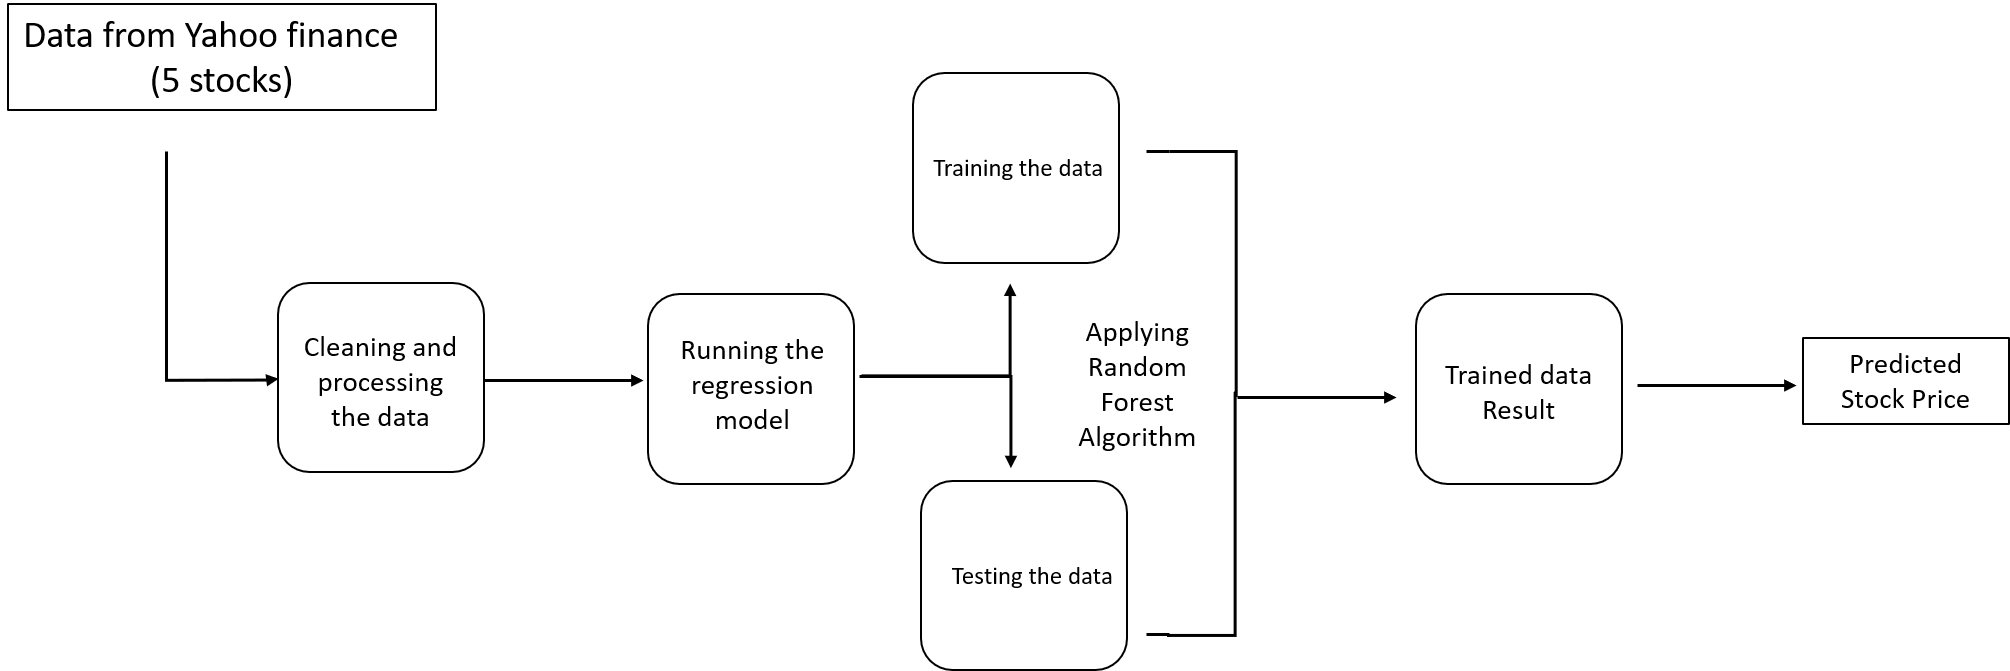
\includegraphics{D:/2017-2018/data_analysis/technical_analysis/report/rflow.png}
\caption{Flow chart of the process}
\end{figure}

\hypertarget{summarizing-the-data}{%
\subsubsection{Summarizing the Data}\label{summarizing-the-data}}

To begin with, we import the data of all the 5 stock prices from Yahoo
finance. In order to have a summary of the data we use different
functions such as \texttt{summary}, which is a generic function used to
produce result summaries of various model fitting functions. Then we use
the \texttt{str} function, which is a solid way to display the structure
of an R object. \texttt{str} will give the output of the information on
one line for each basic structure. The \texttt{dim} function gives the
number of dimensions in the data.

This file shows all the prices of Air Liquide with all the 19 variables
for six years, from 2013-2018.

\begin{Shaded}
\begin{Highlighting}[]
\CommentTok{##Air Liquide}

\NormalTok{AI_FINALDATA}

\KeywordTok{dim}\NormalTok{(AI_FINALDATA)    }\CommentTok{#dimension of the matrix}
\KeywordTok{summary}\NormalTok{(AI_FINALDATA)  }\CommentTok{#summary of the data}
\KeywordTok{str}\NormalTok{(AI_FINALDATA)  }\CommentTok{#structure of the data}
\end{Highlighting}
\end{Shaded}

Therefore, the above code just gives an idea about the dataset which we
will be using in our model.

--\textgreater{}

\hypertarget{training-the-machine}{%
\subsubsection{Training the machine}\label{training-the-machine}}

This phase consists of feeding the algorithm with the training data so
that the model can understand the pattern of the data. Here is the code
for dividing the data into train and test data. Before dividing, we need
some packages which are required to get the result we want.

\begin{Shaded}
\begin{Highlighting}[]
\KeywordTok{library}\NormalTok{(party)}
\CommentTok{#install caret package}
\KeywordTok{install.packages}\NormalTok{(}\StringTok{'caret'}\NormalTok{)}
\CommentTok{#load package}
\KeywordTok{set.seed}\NormalTok{(}\DecValTok{123}\NormalTok{)}
\KeywordTok{library}\NormalTok{(caret)}
\NormalTok{trainAI =}\StringTok{ }\KeywordTok{createDataPartition}\NormalTok{(AI_FINALDATA}\OperatorTok{$}\NormalTok{AI.PA.Close,}
                                 \DataTypeTok{p=}\FloatTok{0.7}\NormalTok{, }\DataTypeTok{list=}\OtherTok{FALSE}\NormalTok{,}\DataTypeTok{times=}\DecValTok{1}\NormalTok{)}

\NormalTok{train_}\DecValTok{1}\NormalTok{ =}\StringTok{ }\NormalTok{AI_FINALDATA[}\DecValTok{1}\OperatorTok{:}\DecValTok{1075}\NormalTok{,]    }\CommentTok{#1075 obs out of 1533}
\NormalTok{test_}\DecValTok{1}\NormalTok{ =}\StringTok{ }\NormalTok{AI_FINALDATA[}\DecValTok{1076}\OperatorTok{:}\DecValTok{1533}\NormalTok{,]    }\CommentTok{#458 obss out of 1533}
\end{Highlighting}
\end{Shaded}

\texttt{party} (library) - used for recursive partitioning

\texttt{caret} - (Classification And Regression Training) is a set of
functions that attempt to streamline the process for creating predictive
models. This package is very important for dividing the data into two.

\texttt{set.seed} - Set the seed of R's random number generator, which
is useful for creating simulations or random objects that can be
reproduced.

\texttt{createDataPartition} - A series of test/training partitions are
created using createDataPartition while createResample creates one or
more bootstrap samples. The main function which is used to split the
data.

Now we will use these two datasets for predicting the stock prices and
applying the random forest algorithm.

\hypertarget{data-scoring}{%
\subsubsection{Data Scoring}\label{data-scoring}}

The method of applying a predictive model to a dataset is called the
scoring data process according to \citet{HibaSadia2019}. The last part
of this module describes how the result of the model can infer whether a
stock will rise or sink, based on certain parameters. It also shows the
vulnerabilities of a particular stock or entity.

\begin{Shaded}
\begin{Highlighting}[]
\CommentTok{#random forest parameters}
\CommentTok{#fitting the model or creating the forest}
\KeywordTok{library}\NormalTok{(randomForest)}
\NormalTok{output.forestAI <-}\StringTok{ }\KeywordTok{randomForest}\NormalTok{(AI.PA.Close }\OperatorTok{~}\StringTok{  }\NormalTok{Interest.rates }\OperatorTok{+}\StringTok{ }
\NormalTok{ExchangeRate }\OperatorTok{+}\StringTok{ }\NormalTok{PoliticalStability }\OperatorTok{+}\StringTok{ }\NormalTok{Infaltion }\OperatorTok{+}\StringTok{ }\NormalTok{AirLiquideDividend }
\OperatorTok{+}\StringTok{ }\NormalTok{REVENUE }\OperatorTok{+}\StringTok{ }\NormalTok{NET.INCOME }\OperatorTok{+}\StringTok{ }\NormalTok{Basic.earnings.per.share }\OperatorTok{+}\StringTok{ }\NormalTok{Diluted.earnings.per.share }
\OperatorTok{+}\StringTok{ }\NormalTok{TOTAL.ASSETS  }\OperatorTok{+}\StringTok{ }\NormalTok{INTANGIBLE.ASSETS }\OperatorTok{+}\StringTok{ }\NormalTok{PPE }\OperatorTok{+}\StringTok{ }\NormalTok{CASH  }\OperatorTok{+}\StringTok{  }\NormalTok{TOTAL.EQUITY }
\OperatorTok{+}\StringTok{ }\NormalTok{NON.CURRENT.LIABILITY }\OperatorTok{+}\StringTok{ }\NormalTok{Cash.flows.from.operating.activities }\OperatorTok{+}\StringTok{ }
\NormalTok{Net.cash.flows.from.investing.activities }\OperatorTok{+}\StringTok{ }
\NormalTok{Net.cash.flows.from.financing.activities }\OperatorTok{+}\StringTok{ }
\NormalTok{Net.cash.and.cash.equivalents, train_}\DecValTok{1}\NormalTok{)}

\CommentTok{# View the forest results.}
\KeywordTok{print}\NormalTok{(output.forestAI) }
\end{Highlighting}
\end{Shaded}

\texttt{mtry} = number of variables selected at each split. lower
\texttt{mtry} means less correlation between trees

\texttt{randomForest}(library) - implements Breiman's random forest
algorithm (based on Breiman and Cutler's original Fortran code) for
classification and regression. It can also be used in unsupervised mode
for assessing proximities among data points.

the output gives an object of class randomForest, which is a list with
the following components:

\texttt{call}:the original call to randomForest

\texttt{type}: regression

\texttt{predicted}: the predicted values of the input data based on
out-of-bag samples.

Type of random forest: regression Number of trees: 500 No.~of variables
tried at each split: 6

From the plot we can observe that in the case of Air Liquide, Interest
rate has a significant impact on closing price.

\begin{Shaded}
\begin{Highlighting}[]
\NormalTok{VI_F=}\KeywordTok{importance}\NormalTok{(output.forestAI)}

\NormalTok{VI_F}

\KeywordTok{write.csv}\NormalTok{(VI_F , }\StringTok{"VI_FAI.csv"}\NormalTok{)}


\KeywordTok{varImpPlot}\NormalTok{(output.forestAI,}\DataTypeTok{type=}\DecValTok{2}\NormalTok{)}
\end{Highlighting}
\end{Shaded}

\begin{figure}
\centering
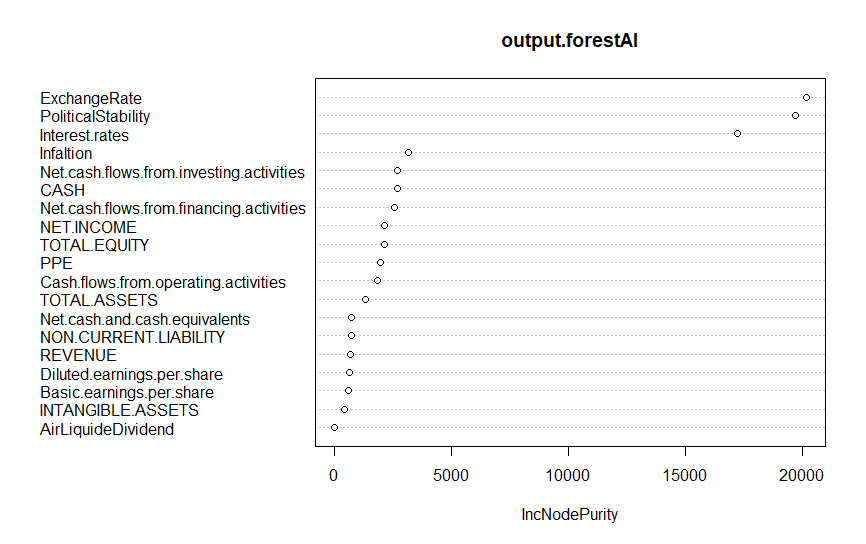
\includegraphics{D:/2017-2018/data_analysis/technical_analysis/report/AI.Plot.png}
\caption{Random Forest of Air Liquide}
\end{figure}

\texttt{IncNodePurity} relates to the loss function that determines how
splits are chosen.

\texttt{importance} - A matrix that measures the importance of each
predictor variable. Columns show different measures of importance.
\texttt{varImplot} - the importance of the variables that were plotted.

The result we get by VI\_F is that again Interest rate is the factor by
which we get the best splits to understand our data.

\hypertarget{experimental-results}{%
\subsubsection{Experimental Results}\label{experimental-results}}

Now, with the help of our random forest and datasets , we will predict
the future prices and we will check how accurate are the results. This
will be done by getting a confusion matrix. A confusion matrix
calculates a cross-tabulation of observed and predicted classes with
associated statistics. In short, it compares the actual values and the
predicted values so that we can get to know how reliable are our
predictions.

\begin{Shaded}
\begin{Highlighting}[]
\CommentTok{#Predictions}

\NormalTok{PredictionsAdjusted <-}\StringTok{ }\KeywordTok{predict}\NormalTok{(output.forestAI, test_}\DecValTok{1}\NormalTok{, }\DataTypeTok{type=}\StringTok{'response'}\NormalTok{)}
\NormalTok{t <-}\StringTok{ }\KeywordTok{table}\NormalTok{(}\DataTypeTok{predictions=}\NormalTok{PredictionsAdjusted, }\DataTypeTok{actual=}\NormalTok{test_}\DecValTok{1}\OperatorTok{$}\NormalTok{AI.PA.Close)}
\NormalTok{t}
\KeywordTok{write.csv}\NormalTok{(t , }\StringTok{"ConfusionMatrix_AI.csv"}\NormalTok{)}
\end{Highlighting}
\end{Shaded}

This gives the Confusion Matrix for Air Liquide.

\begin{Shaded}
\begin{Highlighting}[]
\CommentTok{#Accuracy Metric}
\KeywordTok{sum}\NormalTok{(}\KeywordTok{diag}\NormalTok{(t))}\OperatorTok{/}\KeywordTok{sum}\NormalTok{(t)}
\end{Highlighting}
\end{Shaded}

The accuracy metric in random forest gives the percentage of how
accurate the predictions are. In our case, the accuracy metric is given
below:

\begin{Shaded}
\begin{Highlighting}[]
\NormalTok{Accuracy Metric}\OperatorTok{:}\StringTok{ }\FloatTok{0.01310044} \CommentTok{# or 1.31%}
\end{Highlighting}
\end{Shaded}

This has a very low value which means that we are only 1\% accurate in
predicting our prices. The reason behind this low accuracy rate is that
we have only considered a few variables, as in the real life scenario
there are many variables including the opening, high and low prices of
the same day, which are ignored in this case. Furthermore, there are
other variables which cannot be quantified leading to lack of accuracy.
However, another reason is that with an increase in the number of trees
and \texttt{mtry} (number of splits) we increase the overfitting and
complexity of the model which leads to low accuracy.

\begin{Shaded}
\begin{Highlighting}[]
\CommentTok{#high strength of tree =Low error rate of individual tree classifier}

\NormalTok{PredictionWithProbs <-}\StringTok{ }\KeywordTok{predict}\NormalTok{(output.forestAI, test_}\DecValTok{1}\NormalTok{, }\DataTypeTok{type =} \StringTok{"response"}\NormalTok{)}
\NormalTok{PredictionWithProbs         }\CommentTok{#predicting stock prices for 458 days}
\KeywordTok{write.csv}\NormalTok{(t , }\StringTok{"PredictionsPrices_AI.csv"}\NormalTok{)}
\end{Highlighting}
\end{Shaded}

This function gives 458 predicted values on the basis of the train data
of 1075 observations. This data can be used to develop a trading
strategy where we decide where to invest based on the predictions.

\begin{Shaded}
\begin{Highlighting}[]
\CommentTok{# to find the best "mtry": m try means number of splits at each point. }
\NormalTok{bestmtryAI <-}\StringTok{ }\KeywordTok{tuneRF}\NormalTok{(train_}\DecValTok{1}\NormalTok{,train_}\DecValTok{1}\OperatorTok{$}\NormalTok{AI.PA.Close, }\DataTypeTok{ntreeTry =} \DecValTok{200}\NormalTok{,}
\DataTypeTok{stepFactor =} \FloatTok{1.5}\NormalTok{, }\DataTypeTok{improve =} \FloatTok{0.01}\NormalTok{, }\DataTypeTok{trace =}\NormalTok{ T, }\DataTypeTok{plot=}\NormalTok{ T)}
\end{Highlighting}
\end{Shaded}

\texttt{OOB\ Error} : Out-of-bag error, also called out-of-bag estimate,
is a method to measure the prediction error of random forests, boosted
decision trees.

\begin{figure}
\centering
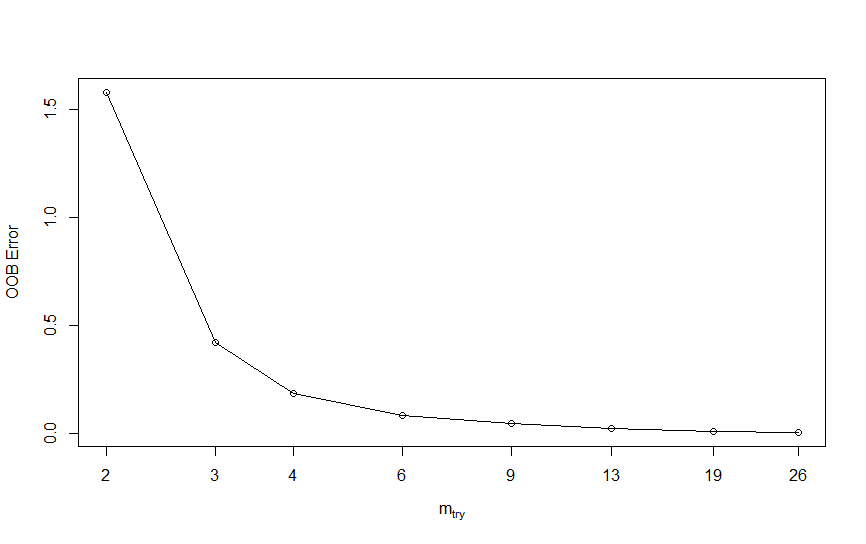
\includegraphics{D:/2017-2018/data_analysis/technical_analysis/report/AI.OBB.png}
\caption{OOB Error of Air Liquide}
\end{figure}

We saw the whole alogrithm applied on the dataset of Air Liquide with 5
years data. Now, we will repeat all the steps above for all other 4
stocks and we will interpret the results for all of them. The output
given below shows the results for the other stocks by using the same
code applied for Air Liquide.

\begin{figure}
\centering
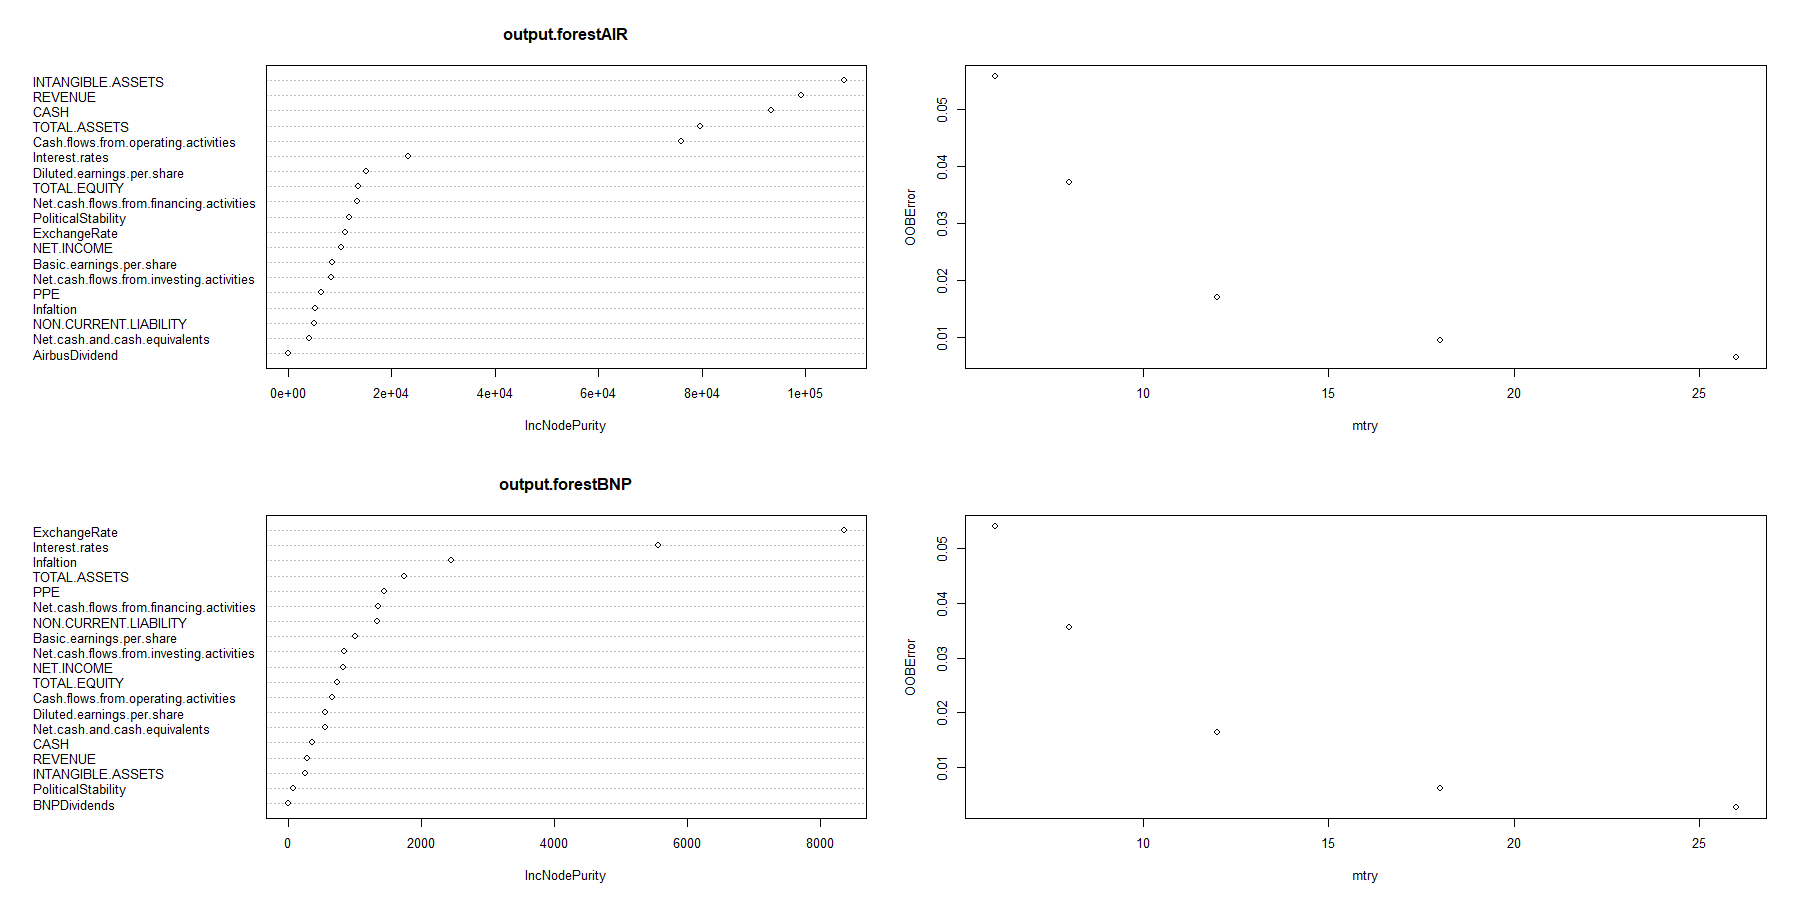
\includegraphics{D:/2017-2018/data_analysis/technical_analysis/report/AIR_BNP.Plot.png}
\caption{RANDOM FOREST AND OOB ERRORS FOR AIRBUS AND BNP PARIBAS}
\end{figure}

\begin{figure}
\centering
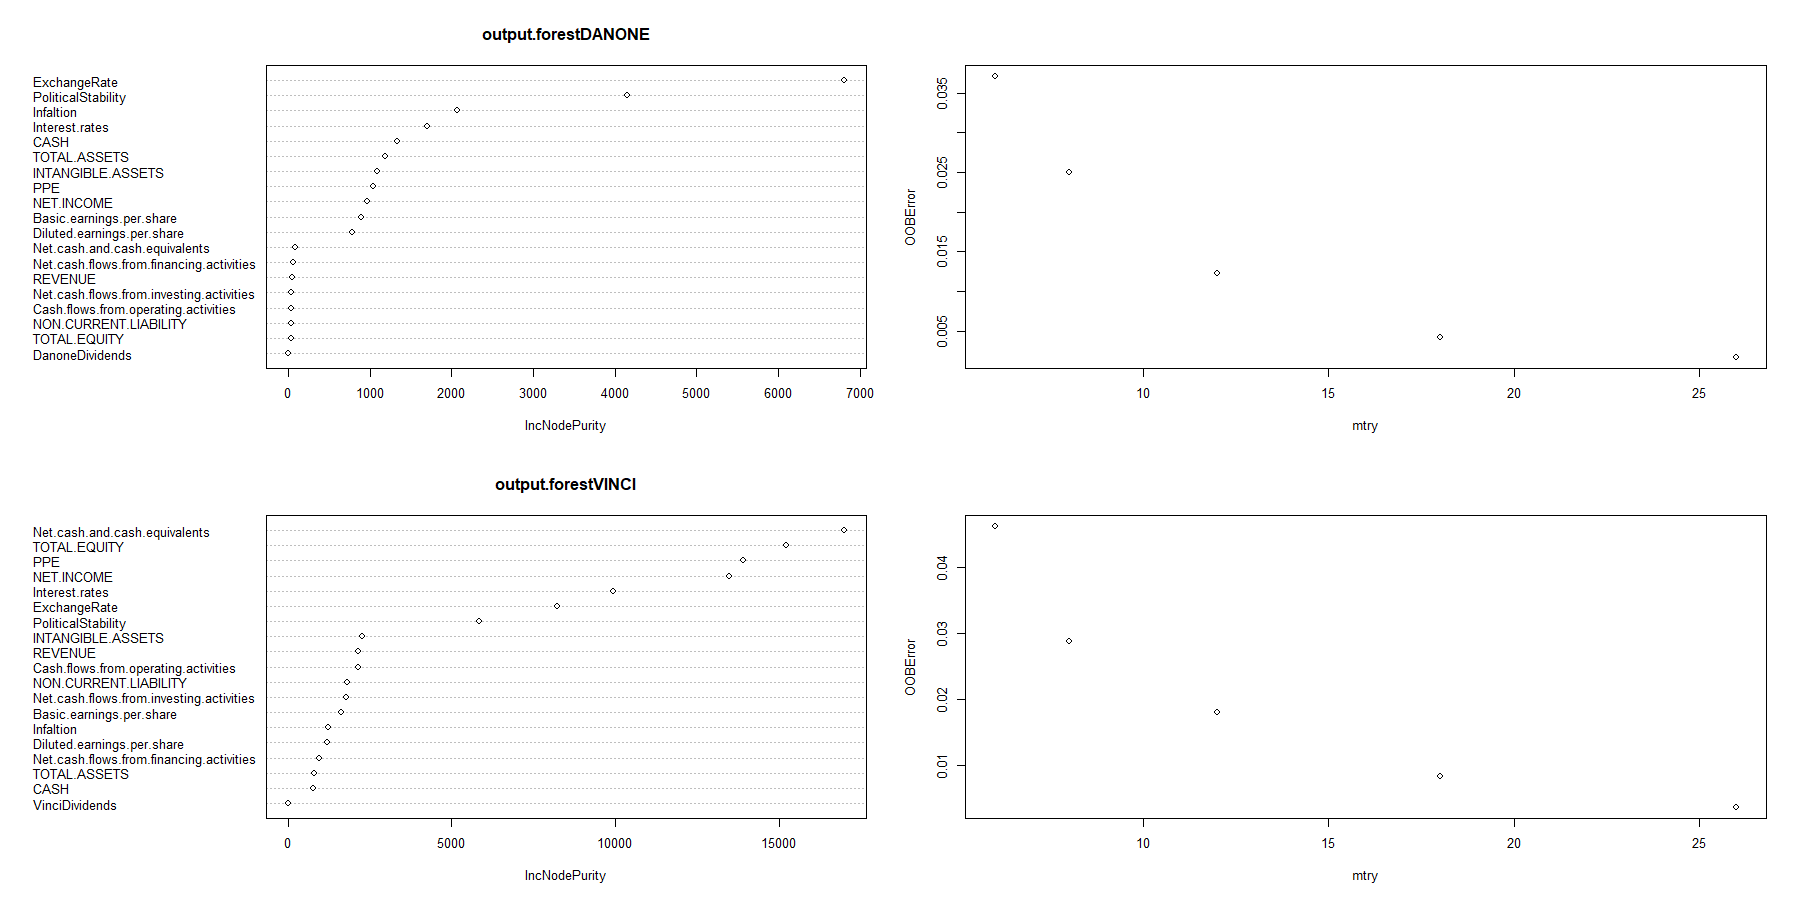
\includegraphics{D:/2017-2018/data_analysis/technical_analysis/report/DANONE_VINCI.Plot.png}
\caption{RANDOM FOREST AND OOB ERRORS FOR DANONE AND VINCI}
\end{figure}

\hypertarget{investment-strategy}{%
\subsection{Investment strategy}\label{investment-strategy}}

In general, the accuracy level of our model is very low for all the five
stocks. Nonetheless, to have a clearer view on its performance, we will
develop an investment strategy based on it and analyze the results. The
graph below compares the predictions of the 5 stocks from 15/03/2017 to
31/12/2018.

\begin{figure}
\centering
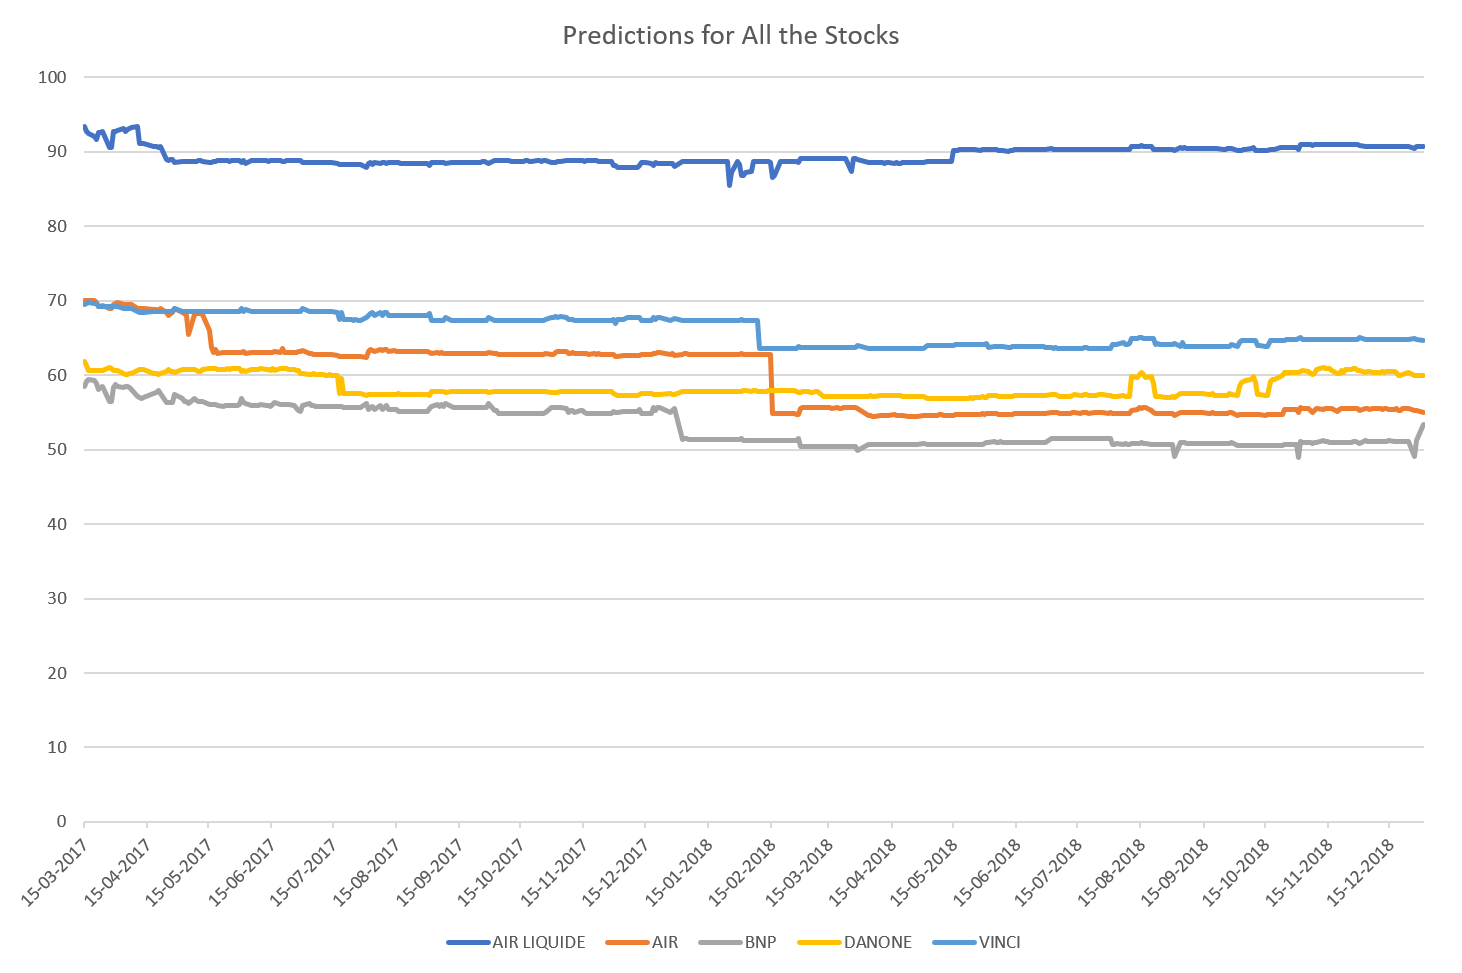
\includegraphics{D:/2017-2018/data_analysis/technical_analysis/report/Predictions.Combined.png}
\caption{Predictions of All the 5 Stocks}
\end{figure}

The investing strategy executed is the same one used in Part 4 for the
neuronal network models. We buy today the stock that, according to our
model, will have the higher increase in price tomorrow, and sell the
stock the day after, repeating the process every day.

The benchmark strategy consists of a diversified buy and hold
investment:

\begin{longtable}[]{@{}llllllll@{}}
\caption{Diversified Strategies}\tabularnewline
\toprule
\begin{minipage}[b]{0.10\columnwidth}\raggedright
X\strut
\end{minipage} & \begin{minipage}[b]{0.06\columnwidth}\raggedright
AI.PA\strut
\end{minipage} & \begin{minipage}[b]{0.07\columnwidth}\raggedright
AIR.PA\strut
\end{minipage} & \begin{minipage}[b]{0.07\columnwidth}\raggedright
BNP.PA\strut
\end{minipage} & \begin{minipage}[b]{0.06\columnwidth}\raggedright
BN.PA\strut
\end{minipage} & \begin{minipage}[b]{0.06\columnwidth}\raggedright
DG.PA\strut
\end{minipage} & \begin{minipage}[b]{0.19\columnwidth}\raggedright
X.1\strut
\end{minipage} & \begin{minipage}[b]{0.16\columnwidth}\raggedright
Capital\strut
\end{minipage}\tabularnewline
\midrule
\endfirsthead
\toprule
\begin{minipage}[b]{0.10\columnwidth}\raggedright
X\strut
\end{minipage} & \begin{minipage}[b]{0.06\columnwidth}\raggedright
AI.PA\strut
\end{minipage} & \begin{minipage}[b]{0.07\columnwidth}\raggedright
AIR.PA\strut
\end{minipage} & \begin{minipage}[b]{0.07\columnwidth}\raggedright
BNP.PA\strut
\end{minipage} & \begin{minipage}[b]{0.06\columnwidth}\raggedright
BN.PA\strut
\end{minipage} & \begin{minipage}[b]{0.06\columnwidth}\raggedright
DG.PA\strut
\end{minipage} & \begin{minipage}[b]{0.19\columnwidth}\raggedright
X.1\strut
\end{minipage} & \begin{minipage}[b]{0.16\columnwidth}\raggedright
Capital\strut
\end{minipage}\tabularnewline
\midrule
\endhead
\begin{minipage}[t]{0.10\columnwidth}\raggedright
15-03-2017\strut
\end{minipage} & \begin{minipage}[t]{0.06\columnwidth}\raggedright
94.55\strut
\end{minipage} & \begin{minipage}[t]{0.07\columnwidth}\raggedright
70.43\strut
\end{minipage} & \begin{minipage}[t]{0.07\columnwidth}\raggedright
60.09\strut
\end{minipage} & \begin{minipage}[t]{0.06\columnwidth}\raggedright
62.62\strut
\end{minipage} & \begin{minipage}[t]{0.06\columnwidth}\raggedright
69.45\strut
\end{minipage} & \begin{minipage}[t]{0.19\columnwidth}\raggedright
stock price(euro)\strut
\end{minipage} & \begin{minipage}[t]{0.16\columnwidth}\raggedright
Total budget(euro)\strut
\end{minipage}\tabularnewline
\begin{minipage}[t]{0.10\columnwidth}\raggedright
\strut
\end{minipage} & \begin{minipage}[t]{0.06\columnwidth}\raggedright
2000\strut
\end{minipage} & \begin{minipage}[t]{0.07\columnwidth}\raggedright
2000\strut
\end{minipage} & \begin{minipage}[t]{0.07\columnwidth}\raggedright
2000\strut
\end{minipage} & \begin{minipage}[t]{0.06\columnwidth}\raggedright
2000\strut
\end{minipage} & \begin{minipage}[t]{0.06\columnwidth}\raggedright
2000\strut
\end{minipage} & \begin{minipage}[t]{0.19\columnwidth}\raggedright
amount invested(euro)\strut
\end{minipage} & \begin{minipage}[t]{0.16\columnwidth}\raggedright
10000\strut
\end{minipage}\tabularnewline
\begin{minipage}[t]{0.10\columnwidth}\raggedright
\strut
\end{minipage} & \begin{minipage}[t]{0.06\columnwidth}\raggedright
21.15\strut
\end{minipage} & \begin{minipage}[t]{0.07\columnwidth}\raggedright
28.4\strut
\end{minipage} & \begin{minipage}[t]{0.07\columnwidth}\raggedright
33.28\strut
\end{minipage} & \begin{minipage}[t]{0.06\columnwidth}\raggedright
31.94\strut
\end{minipage} & \begin{minipage}[t]{0.06\columnwidth}\raggedright
28.8\strut
\end{minipage} & \begin{minipage}[t]{0.19\columnwidth}\raggedright
N. of shares bought\strut
\end{minipage} & \begin{minipage}[t]{0.16\columnwidth}\raggedright
\strut
\end{minipage}\tabularnewline
\begin{minipage}[t]{0.10\columnwidth}\raggedright
\strut
\end{minipage} & \begin{minipage}[t]{0.06\columnwidth}\raggedright
NA\strut
\end{minipage} & \begin{minipage}[t]{0.07\columnwidth}\raggedright
NA\strut
\end{minipage} & \begin{minipage}[t]{0.07\columnwidth}\raggedright
NA\strut
\end{minipage} & \begin{minipage}[t]{0.06\columnwidth}\raggedright
NA\strut
\end{minipage} & \begin{minipage}[t]{0.06\columnwidth}\raggedright
NA\strut
\end{minipage} & \begin{minipage}[t]{0.19\columnwidth}\raggedright
\strut
\end{minipage} & \begin{minipage}[t]{0.16\columnwidth}\raggedright
\strut
\end{minipage}\tabularnewline
\begin{minipage}[t]{0.10\columnwidth}\raggedright
31-12-2018\strut
\end{minipage} & \begin{minipage}[t]{0.06\columnwidth}\raggedright
98.59\strut
\end{minipage} & \begin{minipage}[t]{0.07\columnwidth}\raggedright
83.96\strut
\end{minipage} & \begin{minipage}[t]{0.07\columnwidth}\raggedright
39.47\strut
\end{minipage} & \begin{minipage}[t]{0.06\columnwidth}\raggedright
61.51\strut
\end{minipage} & \begin{minipage}[t]{0.06\columnwidth}\raggedright
72.02\strut
\end{minipage} & \begin{minipage}[t]{0.19\columnwidth}\raggedright
stock price(euro)\strut
\end{minipage} & \begin{minipage}[t]{0.16\columnwidth}\raggedright
Total budget(euro)\strut
\end{minipage}\tabularnewline
\begin{minipage}[t]{0.10\columnwidth}\raggedright
\strut
\end{minipage} & \begin{minipage}[t]{0.06\columnwidth}\raggedright
2086\strut
\end{minipage} & \begin{minipage}[t]{0.07\columnwidth}\raggedright
2384\strut
\end{minipage} & \begin{minipage}[t]{0.07\columnwidth}\raggedright
1314\strut
\end{minipage} & \begin{minipage}[t]{0.06\columnwidth}\raggedright
1965\strut
\end{minipage} & \begin{minipage}[t]{0.06\columnwidth}\raggedright
2074\strut
\end{minipage} & \begin{minipage}[t]{0.19\columnwidth}\raggedright
value in stocks(euro)\strut
\end{minipage} & \begin{minipage}[t]{0.16\columnwidth}\raggedright
9822.21\strut
\end{minipage}\tabularnewline
\bottomrule
\end{longtable}

The table above shows the diversified strategy according to which, we
would get a negative return on our investment of -0.018. This implies
that the diversified strategy would result in a loss for the investor.

The file PA contains all the predictions we found out from 15/03/2017 to
31/12/2018 for all the 5 stocks. The file DAT contains all the real
closing prices of all the 5 stocks from 14/03/2017 to 28/12/2018. In the
code below, we first calculate the predicted day-by-day returns for the
5 stocks and then simulate an investing strategy where we buy everyday
the stock with the highest predicted return, and sell it the day after.

\begin{Shaded}
\begin{Highlighting}[]
\NormalTok{PA}
\NormalTok{DAT}

\NormalTok{RETU <-}\StringTok{ }\NormalTok{(PA}\OperatorTok{-}\NormalTok{DAT)}\OperatorTok{/}\NormalTok{DAT}
\KeywordTok{View}\NormalTok{(RETU)}
\NormalTok{I <-}\StringTok{ }\KeywordTok{c}\NormalTok{()}
\ControlFlowTok{for}\NormalTok{ (n }\ControlFlowTok{in} \DecValTok{1}\OperatorTok{:}\DecValTok{458}\NormalTok{)\{}
    \ControlFlowTok{if}\NormalTok{ (}\KeywordTok{max}\NormalTok{(RETU[n,]) }\OperatorTok{==}\StringTok{ }\NormalTok{RETU[n,}\DecValTok{1}\NormalTok{])\{}
\NormalTok{        I[n] =}\StringTok{ }\DecValTok{1}
\NormalTok{    \} }\ControlFlowTok{else} \ControlFlowTok{if}\NormalTok{ (}\KeywordTok{max}\NormalTok{(RETU[n,]) }\OperatorTok{==}\StringTok{ }\NormalTok{RETU[n,}\DecValTok{2}\NormalTok{])\{}
\NormalTok{        I[n] =}\StringTok{ }\DecValTok{2}
\NormalTok{    \} }\ControlFlowTok{else} \ControlFlowTok{if}\NormalTok{ (}\KeywordTok{max}\NormalTok{(RETU[n,]) }\OperatorTok{==}\StringTok{ }\NormalTok{RETU[n,}\DecValTok{3}\NormalTok{])\{}
\NormalTok{        I[n] =}\StringTok{ }\DecValTok{3}
\NormalTok{    \} }\ControlFlowTok{else} \ControlFlowTok{if}\NormalTok{ (}\KeywordTok{max}\NormalTok{(RETU[n,]) }\OperatorTok{==}\StringTok{ }\NormalTok{RETU[n,}\DecValTok{4}\NormalTok{])\{}
\NormalTok{        I[n] =}\StringTok{ }\DecValTok{4}
\NormalTok{    \} }\ControlFlowTok{else} \ControlFlowTok{if}\NormalTok{ (}\KeywordTok{max}\NormalTok{(RETU[n,]) }\OperatorTok{==}\StringTok{ }\NormalTok{RETU[n,}\DecValTok{5}\NormalTok{])\{}
\NormalTok{        I[n] =}\StringTok{ }\DecValTok{5}
\NormalTok{    \}}
\NormalTok{\}}
\NormalTok{X =}\StringTok{ }\DecValTok{10000}
\ControlFlowTok{for}\NormalTok{ (n }\ControlFlowTok{in} \DecValTok{1}\OperatorTok{:}\DecValTok{456}\NormalTok{)\{}
    \ControlFlowTok{if}\NormalTok{ (I[n] }\OperatorTok{==}\StringTok{ }\DecValTok{1}\NormalTok{)\{}
\NormalTok{        Y =}\StringTok{ }\DecValTok{1}
\NormalTok{    \} }\ControlFlowTok{else} \ControlFlowTok{if}\NormalTok{ (I[n] }\OperatorTok{==}\StringTok{ }\DecValTok{2}\NormalTok{)\{}
\NormalTok{        Y =}\StringTok{ }\DecValTok{2}
\NormalTok{    \} }\ControlFlowTok{else} \ControlFlowTok{if}\NormalTok{ (I[n] }\OperatorTok{==}\StringTok{ }\DecValTok{3}\NormalTok{)\{}
\NormalTok{        Y =}\StringTok{ }\DecValTok{3}
\NormalTok{    \} }\ControlFlowTok{else} \ControlFlowTok{if}\NormalTok{ (I[n] }\OperatorTok{==}\StringTok{ }\DecValTok{4}\NormalTok{)\{}
\NormalTok{        Y =}\StringTok{ }\DecValTok{4}
\NormalTok{    \} }\ControlFlowTok{else} \ControlFlowTok{if}\NormalTok{ (I[n] }\OperatorTok{==}\StringTok{ }\DecValTok{5}\NormalTok{)\{}
\NormalTok{        Y =}\StringTok{ }\DecValTok{5}
\NormalTok{    \}}
\NormalTok{    X =}\StringTok{ }\NormalTok{X}\OperatorTok{*}\NormalTok{(DAT[n}\OperatorTok{+}\DecValTok{2}\NormalTok{,Y]}\OperatorTok{/}\NormalTok{DAT[n}\OperatorTok{+}\DecValTok{1}\NormalTok{,Y])}
\NormalTok{\}}
\KeywordTok{View}\NormalTok{(X)   }
\end{Highlighting}
\end{Shaded}

We see that, following the random forest algorithm, starting with 10,000
euro, we would end up with 10014.39 euro after 1 year and 8 months of
trading. This shows that the strategy outperforms the passive investment
but a return of 0.14\% after 20 months is far from being an ideal
scenario.

\hypertarget{comments-and-future-implementation}{%
\subsection{Comments and Future
Implementation}\label{comments-and-future-implementation}}

Future steps for this analysis would be to get rid of drawbacks of the
model and try to attain a higher level of accuracy by using more complex
random forest functions and adding other parameters which could impact
price. The additional use of traditional algorithms and data mining
techniques could also improve the predictability power of the model.

\newpage

\renewcommand\refname{References}
  \bibliography{bibliography.bib}

\end{document}
